% Pass options to the xcolor package for table support
\PassOptionsToPackage{table}{xcolor}

% Document class: A4 paper with an 6pt font size.
\documentclass[a4paper,6pt]{article}

% Use a plain page style (no headers/footers beyond page numbers)
\pagestyle{plain}

% Import the base preamble (packages, macros, environments, etc.)
% -----------------------------
% Document Class & Encoding
% -----------------------------
\usepackage[utf8]{inputenc}  % Input encoding
\usepackage[T1]{fontenc}     % Font encoding

% -----------------------------
% Page Layout & Geometry
% -----------------------------
\usepackage[margin=2cm,foot=1cm]{geometry}

% -----------------------------
% Header & Footer Management
% -----------------------------
\usepackage{fancyhdr}
\pagestyle{fancy}

% -----------------------------
% Text Formatting & Spacing
% -----------------------------
\usepackage{ragged2e}
\usepackage[nodisplayskipstretch]{setspace}
\setstretch{1}  % Line spacing

% -----------------------------
% Hyperlinks
% -----------------------------
\usepackage{hyperref}
\hypersetup{
  colorlinks,
  linkcolor={blue!80!black},
  citecolor={green!80!black},
  urlcolor={red!80!black}
}

% -----------------------------
% Bibliography Support
% -----------------------------
\usepackage{natbib}

% -----------------------------
% Listings for Code
% -----------------------------
\usepackage{listings}
\usepackage{xcolor}

% -----------------------------
% Tables, Figures & Graphics
% -----------------------------
\usepackage{tabularx}
\usepackage{pdflscape}
\usepackage{graphicx}

% -----------------------------
% Algorithms
% -----------------------------
\usepackage{algorithm}       % For floating algorithm environment
\usepackage{algpseudocode}   % For pseudo-code inside algorithms

% -----------------------------
% Math Packages
% -----------------------------
\usepackage{amsmath,amssymb,amsthm,mathtools,bm}
\usepackage{mathrsfs}        % Script fonts
\usepackage{tikz-cd}         % Commutative diagrams
\usepackage{rotating}        % Rotated objects
\usepackage{float}           % Float placement
\usetikzlibrary{calc, arrows, positioning, arrows.meta}

% -----------------------------
% TikZ and its Libraries
% -----------------------------
\usepackage{tikz}
\usetikzlibrary{positioning} % Added to support "below=of" syntax

% -----------------------------
% Miscellaneous Packages
% -----------------------------
\usepackage{xparse}          % For defining robust commands
\usepackage{enumitem}        % For customizing list layouts
\usepackage{makecell}        % For enhanced table cells
\usepackage{comment}		 % For commenting out sections

%%%%%%%%%%%%%%%%%%%%%%%%%%%%%%%%%%%%%%%%%%%%%%%%%%%%%%%%%%%%%%%%%%%%%%%%%%%%%%%
% Custom Math Commands and Shortcuts
%%%%%%%%%%%%%%%%%%%%%%%%%%%%%%%%%%%%%%%%%%%%%%%%%%%%%%%%%%%%%%%%%%%%%%%%%%%%%%%

% Matrix and Vector Formatting
\newcommand{\matr}[1]{\mathbf{#1}}      % For undergraduate algebra (alternative: \bm{#1})
\newcommand{\vect}[1]{\bm{#1}}

% Standard Number Sets
\newcommand{\N}{\mathbb{N}}
\newcommand{\R}{\mathbb{R}}
\newcommand{\Q}{\mathbb{Q}}
\newcommand{\C}{\mathbb{C}}
\newcommand{\Z}{\mathbb{Z}}

% Bold variables (customize as needed)
\newcommand{\x}{\mathbf{x}}
\newcommand{\F}{\mathbf{F}}
\newcommand{\f}{\mathbf{f}}
\newcommand{\y}{\mathbf{y}}
\renewcommand{\a}{\mathbf{a}}
\renewcommand{\b}{\mathbf{b}}
\renewcommand{\c}{\mathbf{c}}
\newcommand{\h}{\mathbf{h}}
\newcommand{\g}{\mathbf{g}}
\newcommand{\z}{\mathbf{z}}
\newcommand{\ze}{\mathbf{0}}

% Norms, Absolute Values, and Bracketing
\newcommand{\norm}[1]{\left\lVert#1\right\rVert}
\newcommand{\abs}[1]{\left\lvert#1\right\rvert}
\newcommand{\brk}[1]{\left[#1\right]}
\newcommand{\brc}[1]{\left\{#1\right\}}
\newcommand{\paren}[1]{\left(#1\right)}
\newcommand{\normop}[1]{\left\lVert#1\right\rVert_\text{op}}

% Miscellaneous Math Shortcuts
\newcommand{\LL}{\mathcal{L}}
\newcommand{\uni}{\overset{\text{uni}}{\to}}
\DeclareMathOperator{\diam}{diam}
\newcommand{\Prr}[1]{\text{Pr}\left(#1\right)}
\newcommand{\ceil}[1]{\lceil #1 \rceil}
\newcommand{\floor}[1]{\lfloor #1 \rfloor}
\newcommand\disteq{\stackrel{\textnormal{dist}}{=}}

% Evaluation command with options
\NewDocumentCommand{\evalat}{sO{\big}mm}{%
  \IfBooleanTF{#1}
    {\mleft. #3 \mright|_{#4}}
    {#3#2|_{#4}}%
}

%%%%%%%%%%%%%%%%%%%%%%%%%%%%%%%%%%%%%%%%%%%%%%%%%%%%%%%%%%%%%%%%%%%%%%%%%%%%%%%
% Color Definitions
%%%%%%%%%%%%%%%%%%%%%%%%%%%%%%%%%%%%%%%%%%%%%%%%%%%%%%%%%%%%%%%%%%%%%%%%%%%%%%%

\definecolor{dartmouthgreen}{rgb}{0.05, 0.5, 0.06}
\definecolor{egyptianblue}{rgb}{0.06, 0.2, 0.65}
\definecolor{dukeblue}{rgb}{0.0, 0.0, 0.61}
\definecolor{jazzberryjam}{rgb}{0.65, 0.04, 0.37}
\definecolor{magenta}{HTML}{EC008C}
\definecolor{darkmagenta}{rgb}{0.55, 0.0, 0.55}
\definecolor{deeppink}{rgb}{1.0, 0.08, 0.58}
\definecolor{codegreen}{rgb}{0,0.6,0}
\definecolor{codegray}{rgb}{0.5,0.5,0.5}
\definecolor{codepurple}{rgb}{0.58,0,0.82}
\definecolor{backcolour}{rgb}{0.95,0.95,0.92}

%%%%%%%%%%%%%%%%%%%%%%%%%%%%%%%%%%%%%%%%%%%%%%%%%%%%%%%%%%%%%%%%%%%%%%%%%%%%%%%
% Custom Shortcuts and Emphasis Commands
%%%%%%%%%%%%%%%%%%%%%%%%%%%%%%%%%%%%%%%%%%%%%%%%%%%%%%%%%%%%%%%%%%%%%%%%%%%%%%%

\newcommand{\isomorp}{\xrightarrow{\sim}}
\newcommand{\hlt}[1]{\textit{{\color{blue}#1}}}
\newcommand{\simpt}[1]{\textit{{\color{deeppink}#1}}}
\newcommand{\impt}[1]{\textit{{\color{red}#1}}}
\newcommand{\gcds}[1]{\textnormal{gcd}#1}
\newcommand{\mins}[1]{\textnormal{min}#1}
\newcommand{\maxs}[1]{\textnormal{max}#1}
\newcommand{\lcms}[1]{\textnormal{lcm}#1}
\newcommand{\degs}[1]{\textnormal{deg}#1}
\newcommand{\exps}[1]{\textnormal{exp}#1}
\newcommand{\tors}[1]{\textnormal{Tor}#1}
\newcommand{\homs}[1]{\textnormal{Hom}#1}
\newcommand{\anns}[1]{\textnormal{Ann}#1}
\DeclareMathOperator{\sign}{sign}

%%%%%%%%%%%%%%%%%%%%%%%%%%%%%%%%%%%%%%%%%%%%%%%%%%%%%%%%%%%%%%%%%%%%%%%%%%%%%%%
% Theorem and Definition Environments
%%%%%%%%%%%%%%%%%%%%%%%%%%%%%%%%%%%%%%%%%%%%%%%%%%%%%%%%%%%%%%%%%%%%%%%%%%%%%%%

\theoremstyle{theorem}
\newtheorem{theorem}{Theorem}[subsection]
\newtheorem{corollary}[theorem]{Corollary}
\newtheorem{lemma}[theorem]{Lemma}
\newtheorem{proposition}[theorem]{Proposition}
\newtheorem{qnbank}[theorem]{Question Bank}
\let\oldqnbank\qnbank
\renewcommand{\qnbank}{\oldqnbank\normalfont}
\newtheorem{process}[theorem]{Process}
\let\oldprocess\process
\renewcommand{\process}{\oldprocess\normalfont}
\newtheorem{method}[theorem]{Method}
\let\oldmethod\method
\renewcommand{\method}{\oldmethod\normalfont}
\newtheorem{definition}[theorem]{Definition}
\let\olddefinition\definition
\renewcommand{\definition}{\olddefinition\normalfont}
\newtheorem{example}[theorem]{Example}
\let\oldexample\example
\renewcommand{\example}{\oldexample\normalfont}
\newtheorem{remark}[theorem]{Remark}
\let\oldremark\remark
\renewcommand{\remark}{\oldremark\normalfont}

%%%%%%%%%%%%%%%%%%%%%%%%%%%%%%%%%%%%%%%%%%%%%%%%%%%%%%%%%%%%%%%%%%%%%%%%%%%%%%%
% Breakable Algorithm Environment (Algorithms spanning multiple pages)
%%%%%%%%%%%%%%%%%%%%%%%%%%%%%%%%%%%%%%%%%%%%%%%%%%%%%%%%%%%%%%%%%%%%%%%%%%%%%%%

\makeatletter
\newenvironment{breakablealgorithm}
 {%
  \begin{center}
    \refstepcounter{algorithm} % Increment algorithm counter
    \hrule height.8pt depth0pt \kern2pt
    \renewcommand{\caption}[2][\relax]{%
      {\raggedright\textbf{Algorithm \thealgorithm:} ##2\par}%
      \ifx\relax##1\relax
        \addcontentsline{loa}{algorithm}{\protect\numberline{\thealgorithm}##2}%
      \else
        \addcontentsline{loa}{algorithm}{\protect\numberline{\thealgorithm}##1}%
      \fi
      \kern2pt\hrule\kern2pt
    }%
 }{%
    \kern2pt\hrule
  \end{center}
 }
\makeatother

%%%%%%%%%%%%%%%%%%%%%%%%%%%%%%%%%%%%%%%%%%%%%%%%%%%%%%%%%%%%%%%%%%%%%%%%%%%%%%%
% Code Listings Style
%%%%%%%%%%%%%%%%%%%%%%%%%%%%%%%%%%%%%%%%%%%%%%%%%%%%%%%%%%%%%%%%%%%%%%%%%%%%%%%

\lstdefinestyle{codestyle}{
  commentstyle=\color{codegreen},
  keywordstyle=\color{magenta},
  numberstyle=\tiny\color{codegray},
  stringstyle=\color{codepurple},
  basicstyle=\ttfamily\normalsize,
  breakatwhitespace=false,
  breaklines=true,
  captionpos=b,
  keepspaces=true,
  numbers=left,
  numbersep=10pt,
  frame=single,
  showspaces=false,
  showstringspaces=false,
  showtabs=false,
  tabsize=2
}
\lstset{style=codestyle}




% Set the title and author metadata
\title{Algorithmic Trading}
\author{Arthur Li}

\begin{document}

% Use Roman page numbering for front matter
\pagenumbering{roman}

% Title Page
\maketitle

% Bibliography style (Chicago)
\bibliographystyle{chicago}

% Table of Contents
\newpage
\tableofcontents

% Switch to Arabic numbering for main content pages
\newpage
\pagenumbering{arabic}

% Introduction Section
\newpage
\section{Preface and Prerequisites}

\subsection{Brief Overview}

Lorem Ipsum\\
To be completed once most of the book is done


\subsection{Reading Roadmap}

Lorem Ipsum. To be completed once most of the book is done\\

This content builds upon the foundational works of Rishi K. \cite{rishi_2013}, Raja \cite{velu_2020}, and Marcos Lopez \cite{marcos_2018}, among others, whose insights form the backbone of our discussion.

\newpage

\subsection{Overview of Systematic Investments}

A schematic of a live 'production' trading strategy is shown below, but does not include everything else necessary to create the strategy (i.e., research tools).

\begin{figure}[H]
\centering
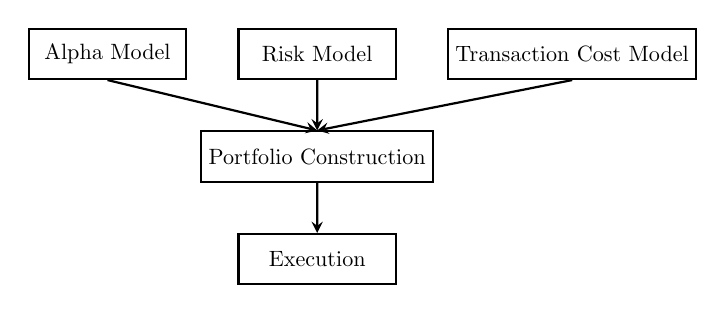
\begin{tikzpicture}[auto, thick, >=stealth, scale=0.8, transform shape]

    \usetikzlibrary{positioning}

    % Three modules arranged horizontally with reduced dimensions
    \node[draw, rectangle, minimum width=2.5cm, minimum height=0.8cm] (alpha) {Alpha Model};
    \node[draw, rectangle, minimum width=2.5cm, minimum height=0.8cm, right=0.8cm of alpha] (risk) {Risk Model};
    \node[draw, rectangle, minimum width=2.5cm, minimum height=0.8cm, right=0.8cm of risk] (tc) {Transaction Cost Model};

    % Portfolio Construction node directly below Risk Model
    \node[draw, rectangle, minimum width=2.5cm, minimum height=0.8cm, below=0.8cm of risk] (portfolio) {Portfolio Construction};

    % Execution node below Portfolio Construction
    \node[draw, rectangle, minimum width=2.5cm, minimum height=0.8cm, below=0.8cm of portfolio] (execution) {Execution};

    % Arrows connecting the nodes
    \draw[->] (alpha.south) -- (portfolio.north);
    \draw[->] (risk.south) -- (portfolio.north);
    \draw[->] (tc.south) -- (portfolio.north);
    \draw[->] (portfolio.south) -- (execution.north);
    
\end{tikzpicture}



\caption{Live Production Trading Strategy Overview}
\end{figure}

At its core, the trading system is organised into three primary modules:

The trading system has three modules:
\begin{enumerate}[label=\roman*.]
\setlength{\itemsep}{0pt}
\item Alpha model: predicts the future of the instruments considered for trading, i.e. directional alpha
\item Risk model: limits amount of exposure to factors that are unlikely to generate returns but could drive losses, i.e. directional exposure limit on an asset class
\item Transaction cost model: determine if the cost of the trades needed to migrate from current portfolio to new portfolio is desirable to the portfolio construction model.
\end{enumerate}
These models feed into a portfolio construction model that balances the tradeoffs of profit and risk to determine the best portfolio to hold. The model finds the differences in trades that need to be executed.\\
The execution model then takes the required trades, and using inputs such as urgency in which the trades need to be executed and dynamics of liquidity in the markets, executes the trades in an efficient and low cost manner.\\

\begin{method} \hlt{Chains of Production for Alpha Signals}
\begin{enumerate}[label=\roman*.]
\setlength{\itemsep}{0pt}
\item Data Curation: for collecting, cleaning, indexing, storing, adjusting, and delivering all data to production chain. Requires experts in market microstructure and data protocols such as FIX.
\item Feature Analysis: transform raw data into informative signals. Requires experts in information theory, signal extraction and processing, visualisation, labelling, weighting, classifiers, feature importance techniques. Feature analysts collect and catalogue libraries of findings.
\item Strategists: informative features are transformed into actual investment algorithms. Strategists will parse libraries of features for ideas to develop an investment strategy. Require data scientists with deep knowledge of financial markets and economy. Features may be discovered by black box, but strategy is developed in a white box.
\item Back-testers: assess profitability of investment strategy under various scenarios. Requires data scientists with deep understanding of empirical and experimental techniques. Good back-tested incorporates in analysis meta-information on how strategy was created.
\item Deployment Team: integrate strategy code into production line. Requires algorithm specialists and mathematical programmers. To ensure deployed solution is logically identical to prototype, and to optimise implementation sufficiently such that production latency is minimised.
\item Portfolio Oversight: once strategy is deployed, follows lifecycle.
\begin{enumerate}[label=\arabic*.]
\setlength{\itemsep}{0pt}
\item Embargo: initially, strategy is run on data observed after end date of backtest. If embargoed performance is consistent with backtest, strategy is promoted to next stage.
\item Paper Trading: strategy run on live, real-time feed. Performance accounts for data parsing latencies, calculation latencies, execution delays, and other time lapses between observation and positioning. 
\item Graduation: strategy manages real position, whether in isolation of as part of ensemble. Performance evaluated precisely, including attributed risk, returns, and costs.
\item Re-allocation: based on production performance, allocation is re-assessed frequently and automatically. Strategy allocation follows a concave function, Initial allocation is small. As time passes and strategy performs as expected, allocation is increased. Over time, performance decays and allocations become gradually smaller.
\item Decommission: if strategy perform below expectations for sufficiently extended period of time, strategy is discontinued.
\end{enumerate}
\end{enumerate}
\end{method}

\subsubsection{Alpha Models Overview}

Theory-driven models tests theories of why markets behave in a manner, and see if they can be used to predict the future. Strategies utilising price-related data are trend and mean reversion; strategies utilising fundamental data are value/yield, growth and quality. Usually more than one model is used in combination.

\begin{definition} \hlt{Theory Driven Models}
\begin{enumerate}[label=\roman*.]
\setlength{\itemsep}{0pt}
\item Trend Following: markets move in given direction long enough that the trend can be identified. As more data support the bull/bear thesis in an uncertain market, more market participants will adopt the same thesis and hence move the asset price to a new equilibrium.\\
Moving average crossover indicator strategy has less than one point of return for every point of downside risk taken, as market behaviour are unstable and episodic.
\item Mean Reversion: markets move in opposite direction to the prevailing trend. Short-term imbalances between buyers and sellers due to liquidity forces prices to move abruptly in one direction, which increases probability of trend reversion as liquidity issue is resolved.\\
Statistical arbitrage bets on convergence of prices of similar stocks whose prices have diverged.\\
Longer-term trends can occur despite smaller oscillations around these trends occurring in the shorter term, hence both strategies may be used in conjunction.
\item Value/Yield:  value strategies uses ratios of fundamental factor against the price of the instrument, inverted to keep the ratio consistent. The higher the yield, the cheaper the instrument.\\
Buying undervalued security and selling overvalued security is a \hlt{carry trade}. The difference between yield received and yield paid is the \hlt{carry}.\\
\hlt{Quant Long Short (QLS)} ranks stocks by attractiveness based on various factors such as value, then buy the higher-ranked stocks while shorting the lower-ranked stocks.
\item Growth: make predictions based on asset's expected or historically observed level of economic growth. Forward-looking growth expectations are typically used as a metric.\\
Growth is trending, and strongest growers are becoming more dominant relative to competitors. Macro growth factors may be used on foreign exchange, while micro growth factors may be used on companies.
\item Quality: All else being equal, it is better to long high quality and short low quality. Capital safety is important. Factors include earnings quality, equity-to-debt ratios etc.
\end{enumerate}
\end{definition}

Data-driven models are more difficult to understand, with more complicated mathematics. Relies on data mining, more technically challenging and far less widely practiced. Typically more used in high-frequency space, as they can discern how market behaves without caring about the economic theory or rational.

\begin{method} \hlt{Strategy Parameters}\\
An implementation approach requires a forecast target, time horizon, bet structure, investment universe, model specification, and run frequency.
\begin{enumerate}[label=\roman*.]
\setlength{\itemsep}{0pt}
\item Forecast Target: models may forecast direction, magnitude, duration of move, and may include probability into the forecast. Signal strength is of importance, defined by a larger expected return and/or higher likelihood of return. A higher level of signal strength results in a bigger bet taken on the position.
\item Time Horizon: models may have forecast horizons ranging from microseconds to years. There are more variability between short-term and long-term strategies, as short-term strategies are making very large number of trades compared to long-term strategies.
\item Bet Structure: models can be made to forecast an instrument relative in itself or to others. For relative forecasts, smaller clusters (pairs) or larger clusters (sectors) may be used. For pairs, few assets can be compared precisely and directly. Large cluster grouping may eliminate impact of general movement of the sector and hence focus on the relative movement of stocks within the sector, allowing for clearer distinction between group behaviour and idiosyncratic behaviour. Clusters may be created either via statistical methods or using heuristics (i.e., fundamentally defined industry groups).\\
Statistical methods may be fooled by data, leading to bad grouping. Heuristic grouping may be imprecise for conglomerates, and may be too rigid. Relative alpha strategies tend to exhibit smoother returns during normal times than intrinsic alpha strategies, but may face incorrect groupings during stressful periods. This may be mitigated by utilising several grouping techniques in concert.
\item Investment Universe: choices made on geography, asset class, instrument class, and exclusions. Liquidity is preferred so estimations of transaction costs are reliable. Large quantities of high quality data is required, which is found in highly liquid and developed markets. Instruments with consistent behaviour is preferred, hence biotech stocks are excluded due to sudden, violent price changes. Hence, the most common asset classes and instruments modelled are common stocks, futures (on bonds and equity indices) and forex.
\item Model Specification: focuses on definition of the strategy mathematically, and may be the source of alpha. Specification details in terms of machine learning or data mining techniques are also defined, to assist in fitting models to the data and setting parameter values. Refitting frequency is also defined to refresh the model and make it adapt to current market conditions; may lead to greater risk of overfitting.
\item Run Frequency: defined from monthly to real time frequency. Increasing frequency of runs lead to greater number of transactions and hence higher transaction costs, and risk of moving portfolio based on noisy data. Less frequency of runs lead to smaller number of larger-sized trades, hence may move the market with block trades; may also miss opportunities to trade at more favourable prices.
\end{enumerate}
\end{method}

\begin{method} \hlt{Blending of Models}\\
Most common approaches are linear models, nonlinear models, and machine learning models. If models are not combined, then several portfolios are constructed based on output from each model, then combined using portfolio construction techniques. The best method depends on the model.
\begin{enumerate}[label=\roman*.]
\setlength{\itemsep}{0pt}
\item Linear Models: require independence of factors, and each factor to be additive. To determine the weight of each alpha factor, multiple regression techniques may be used.
\item Nonlinear Models: used when factors are not independent, or the relationship changes over time. Conditional models base the weight of one factor on the reading of another factor. Rotational models assign weights of factors that fluctuate over time based on updated calculations of the various signal's weights, giving higher weights to factors with better performance recently.
\item Machine Learning Models: developing machine learning strategies takes as much effort to produce one true investment strategy as to produce a hundred. The complexities include data curation and processing, HPC infrastructure, software development, feature analysis, execution simulations, backtesting etc.\\
Decades ago, macroscopic alpha based on simple tools like econometrics are common, but this is quickly diminishing. Microscopic alpha however, becomes more abundant, but requires heavy ML tools.
\end{enumerate}
\end{method}

\subsubsection{Risk Models}

Risk model concerns the intentional selection and sizing of exposures to improve the quality and consistency of returns. By pursing an alpha, we want to be invested in the movement of the exposure to profit in the long run.

\begin{method} \hlt{Factor-Based Models}\\
Factor-based models decompose asset returns into contributions from systematic factors and idiosyncratic components. The most common factors include:
\begin{enumerate}[label=\roman*.]
\setlength{\itemsep}{0pt}
\item Market Factor: Captures the overall movement of the market.
\item Size Factor: Reflects the differential risk associated with companies of varying market capitalizations.
\item Value Factor: Accounts for risk due to discrepancies between market prices and fundamental valuations.
\item Momentum Factor: Measures the tendency of asset prices to continue in their current trajectory.
\end{enumerate}
This allows traders to understand which elements drive portfolio risk and adjust exposures accordingly.
\end{method}

\begin{method} \hlt{Statistical Models}\\
Statistical risk models leverage historical data and probabilistic techniques to quantify risk parameters.
\begin{enumerate}[label=\roman*.]
\setlength{\itemsep}{0pt}
\item Historical Simulation: Directly computing risk metrics from past return distributions.
\item Monte Carlo Simulation: Generating a large number of potential future return scenarios to estimate risk under diverse conditions.
\item Parametric Methods: Employing analytical formulas based on assumed return distributions to calculate key risk measures.
\end{enumerate}
These are useful for dynamically updating risk assessments as new market data become available.
\end{method}

\begin{method} \hlt{Limiting Size of Risk}\\
The quantitative risk models that limit the size of risk varies by the manner in which size is limited, how risk is measured, and what is having its size limited.\\
Size limits can be limited by hard constraints and penalties. A hard limit may be arbitrary, hence penalty functions may be built to allow a position to increase beyond the limit level, only if the alpha model expects a significantly larger return. The levels of limits and penalties may be determined from either theory or data.\\
To measure risk, there are two methodologies. The first is longitudinal, and measures risk through the volatility of an instrument. The second is to measure the correlation or covariance between assets (dispersion).\\
Size limiting may be applied to single positions and groups of positions (sectors, asset classes). It may also be applied to various types of risks and the amount of portfolio leverage.
\end{method}

\begin{method} \hlt{Limiting the Types of Risk}\\
To eliminate unintentional exposure as there is no expectation of being compensated sufficiently for accepting them. This can be achieved through theoretical or empirical risk models.
\begin{enumerate}[label=\roman*.]
\setlength{\itemsep}{0pt}
\item Theory-Driven Risk Models: focuses on systematic risk factors, derived from economic theory. Systematic risks cannot be diversified away. Equity may have market risk, sector risk, market capitalisation risk etc. Fixed income may have interest rate risk.
\item Empirical Risk Models: uses historical data to determine the unnamed systematic risks that should be measured and mitigated. Uses principal component analysis (PCA) to discern unnamed systematic risks that may correspond to named risk factors. Used by statistical arbitrage traders who are betting on exactly the component of an asset's return not explained by systematic risks.
\end{enumerate}
\end{method}

\subsubsection{Transaction Cost Models}

Trade is made only if it increases the odds or magnitude of return (from alpha model), or if it decreases the odds or magnitudes of loss (from risk model). However, this improvement should be higher than cost of trading. The transaction cost model is not designed to minimise cost of trading, only to inform portfolio construction engine the cost of making any given trade.

\begin{remark} \hlt{Transaction Cost Components}
\begin{enumerate}[label=\roman*.]
\setlength{\itemsep}{0pt}
\item Commissions and Fees: paid to brokerages (access to other market participants), exchanges (improved transaction security) and regulators (operational infrastructure) for the services provided. The bank's infrastructure is used by quants, where the brokerage commissions are rather small on a per-trade basis.\\
Brokers also collect clearing and settlement fees. Clearing is the activity involving regulatory reporting and monitoring, tax handling, and handling failure, taken place in advance of settlement. Settlement is the delivery of securities in exchange for payment in full.
\item Slippage: the change in price between the time the quant system decides to transact and the time when the order is at the exchange for execution. Trend-following strategies suffer most from slippage as assets are already moving in desired direction; mean-reverting strategies suffer the least from slippage. The lower the latency to market, the smaller the slippage. The more volatile an asset, the bigger the slippage.
\item Market Impact: measures how much an order moves the market by its demand for liquidity. The impact of the trade on the market is unknown until the trade has already been completed. There may also be interaction between slippage and market impact (i.e., selling when a stock is trending upwards).
\end{enumerate}
\end{remark}

\begin{definition} \hlt{Types of Transaction Cost Models}
\begin{enumerate}[label=\roman*.]
\setlength{\itemsep}{0pt}
\item Flat Model: cost of trading is the same, regardless of size of order. Model is reasonable if size traded is nearly always about the same, and liquidity remains sufficiently constant.
\item Linear Model: cost of trading increases at a constant rate relative to size of order. Better estimate than flat transaction cost model.
\item Piece-Wise Linear Model: using piece-wise linear functions to model costs. Balance between simplicity and accuracy; better accuracy than flat or linear models.
\item Quadratic Model: most computationally intensive, but also most accurate.
\end{enumerate}
\end{definition}
\subsubsection{Portfolio Construction Models}

Comes in two major forms: rule-based, optimisers. Rule-based models are based on heuristics, can be exceedingly simple or rather complex, and derived from human experience (trial and error). Optimisers comprises of an objective function and uses algorithms to reach the end goal.

\begin{definition} \hlt{Rule-Based Models}
\begin{enumerate}[label=\roman*.]
\setlength{\itemsep}{0pt}
\item Equal Position Weighting: used if portfolio manager believes that if a position is good enough to own, no other information is needed in determining its size. Strength of signal is not used as input in weighting.\\
Model assumes that there is sufficient statistical strength and power to predict not only direction but also magnitude relative to other forecasts in the portfolio. Portfolio takes few large bets on 'best' forecast, many smaller bets on less dramatic forecasts; may take excess risk in an idiosyncratic event on a seemingly attractive position, resulting in adverse selection bias.
\item Equal Risk Weighting: adjust position sizes inversely to volatilities or a measure of risk. More volatile positions given smaller allocations, less volatile positions given larger allocations.\\
When unit of risk is equalised, it is almost always a backward-looking measurement such as volatility. If volatility changes with time, then model will be misled.
\item Alpha-Driven Weighting: position size based primarily on alpha model. Alpha signal determines size of position, but usually with size limits. Constraints used also includes limits on size of total bet on a group. May also have a function that relates the magnitude of forecast to size of position.\\
If model used in futures trend following, might suffer sharp drawdowns. Reliance on accuracy of alpha.
\item Decision-Tree Weighting: decision path to arrive at the allocation for given instrument, depending on type of alpha model and type of instrument. Constraints may include percentage limits for allocation.\\
Model size grows dramatically if more alpha models or mode types of positions are included.
\end{enumerate}
\end{definition}

\begin{remark} \hlt{Optimisers Models Parameters}\\
Harry Markowitz's mean variance optimisation (MVO) as the pioneer model. Models are based on principles of modern portfolio theory (MPT). Inputs include asset expected return (mean), asset variance, expected correlation matrix. Other inputs include size of portfolio in currency terms, desired risk level (volatility or expected drawdown), and other constraints such as liquidity, universe limits.\\
Model uses an objective function and an algorithm to seek the goal, usually maximising return of portfolio relative to volatility of portfolio returns.
\begin{enumerate}[label=\roman*.]
\setlength{\itemsep}{0pt}
\item Expected Return: alpha models as basis of expected return, which also includes expected direction.
\item Expected Volatility: stochastic volatility forecasting methods is commonly used, as volatility may have high and low periods, with occasional jumps. GARCH model is most used.
\item Expected Correlation: as instrument correlations are not stable over time, it is more appropriate to group assets together before computing correlation within the group.
\end{enumerate}
\end{remark}

\begin{method} \hlt{Optimisation Techniques}
\begin{enumerate}[label=\roman*.]
\setlength{\itemsep}{0pt}
\item Unconstrained Optimisation: most basic form with no constraints. Might provide a single-instrument portfolio, where all money will be invested in instrument with highest risk-adjusted return.
\item Constrained optimisation: constraints include position limits, limits on various groupings of instruments. Might result in constraints driving the portfolio construction more than the optimiser.
\item Black-Litterman Optimisation: blends investor expectations with a degree of confidence about those expectations, and these with historical precedent evident in the data. Adjusts historically observed correlation levels by utilising investor's forecast of return for the various instruments.
\item Grinold and Kahn's Approach: builds a portfolio of signals, instead of sizing positions. To build factor portfolios, each of which are usually rule-based portfolios based on a single type of alpha forecast. Each portfolio backtested, then series of returns are then treated as instruments of a portfolio by the optimiser.\\
Number of factor portfolios is more manageable, usually not more than 20. What is optimised is then a handful of factor portfolios. The model allows for inclusion of risk model, transaction cost model, portfolio size, and risk targets as inputs.
\item Resampled Efficiency: to improve the inputs to optimisation by addressing oversensitivity to estimation error. To resample data using Monte Carlo simulation to reduce estimation error in inputs to the optimiser.
\item Data-Mining Approaches: machine learning techniques such as supervised learning or genetic algorithms used, as MVO involves searching many possible portfolios to find the best.
\end{enumerate}
\end{method}
\subsubsection{Execution Model}

Two basic ways to execute trade: through electronic, or through human intermediary. For electronic execution, achieved through direct market access (DMA), which allows traders to utilise the infrastructure and exchange connectivity of brokerage firms to trade directly on electronic markets.\\
Execution algorithms can be acquired through building, using broker's, or a third-party software vendors.\\
Brokerages offer portfolio bidding, where the 'blind' portfolio for transaction is described by characteristics such as valuation ratios of longs and shorts, sector breakdown, market capitalisation etc. Broker then quote a fee in basis points in terms of the gross market value of portfolio traded. Hence, certainty is provided by the broker to the trader. Once agreement reached, broker receives fee and assumes risk of trading out the portfolio at future market prices, which may be better or worse than prices guaranteed.

\begin{remark} \hlt{Order Execution Algorithm Parameters}
\begin{enumerate}[label=\roman*.]
\setlength{\itemsep}{0pt}
\item Aggressive vs Passive: algorithm make decision of passive vs aggressive order, depending on how immediately the trader wants to do the trade. Market orders are considered aggressive. Limit order at current best order is fairly aggressive, while limit order below current bid is passive.\\
Many exchanges pay providers of liquidity for placing passive orders, charging traders for using liquidity provided. Orders that cross the spread are using liquidity by using a passive order placed by another trader, reducing liquidity available. Paying for liquidity sweetens deal for passive order, only if order is actually executed; passive trader gets better transaction price and a commission rebate from the exchange.\\
Momentum strategies uses more aggressive orders; mean reversion uses more passive orders. A stronger, more certain signal will be executed with greater aggressiveness than a weaker or less certain signal. A middle ground will be to put limit orders between best current bid and offer.
\item Large vs Small Order: a large order may be broken into many smaller orders over a window of time, but risk price moving in adverse direction. Size of chunk depends on transaction cost model estimate, and analysis of correct level of aggressiveness.
\item Hidden vs Visible Order: a queue as a visible order gives away a bit of information. Hidden order will provide no information to the market, staving off imbalances, but reduces priority of trade in the queue.\\
Algorithmic trading utilising hidden order is 'iceberging', which is taking a single larger order and chopping it into many smaller chunks, most posted to order book as hidden orders.
\item Order Routing: if there are several pools of liquidity for the same instrument, smart order routing will be used, which determines which pool of liquidity is most suitable for sending a given order. Depth of liquidity on various ECNs and connectivity speeds are also considered in smart order routing.
\item Cancelling and Replacing Orders: traders may place larger number of orders with no intention of execution, then rapidly cancelling them and replacing them with other orders. This allows gaining of information on how market responds to the changing depth of the book, providing information on how to profit from the pattern of reaction. If trader wants to buy a large number of shares, he may enter a large number of small orders to sell the shares further away from market and cancel, improving market perception.
\end{enumerate}
\end{remark}

\begin{definition} \hlt{High Frequency Trading}\\
Alpha driving strategies on extremely near-term bets (seconds or less) are \hlt{microstructure alphas}, focusing on liquidity patterns in order book. Larger quants may also use this to guide execution models, improving costs of entering trades. Small differences over a single trade add up significantly in the long run.To trade microstructure alpha as independent high frequency strategies, large investments in infrastructure and research must be done.\\
Machine learning techniques may also be used to discern patterns in execution of other player orders. The more inferior the execution models, the easier it is to discern the pattern, allowing the ML strategy to profit from these patterns in the future. Patterns in the shorter timescale are somewhat stable.
\end{definition}

\begin{definition} \hlt{HFT Shark Strategy}\\
Designed to detect large orders that are iceberged, by sending series of very small trades; if each of these small orders get filled quickly, this may be a sign of a large and iceberged order. The shark simply front-run this large, hidden order by placing visible trades in front of the iceberged order. The iceberg strategy must then push prices up to execute trades. When the iceberged order is complete, prices will be pushed up favourably for the shark, which can then exit the position with a quick and relatively riskless profit.
\end{definition}

\begin{remark} \hlt{HFT Trading Infrastructure}\\
Using a broker that act as trading agent allows the infrastructure requirements to be handled by the broker, instead of dealing with the regulatory and other constraints. \\
High frequency strategies may use colocation or sponsored access. Colocation setup is where trader attempts to place trading servers as physically close to the exchange as possible.\\
Financial Information eXchange (FIX) protocol is the choice of real-time electronic communication among users. The software that implements the FIX protocol is free and open source (FIX engine). High frequency traders will likely build their own FIX engines to ensure optimal speeds.
\end{remark}
\subsubsection{Research}

\begin{definition} \hlt{Scientific Method}
\begin{enumerate}[label=\arabic*.]
\setlength{\itemsep}{0pt}
\item Researcher observe a phenomenon in the market and construct a theory.
\item Researcher seeks out information to test the theory.
\item Researcher tests the theory, and with enough confidence, risk some capital on the validity of the theory.
\end{enumerate}
\end{definition}

\begin{remark} \hlt{Sources of Alpha Idea Generation}
\begin{enumerate}[label=\arabic*.]
\setlength{\itemsep}{0pt}
\item Observing the market, using the scientific method to test the theory
\item Academic literature, requiring significant time to read academic journals, working papers, and conference presentations for ideas. Literature from other fields such as astronomy, physics, or psychology, may provide ideas relevant to quant finance problems.
\item Migration of a researcher or portfolio manager from one quant shop to another.
\item Lessons from activities of discretionary traders
\end{enumerate}
\end{remark}

\begin{remark} \hlt{Model Quality Assessment}
\begin{enumerate}[label=\roman*.]
\setlength{\itemsep}{0pt}
\item Cumulative profit graph: if profit profile is not smooth, with long periods of inactivity, sharp losses and gains, then the model may have issues
\item Average annual rate of return: indicates how well the strategy made on historical data
\item Variability of returns: the less variable the level of returns, the better the strategy. May look at lumpiness of returns, which is the portion of strategy's total returns that comes from periods that are significantly above average (measures consistency of returns).
\item Worse Peak-to-Valley Drawdowns: measures maximum decline from any cumulative peak in profit curve. The lower the drawdown the better the strategy. Also, to measure recovery period after drawdowns; the shorter the recovery period the better the strategy.
\item Predictive Power: R-squared statistic may be used, which shows how much of the variability of the predicted asset have been accounted for. A exceedingly high $R^2$ in would be 0.05 out of sample. Instrument returns may be bucketed by deciles; a model with reliable predictive power is one that appropriately buckets the instruments correctly.
\item Percentage Winning Trades, Winning Time Periods: whether the strategy tends to make profits from a small portion of trades that do very well, or from a large number of trades. 
\item Ratios of Returns vs Risk: Statistics such as risk-adjusted return, Sharpe ratio, information ratio, Sterling ratio, Calmer ratio, Omega ratio.
\item Relationship with Other Strategies: value-add of new strategy compared with results of existing strategy with and without the new idea.
\item Time decay: understand strategy returns if trades are initiated on lagged basis after receiving a trading signal. Determine strategy sensitivity to timeliness with information received, and crowdedness of strategy.
\item Sensitivity to specific parameters: high quality strategy has small changes in outcomes from slight changes in parameters. Or else this may be a sign that model may be overfitted.
\item Overfitting: plot a graph of parameter value vs function outcome; a good model has a flatter curve with no jumps.  Models that are parsimonious (less parameters) uses less assumptions, hence less overfitting.
\end{enumerate}
\end{remark}

\begin{remark} \hlt{Other Considerations in Model Testing}\\
Overestimation of trading costs may cause portfolio to hold positions for longer than optimal, and underestimation may result in high portfolio turnover and bleed from trading costs. Assumptions on availability of short positions must also be made; hard-to-borrow lists must be taken into consideration.
\end{remark}

\subsubsection{Risk Assessment}

\begin{definition} \hlt{Model Risks}\\
Quant models has model risk, the risk that the model does not accurately describe, match, or predict the real-world phenomenon. Each component of the quant model may all have model risk.
\begin{enumerate}[label=\roman*.]
\setlength{\itemsep}{0pt}
\item Inapplicability of Modelling: occurs when quant model is mistakenly applied to a problem. May also occur with misapplication of a technique to a given problem.
\item Model Misspecification: occurs when the model doesn't fit the real world. Model may work fine most of the time, but fail when an extreme event occurs.
\item Implementation Errors: erors in programming or architecting systems. Architectural error may also occur when models are loaded in a wrong sequence.
\end{enumerate}
\end{definition}

\begin{definition} \hlt{Regime Change Risk}\\
Quant models are based on relationships prevalent in historical data. If there is a regime change, the historical relationships and behaviour may be altered, hence the model may lose effectiveness.
\end{definition}

\begin{definition} \hlt{Exogenous Shock Risk}\\	
Risks driven by information that is not internal to the market, i.e., terrorist attacks, start of wars, bank bailouts, change in regulation such as in shorting rules. May require discretionary overrides.
\end{definition}

\begin{definition} \hlt{Contagion Risk}\\
Happens when other investors hold the same strategies. First part of risk factor relates to how crowded the quant strategy is. Second part relates to what else is held by other investors that could force them to exit the quant strategy in a panic (ATM effect).\\
Quant liquidation criss may be driven by size and popularity of quantitative strategies, subpar returns from operators leading up to the crisis, the practice of funds cross-collateralising many strategies against each other, and risk targeting (risk managers target a specific level of volatility for their funds or strategies).
\end{definition}

\begin{method} \hlt{Risk Monitoring Methods}
\begin{enumerate}[label=\roman*.]
\setlength{\itemsep}{0pt}
\item Exposure Monitoring Tools: with current positions held, the positions are grouped for the various exposures (i.e., valuation, momentum level, volatility) to monitor gross and net exposure to various sectors and industries, buckets of market capitalisation, various style factors.
\item Profit and Loss Monitors: with current portfolio, compare that with previous day closing price. Intraday performance charts are used. May also look at source of profit, hit rate (percentage of time strategy makes money on a given position).
\item Execution Monitors: shows progress of executions, i.e., which orders are currently being worked on, which ones are completed, with transaction size and prices. Fill rates for limit orders are used for more passive execution strategies. Slippage and market impact are also monitored.
\item System Performance Monitors: checks for software and infrastructure errors. Checks performance of CPUs, speeds of various stages of automated processes, latency in communication of messages.
\end{enumerate}
\end{method}


\newpage

\subsection{Exploratory Data Analysis}

\subsubsection{Data Taxonomy}

A brief overview of the types of data used in systematic trading.

\begin{flushleft}
Four essential types of financial data
\begin{tabularx}{\textwidth}{X|X|p{13em}|X}
\hline
\rowcolor{gray!30}
Fundamental Data & Market Data & Analytics & Alternative Data \\
\hline
Assets \newline
Liabilities \newline
Sales \newline
Costs/Earnings \newline
Macro Variables \newline
$\cdots$
&
Price/Yield/IV \newline
Volume \newline
Dividend/Coupons \newline
Open Interest \newline
Quotes/Cancellations \newline
Aggressor Side \newline
$\cdots$
&
Analyst Recommendation \newline
Credit Ratings \newline
Earnings Expectations \newline
News Sentiment \newline
$\cdots$
&
Satellite/CCTV \newline
Google Searches \newline
Twitter/Chats \newline
Metadata \newline
$\cdots$ \\
\hline
\end{tabularx}
\end{flushleft}

\begin{remark} \hlt{Fundamental Data Characteristics}
\begin{enumerate}[label=\roman*.]
\setlength{\itemsep}{0pt}
\item Data published is indexed by last date included in report, which precedes date of release.
\item Data is often backfilled or re-instated, and data vendor may overwrite initial values with corrections.
\item Data is extremely regularised and low frequency.
\end{enumerate}
\end{remark}

\begin{remark} \hlt{Market Data Characteristics}
\begin{enumerate}[label=\roman*.]
\setlength{\itemsep}{0pt}
\item Raw feed contains unstructured information, such as FIX messages (allow full construction of trading book), or full collection of BWIC (bids wanted in competition) responses.
\item FIX data is not trivial to process, $\sim 10$TB generated on daily basis
\end{enumerate}
\end{remark}

\begin{remark} \hlt{Analytics Data Characteristics}
\begin{enumerate}[label=\roman*.]
\setlength{\itemsep}{0pt}
\item Derivative data as processed based on original source. Signal already extracted from the original source.
\item Costly, methodology used in production may be biased or opaque.
\end{enumerate}
\end{remark}

\begin{remark} \hlt{Alternative Data Characteristics}
\begin{enumerate}[label=\roman*.]
\setlength{\itemsep}{0pt}
\item Produced by individuals, business processes, and sensors.
\item Primary information that has not made it to other sources.
\item Cost and privacy concerns. May be useful if it annoys data infrastructure team.
\end{enumerate}
\end{remark}

\begin{definition} \hlt{Reference Data}
\begin{enumerate}[label=\roman*.]
\setlength{\itemsep}{0pt}
\item Trading Universe: evolving daily to incorporate new listings, de-listings etc. Knowing when a particular stock no longer trades is important to avoid survivor bias.
\item Symbology Mapping: ISIN, SEDOL, RIC, Bloomberg Tickers etc. Data is not static, symbols may change, complicating historical data merges. Mapping needs to persist as point-in-time data and allow for historical 'as-of-date' usage, require implementation of bi-temporal data structure. 
\item Ticker Changes: for reasons described in symbology mapping. To maintain historical table of ticker changes to seamlessly go up and down time series data.
\item Corporate Actions Calendars: contain stock and cash dividends (announcement, execution date), stock splits, reverse splits, rights offer, mergers and acquisitions, spin off, free float or shares outstanding adjustments, quotation suspensions etc.\\
For dividends, announcements may coincide with more volatility, jumps in price time series. Allow building of strategies that look to benefit from the added volatility.\\
For stock splits, reverse splits, rights offers, all historical data need to be adjusted backward to reflect the split (both volume and price).\\
For M\&A, spin-offs, to account for changes in valuation, hence used in Merger Arbitrage strategies.\\
Suspensions result in gaps in data, may impact backtesting.
\item Static Data: country, sector, primary exchange, currency, and quote factor. May be used to group instruments based on fundamental similarities (hence for pairs trading). Maintaining a table of quotation currency per instrument necessary to aggregate positions at portfolio level.
\item Exchange Specific Data: individual exchanges have variety of differences to be accounted for when designing trading strategies. First group of information concerns the hours and dates of operations:
\begin{enumerate}[label=\arabic*.]
\setlength{\itemsep}{0pt}
\item Holiday Calendar: Strategies trading simultaneously in several markets and leveraging correlation may not perform as well if one market is closed and another is open.
\item Exchange Sessions Hours: Different sessions (Pre-Market, Continuous Core, After-Hour etc.); auction times and respective cutoff times for oder submission; lunch break restricting intraday trading and auctions before/after lunch; settlement times for futures market. Daylight Saving Time (DST) adjustments; length of trading hours during course of the year; different trading hours by venue.
\item Disrupted Days: Exchange outages or trading disruptions, market data issues. To be recorded so they can be filtered out when building or testing strategies.
\end{enumerate}
Second group of information governing the mechanics of trading:
\begin{enumerate}[label=\arabic*.]
\setlength{\itemsep}{0pt}
\item Tick Size: Minimum eligible price increment; may vary by instrument and as a function of price.
\item Trade and Quote Lots: Minimum size increment for quotes or trades.
\item Limit-Up and Limit-Down Constraints: Maximum daily fluctuations of securities, and whether trading is paused or can only be traded at better prices than the threshold.
\item Short Sell Restrictions: Restrict shot sells not to trade at price worse than last price, or not to create a new quote that will be lower than the lowest prevailing quote. Impact ability to source liquidity.
\end{enumerate}
\item Market Data Condition Codes: vary per exchange and asset class, and each market event may be attributed to several codes at once. To build mapping table of condition codes and what they mean (i.e., auction trade, lit or dark trade, cancelled or corrected trade, regular trade, off-exchange trade reporting, block-size trade, trade originating from multi-leg order such as option spread trade etc.). To access liquidity for trading algorithm, trades published for reporting purposes must be excluded and not be used to update some of the aggregated daily data used in construction of trading strategies.
\item Special Day Calendars: days wth distinct liquidity characteristics to be accounted for in both execution strategies and in alpha generation process. These (non-exhaustive) irregular events may be:
\begin{enumerate}[label=\arabic*.]
\setlength{\itemsep}{0pt}
\item Half trading days preceding Christmas and following thanksgiving in US
\item Ramandan even in Turkey
\item Taiwan market opening on weekend to make up for lost trading days during holiday periods
\item Korean market changing trading hours on day of nationwide university entrance exam
\item Brazilian market opening late on day following the Carnival
\item Last trading days of months and quarters (investors rebalance portfolios)
\item Index rebalancing dates, where intraday volume distribution is significantly skewed toward EODs
\item Options and futures expiry dates (quarterly/monthly expiry, Triple Witching in US, Special Quotations in Japan) where excess trading volume and different intraday patterns result from hedging activity and portfolio adjustments.
\end{enumerate}
Model normal days first. Special days are modelled either independently, or using normal days as baseline.
\item Futures-Specific Reference Data: to know which contract was live at any point of time by using expiry calendar, and the most liquid contract. Equity index futures are most liquid for first contract available (front month), energy futures such as oil are more liquid for second contract. Hence to know which contract carry the most significant price formation characteristics, and what is true liquidity available.\\
Note there is no real standardised expiry frequency that applies across markets. When computing rolling-window metrics, to account for potential roll dates (due to investors rolling forward positions) that may have happened during the time span. May blend volume time series prior to roll date and after roll date.\\
Futures market also have different market phases during the day with significantly different liquidity characteristics. Various market data metrics (volume profile, average spread, average bid-ask sizes etc) should be computed separately for each market phase by maintaining a table of start and end times of each session for each contract.
\item Options-Specific Reference Data (Options Chain): expiry date and strike price combination (option chain). Map of equity tickers to option tickers with strike and expiry dates allow for design for more complex investment and hedging strategies (i.e., distance to strike, change in open interest of puts and calls).
\item Market-Moving News Releases: macroeconomic announcements. To maintain calendar of dates and times of their occurrences to assess their impact on strategies. Central bank announcements or meeting minutes releases about major economies (FED/FOMC, ECB, BOE, BOJ, SNB), Non-Farm Payrolls, Purchasing Managers' Index, Manufacturing Index, Crude Oil Inventories etc.\\
Stock-specific releases such as earnings calendars, specialised sector events (for healthcare, biotech etc).
\item Related Tickers: tickers that are related to each other as they fundamentally represent the same underlying asset. Allows efficient opportunity exploitation. Primary tickers to composite tickers mapping (for markets with fragmented liquidity), dual listed/fungible securities in US and Canada, ADR or GDR, local and foreign boards in Thailand etc.
\item Composite Assets: ETFs, Indexes, Mutual Funds etc. May be used to achieve desired exposures, or as cheap hedging instruments, and provide arbitrage opportunities when they deviate from NAV. To maintain information such as time series of their constituents and value of any cash component, divisor used to translate NAV into quoted price, constituent weights.
\item Latency tables: for higher frequency trading strategies. Contains distribution of latency between different data centres for more efficient order routing, and reordering data that are recorded in different locations.
\end{enumerate}
\end{definition}

\begin{definition} \hlt{Market Data Feed}
\begin{enumerate}[label=\roman*.]
\setlength{\itemsep}{0pt}
\item Level I Data (Trade and BBO Quotes): trades and top of book quotes. Enough to reconstruct Best Bid and Offer (BBO). Also contains information in form of trade status (cancelled, reported late etc), trade and quote qualifiers (odd lot, normal trade, auction trade, Intermarket Sweep, average price reporting, on which exchange etc). May be used to analyse sequence of events and decide if a given print should be used to update the last price and total volume traded at a point in time.
\item Level II Data (Market Depth): addition of quote depth data, displays all lit limit order book updates (price changes, addition or removal of shares quoted) at any level in the book, for all of the lit venues in fragmented markets.
\item Level III Data (Full Order View): message data. Each order arriving is attributed a unique ID for tracking over time, and is precisely identified when it is executed, cancelled, or amended. Possible to build a full (with national depth) book at any moment intraday. Example from US market:
\begin{enumerate}[label=\arabic*.]
\setlength{\itemsep}{0pt}
\item Timestamp: number of milliseconds after midnight
\item Ticker: equity symbol (up to 8 char)
\item Order: Unique order ID
\item T: message type. 'B' is add buy order; 'S' is add sell order'; 'E' is execute outstanding order in part; 'C' is cancel outstanding order in part; 'F' is execute outstanding order in full; 'D' is delete outstanding order in full; 'X' is bulk volume for cross event; 'T' is execute non-displayed order
\item Shares: order quantity for 'B', 'S', 'E', 'X', 'C', 'T' messages. Zero for 'F', 'D' messages
\item Price: order price for 'B', 'S', 'X', 'T' messages. Zero for cancellation and executions. Last 4 digits are decimal, padded to right with zeroes. Divide by $1000$ to convert to currency value.
\item MPID: Market Participant ID associated with transaction (4 char)
\item MCID: Market Centre Code for originating exchange (1 char)
\end{enumerate}
A few special types of orders worth mentioning are:
\begin{enumerate}[label=\arabic*.]
\setlength{\itemsep}{0pt}
\item Order subject to price sliding: execution price may be one cent worse than display price at NASDAQ; ranked at locking price as hidden order, displayed at the price one minimum price variation inferior to locking price. New order ID will be used if order is replaced as a display order.
\item Pegged order: based on NBBO, not routable, new timestamp given upon repricing; display rule vary over exchanges
\item Mid-point peg order: non-displayed, may result in half-penny execution
\item Reserve order: displayed size is ranked as displayed limit order; reserve size is behind non-displayed orders and pegged orders in priority.\\
Minimum display quantity is 100, amount replenished from reserve size when it falls below 100 shares; New timestamp created, displayed size re-ranked upon replenishment.
\item Discretionary order: displayed at one price while passively trading a more aggressive discretionary price. Order becomes active when shares are available within discretionary price range. Order ranked last in priority. Execution price may be worse than display price.
\item Intermarket sweep order: can be executed without need for checking prevailing NBBO. 
\end{enumerate}
Using these data, we may model: the pattern of inter-arrival times of various events; arrival and cancellation rates as a function of distance from nearest touch price; arrival and cancellation rates as a function of other information, such as in the queue on either side of the book, order book imbalance etc.\\
Once modelled, we may analyse: the impact of market order on limit order book; chances for limit order to move up the queue from given entry position; probability of earning the spread; expected direction of price movement over a short horizon.
\end{enumerate}
\end{definition}

\begin{definition} \hlt{Binned Data}
\begin{enumerate}[label=\roman*.]
\setlength{\itemsep}{0pt}
\item Open, High, Low, Close (OHLC) and Previous Close Price: indication on trading activity and intraday volatility. Distance traveled between lowest and highest points is indication of market sentiment. Previous close has to be adjusted for corporate actions and dividends.
\item Last Trade before Close (Price/Size/Time): how much the close price may have jumped in final moments of trading; how stable it is as a reference value for next day.
\item Volume: trading activity indicator, especially when level jumps from long term average. Collect volume breakdown between lit and dark venues for execution strategies.
\item Auctions Volume and Price: price discovery event when significant volume prints occur.
\item VWAP: indication of trading activity on the day. Easier to algorithmically execute large orders with VWAP than a single print.
\item Short Interest/Days-to-Cover/Utilisation: good proxy for investor position. Short pressure an indication of upcoming short term moves: large short interest is bearish view from institutional investors. Utilisation level of available securities to borrow gives indication of how much room is left for future shorting. Days-to-Cover to assess magnitude of potential short squeeze (if sellers unwind position, fraction of available daily liquidity needed); larger value indicates larger potential of sudden upswing on heavily shorted securities.
\item Futures Data: insight into activity or large investors through open interest data. Offer arbitrage opportunities if their basis exhibits mis-pricing compared to one's dividend estimates.
\item Index-Level Data: source of relative measures for instrument specific features (index OHLC, volatility). Normalised features identify individual instruments deviating from their benchmarks.
\item Options Data: information on position of traders through open interest and Greeks.
\item Asset Class Specific: yield/benchmark rates (repo, 2y, 10y, 30y), CDS spreads, US Dollar Index
\end{enumerate}
\end{definition}

\begin{definition} \hlt{Granular Intraday Microstructure Activity}
\begin{enumerate}[label=\roman*.]
\setlength{\itemsep}{0pt}
\item Number and Frequency of Trades: proxy for activity level, and how continuous it is. Low number of trades mean harder execution, and may be more volatile
\item Number and Frequency of Quote Updates: similar proxy for activity level
\item Top of Book Size; proxy for liquidity of instruments (larger top of book size makes it possible to trade larger order quasi immediately)
\item Depth of Book (price and size): similar proxy for liquidity
\item Spread Size (average, median, time weighted average): proxy for cost of trading. Parametrised distribution used to identify opportunities if they are cheap or expensive
\item Trade size (average, median): to identify intraday liquidity opportunities when examining volume available in the order book.
\item Ticking time (average, median): representation of how often one should expect changes in the order book first level. For execution algorithms for which the frequency of updates (adding/cancelling child orders, re-evaluating decisions etc.) should commensurate with characteristics of the traded instrument.
\end{enumerate}
Daily distribution can be used as start of day estimates and updated intraday with online Bayesian updates.\\
Last group of daily data is derived from previous two groups but stored pre-computed to save time during research phase, or to be used as normalising values:
\begin{enumerate}[label=\roman*.]
\setlength{\itemsep}{0pt}
\item X-day Average Daily Volume (ADV) / Average Auction Volume
\item X-day Volatility (close-to-close, open-to-close etc)
\item Beta with respect to index or sector (plain beta, or asymmetric up-days/down-days beta)
\item Correlation matrix
\end{enumerate}
When binning data, this may be grouped into bins ranging from a few seconds to 30 minutes. Minute bar data are used for volume and spread profiles to prevent introducing excess noise due to market friction.
\end{definition}

\begin{definition} \hlt{Fundamental Data and Other Data}
\begin{enumerate}[label=\roman*.]
\setlength{\itemsep}{0pt}
\item Key Ratios: Earnings Per Share (EPS), Price-to-Earning (P/E), Price-to-Book (P/B), etc. 
\item Analyst Recommendations: aggregated values given consensus valuation
\item Earnings data: estimations by research analysts provide quarterly earning estimates which can be used as indication of performance of stock before actual value is published
\item Holders: sudden changes in ownership indicate changes in sentiment by sophisticated investor
\item Insiders Purchase/Sale: indicator of future stock price moves from group of people who have access to best possible information about the company
\item Credit Ratings: credit downgrades resulting in higher funding costs have negative impact on equity prices
\end{enumerate}
\end{definition}

\subsubsection{Financial Data Structures}

\begin{figure}[H]
\centering
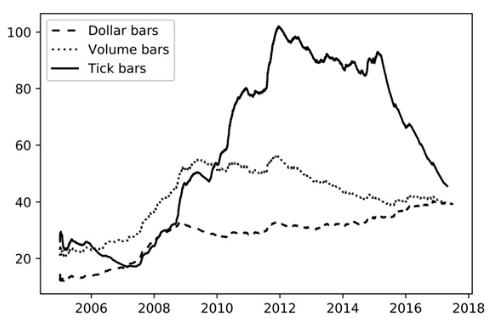
\includegraphics[scale=0.55]{figures/intro/standardbars}
\caption{Average daily frequency of tick, volume, and dollar bars}
\end{figure}

\begin{remark} \hlt{Standard BARS}\\
Method to transform a series of observations arriving at irregular frequency into a homogeneous series derived from regular sampling.
\begin{enumerate}[label=\roman*.]
\setlength{\itemsep}{0pt}
\item Time Bars: obtained by sampling information at fixed intervals. Information collected includes timestamp, volume-weighted average price (VWAP), open price, close price, high price, low price, volume etc.\\
To be avoided as markets do not process information at constant time interval. Time bars oversample information in low-activity periods and under-sample information in high-activity periods. Time bars exhibit poor statistical properties, i.e., serial correlation, heteroscedasticity, non-normality of returns.
\item Tick Bars: sample variables extracted each time a pre-defined number of transactions take place. Allows synchronisation of sampling with a proxy of information arrival.\\
Sampling as a function of trading activity creates returns closer to IID Normal (\cite{Thierry_Helyette_2000}). When constructing tick bars, to be aware of outliers, as many exchanges carry out auction at open and at close; order book accumulates bids and offers without matching. Order fragmentation introduces some arbitrariness in number of ticks. Matching engine protocols may split one fill into multiple artificial partial fills as a matter of operational convenience.
\item Volume Bars: samples every time a pre-defined amount of security's units that have been exchanged.\\
Achieves better statistical properties than sampling tick bars.\\
Convenient artefact for studying market microstructure theories.
\item Dollar Bars: samples an observation every time a pre-defined market value is exchanged. Used when the analysis involves significant price fluctuations. Robust against corporate actions such as splits, reverse splits, issuance of new shares, buying back existing shares.\\
Bar size could be dynamically adjusted as a function of free-floating market cap of a company or outstanding amount of issued debt.
\end{enumerate}
\end{remark}

\begin{remark} \hlt{Information-Driven Bars}\\
Method to sample more frequently when new (micro-structural) information arrives to the market.
\begin{enumerate}[label=\roman*.]
\setlength{\itemsep}{0pt}
\item Tick Imbalance Bars: sample bars whenever tick imbalance exceeds expectations. To determine tick index $T$ such that accumulation of signed ticks exceeds a given threshold.\\
Let $\{(p_t, v_t)\}_{t=1, \ldots, T}$ be sequence of ticks where $p_t$ and $v_t$ is the price and volume associated with tick $t$. Let tick rule define a sequence $\{b_t\}_{t=1, \ldots, T}$ where
\begin{align}
b_t = 
\begin{cases}
b_{t-1} \ \ \ \text{if } \Delta p_t = 0 \\
\frac{\abs{\Delta p_t}}{\Delta p_t} \ \ \text{if } \Delta p_t \neq 0
\end{cases} \nonumber
\end{align}
The tick imbalance at time $T$ is defined as 
\begin{equation}
\theta_T = \sum\limits_{t=1}^T b_t \nonumber
\end{equation}
Compute expected value of $\theta_T$ at beginning of the bar,
\begin{equation}
E_0[\theta_T] = E_0 [T](P[b_t = 1] - P[b_t = -1]) = E_0 [T](2P[b_t = 1] - 1) \nonumber
\end{equation}
where $E_0[T]$ is expected size of tick bar, $P[b_t = 1]$ and $P[b_t = -1]$ is unconditional probability that a tick is classified as a buy and sell. In practice, $E_0[T]$ and $(2P[b_t = 1] - 1)$ may be estimated as an exponentially weighted moving average of $T$ and $b_t$ values from prior bars.\\
Define the tick imbalance bar (TIB) as a $T^{*}$ contiguous subset of ticks such that
\begin{equation}
T^{*} = \arg \min_T \{ \abs{\theta_T} \geq E_0 [T] \ \vert \ 2 P[b_t = 1] - 1 \} \nonumber
\end{equation}
where the size of expected imbalance is implied by $\abs{2 P[b_t = 1] - 1}$.\\
When $\theta_T$ is more imbalanced than expected, a low $T$ will satisfy the conditions.\\
TIBs are produced more frequently under presence of informed trading (asymmetric information that triggers one-side trading). TIBs are buckets of trades containing equal amounts of information.
\item Volume/Dollar Imbalance Bars: sample bars when volume or dollar imbalances diverge from expectations.\\
First, define imbalance at time $T$ as
\begin{equation}
\theta_T = \sum\limits_{t=1}^T b_t v_t \nonumber
\end{equation}
where $v_t$ may represent ether number of securities traded (VIB) or dollar amount traded (DIB).\\
The expected value of $\theta_T$ at the beginning of the bar is then computed as
\begin{align}
E_0[\theta_T] &= E_0 \left[ \sum\limits_{t \vert b_t = 1}^T v_t \right] - E_0 \left[ \sum\limits_{t \vert b_t = -1}^T v_t \right] \nonumber \\
&= E_0[T] (P[b_t = 1]E_0[v_t \vert b_t = 1] - P[b_t = -1]E_0[v_t \vert b_t = -1]) \nonumber \\
&= E_0[T] (v^+ - v^-) \nonumber
\end{align}
where the initial expectation of $v_t$ is decomposed into component contributed by buys and sells. Then
\begin{equation}
E_0[\theta_T] = E_0[T] (2v^+ - E_0 [v_t]) \nonumber
\end{equation}
In practice, $E_0[T]$ and $(2v^+ - E_0 [v_t])$ may be estimated as exponentially weighted moving average of $T$ and $b_t v_t$ values from prior bars. Next, define VIB or DIB as a $T^*$-contiguous subset of ticks such that
\begin{equation}
T^* = \arg \min_T \{ \abs{\theta_T} \geq E_0[T] \ \vert \ 2v^+ - E_0[v_t] \} \nonumber
\end{equation}
where the size of expected imbalance is implied by $\abs{2v^+ - E_0[v_t]}$.\\
When $\theta_T$ is more imbalanced then expected, a low $T$ will satisfy the conditions.\\
VIB and DIB addresses concerns on tick fragmentation and outliers, and also addresses the issues of corporate actions, as the bar size is adjusted dynamically.
\item Tick Runs Bars: sample bars when the sequence of buys in overall volume diverges from expectations. For the case when large traders sweep order book, use iceberg orders, or slice parent orders into multiple children, all leaving a trace of runs in the $\{b_t\}_{t = 1, \ldots, T}$ sequence. Define length of current run as
\begin{equation}
\theta_T = \max \left\{ \sum\limits_{t \vert b_t = 1}^T b_t - \sum\limits_{t \vert b_t = -1}^T b_t  \right\} \nonumber
\end{equation}
The expected value of $\theta_T$ at beginning of bar is computed as
\begin{equation}
E_0[\theta_T] = E_0[T] \max \{P[b_t = 1], 1 - P[b_t = 1] \} \nonumber
\end{equation}
In practice, $E_0[T]$ and $P[b_t = 1]$ may be estimated as exponentially weighted moving average of $T$ and proportion of buy ticks from prior bars. Next, define TRB as $T^*$-contiguous subset of ticks such that
\begin{equation}
T^* = \arg \min_T \{ \theta_T \geq E_0[T] \max \{P[b_t = 1], 1 - P[b_t = 1] \} \} \nonumber
\end{equation}
where the expected count of ticks from runs is implied by $\max \{P[b_t = 1], 1 - P[b_t = 1] \}$.\\
When $\theta_T$ exhibits more runs than expected, a low $T$ will satisfy these conditions.\\
Instead of measuring length of longest sequence, count number of ticks of each side without offsetting.
\item Volume/Dollar Runs Bars: sample bars when volume or dollars traded by one side exceed expectation for a bar. First, define volume or dollars associated with a run as
\begin{equation}
\theta_T = \max \left\{ \sum\limits_{t \vert b_t = 1}^T b_t v_t - \sum\limits_{t \vert b_t = -1}^T b_t v_t \right\} \nonumber
\end{equation}
where $v_t$ may either represent volume (VRB) or dollar amount exchanged (DRB). The expected value of $\theta_T$ at beginning of the bar is then
\begin{align}
E_0 [\theta_T] = E_0[T] \max \{ P[b_t = 1]E_0[v_t \vert b_t = 1], (1 - P[b_t = 1]) E_0[v_t \vert b_t = -1] \} \nonumber
\end{align}
In practice, $E_0[T], P[b_t = 1], E_0[v_t \vert b_t = 1], E_0[v_t \vert b_t = -1]$ may be estimated as exponentially weighted moving average of $T$, proportion of buy ticks, buy volumes, and sell volumes from prior bars. Next, define a volume runs bar (VR) as $T^*$-contiguous subset of ticks such that
\begin{equation}
T^* = \arg \min_T \{ \theta_T \geq E_0[T] \max \{P[b_t = 1]E_0[v_t \vert b_t = 1], (1 - P[b_t = 1]) E_0[v_t \vert b_t = -1] \} \} \nonumber
\end{equation}
expected volume from runs is implied by $\max \{P[b_t = 1]E_0[v_t \vert b_t = 1], (1 - P[b_t = 1]) E_0[v_t \vert b_t = -1] \} \}$.\\
When $\theta_T$ exhibits more runs than expected, volume from runs is greater than expected, a low $T$ will satisfy these conditions.
\end{enumerate}
\end{remark}

\begin{definition} \hlt{Multi-Product Series: ETF Trick}\\
To model a basket of securities as if it was a single cash product. To transform any complex multi-product dataset into a single dataset that resembles a total return ETF.
\end{definition}

\begin{method} \hlt{ETF Trick}\\
Produce a time series that reflects the value of $\$1$ invested. Changes in the series will reflect changes in PnL, series will be strictly positive, and implementation shortfall will be taken into account. The bars contain:
\begin{enumerate}[label=\roman*.]
\setlength{\itemsep}{0pt}
\item Raw open price of instrument $i = 1, \ldots, I$ at bar $t = 1, \ldots, T$: $o_{i,t}$
\item Raw close price of instrument $i = 1, \ldots, I$ at bar $t = 1, \ldots, T$: $p_{i,t}$
\item USD value of one point of instrument $i = 1, \ldots, I$ at bar $t = 1, \ldots, T$: $\varphi_{i,t}$. This includes forex rate.
\item Volume of instrument $i = 1, \ldots, I$ at bar $t = 1, \ldots, T$: $v_{i,t}$
\item Carry, dividend, or coupon paid by instrument $i$ at bar $t$: $d_{i,t}$. Variable can also be used to charge margin costs or costs of funding.
\end{enumerate}
All instruments $i = 1, \ldots, I$ were tradable at bar $t = 1, \ldots, T$. Even if some instruments were not tradable over entirety of time interval $[t-1, t]$, at least they were tradable at times $t-1$ and $t$.\\
For basket of securities with allocation vector $\omega_t$ rebalanced (or rolled) on bars $B \subseteq \{1, \ldots, T \}$, the $\$1$ investment value $\{K_t\}$ is derived as 
\begin{align}
h_{i,t} &= 
\begin{cases}
\frac{\omega_{i,t} K_t}{o_{i, i+1} \varphi_{i,t} \sum\limits_{i=1}^I \abs{\omega_{i,t}}} \ \ \ \text{if } t \in B \\
h_{i, t - 1} \ \ \ \ \ \ \ \ \ \ \ \ \ \ \ \ \text{otherwise}
\end{cases} \nonumber \\
\delta_{i,t} &=
\begin{cases}
p_{i,t} - o_{i,t} \ \ \ \text{if } (t-1) \in B \\
\Delta p_{i,t} \ \ \ \ \ \ \ \ \ \ \ \ \ \ \ \ \ \text{otherwise}
\end{cases} \nonumber \\
K_t &= K_{t-1} + \sum\limits_{i=1}^I h_{i, t-1} \varphi_{i,t} (\delta_{i,t} + d_{i,t}) \nonumber
\end{align}
where $K_0 = 1$ is the initial AUM. Variable $h_{i,t}$ is the holdings of instrument $i$ at time $t$, $\delta_{i,t}$ is change of market value between $t-1$ and $t$ for instrument $i$. Note profits or losses are being reinvested whenever $t \in B$, hence preventing negative prices. Dividends $d_{i,t}$ are already embedded in $K_t$.\\
The purpose of $\omega_{i,t} \left( \sum_{i=1}^I \abs{\omega_{i,t}} \right)^{-1}$ is to de-lever the allocations.\\
Let $\tau_i$ be transaction cost associated with trading $\$1$ of the instrument. Three additional variables that the strategy needs to know for every observed bar $t$ are:
\begin{enumerate}[label=\roman*.]
\setlength{\itemsep}{0pt}
\item Rebalance Costs: variable cost $\{c_t\}$ associated with allocation rebalance is
\begin{equation}
c_t = \sum\limits_{i=1}^I (\abs{h_{i, t-1}}p_{i,t} + \abs{h_{i,t}} o_{i, t+1}) \varphi_{i,t} \tau_{i} \ \ \ \forall t \in B \nonumber
\end{equation}
Note $c_t$ is not embedded in $K_t$, as shorting will generate fictitious proceeds when allocation is rebalanced.\\
In code, $\{c_t\}$ is treated as a (negative) dividend.
\item Bid-Ask Spread: the cost $\{ \tilde{c}_t \}$ of buying or selling one unit of this ETF,
\begin{equation}
\tilde{c}_t = \sum\limits_{i=1}^I \abs{h_{i, t-1}}p_{i, t} \varphi_{i,t} \tau_i \nonumber
\end{equation}
When a unit is bought or sold, strategy must charge this cost $\tilde{c}_t$.
\item Volume: volume traded $\{v_t \}$ is determined by least active member in the basket. Let $v_{i,t}$ be volume traded by instrument $i$ over bar $t$. The number of tradable basket units is
\begin{equation}
v_t = \min_i \left\{ \frac{v_{i,t}}{\abs{h_{i, t-1}}} \right\} \nonumber
\end{equation}
\end{enumerate}
Transaction costs functions may not be linear, and can be simulated by the strategy.
\end{method}

\begin{method} \hlt{ETF Trick: Computation of Allocation Vector with PCA}\\
Consider an IID multivariate Gaussian process with means vector $\mu$ of size $N \times 1$, and covariance matrix $V$ of size $N \times N$. First, perform spectral decomposition $VW = W \Lambda$, where columns in $W$ are reordered so that elements of $\Lambda$ diagonal are sorted in descending order. Second, given allocations vector $\omega$, portfolio risk is
\begin{equation}
\sigma^2 = \omega' V \omega = \omega' W \Lambda W' \omega = \beta' \Lambda \beta = (\Lambda^{1/2} \beta)' (\Lambda^{1/2} \beta)' \nonumber
\end{equation}
 where $\beta$ is projection of $\omega$ on orthogonal basis. Third, $\Lambda$ is a diagonal matrix, thus
\begin{equation}
\sigma^2 = \sum\limits_{n=1}^N \beta^2_n \Lambda_{n,n} \nonumber
\end{equation}
The risk attributed to the $n$th component is
\begin{equation}
R_n = \beta^2_n \Lambda_{n,n}\sigma^{-2} = [W' n]^2_n \Lambda_{n,n} \sigma^{-2} \nonumber
\end{equation}
with $R' 1_N = 1$, and $1_N$ is a vector of $N$ ones.\\
Note $\{R_n\}_{n=1, \ldots, N}$ is distribution of risks across orthogonal components.\\
Next, compute vector $\omega$ which delivers user-defined risk distribution $R$. Note from earlier,
\begin{equation}
\beta = \left\{ \sigma \sqrt{\frac{R_n}{\Lambda_{n,n}}} \right\}_{n = 1, \ldots, N} \nonumber
\end{equation}
which represents allocation in new (orthogonal basis).\\
The allocation in old basis is $\omega = W \beta$. Rescaling $\omega$ re-scales $\sigma$, hence keeping risk distribution constant.
\end{method}

\begin{method} \hlt{ETF Trick: Single Futures Roll}\\
To work with non-negative rolled series, derive price series of $\$ 1$ investment as follows:
\begin{enumerate}[label=\roman*.]
\setlength{\itemsep}{0pt}
\item Compute time series of rolled futures prices
\item Compute return $r$ as rolled price change divided by previous roll price
\item Form a price series using these returns
\end{enumerate}
\end{method}

These methods allow us to produce a continuous, homogeneous, and structured dataset from collection of unstructured financial data. Note however, that several ML algorithms do not scale well with sample size. ML algorithms achieve higher accuracy when they attempt to learn from relevant examples.

\begin{method} \hlt{Sampling for Reduction}\\
To reduce the amount of data used to fit ML algorithm, downsampling could be used.
\begin{enumerate}[label=\roman*.]
\setlength{\itemsep}{0pt}
\item Sequential sampling at constant step size (linspace sampling)
\item Sampling randomly using uniform distribution (uniform sampling)
\end{enumerate}
Note both samples do not necessarily contain subset of most relevant observations.
\end{method}

\begin{method} \hlt{Event-Based Sampling: CUMSUM Filter} \\
Bets are often placed after some event takes place, hence to let ML algorithm learn whether there is an accurate prediction function under these circumstances, CUSUM filter could be used.\\
This is a quality-control method, to detect shift in mean value of measured quantity away from a target value.\\
Let $\{y_t\}_{t=1, \ldots, T}$ be IID observations arising from a locally stationary process. The cumulative sums are
\begin{equation}
S_t = \max \{0, S_{t-1} + y_t - E_{t-1} [y_t] \}, \ \ \ S_0 = 0 \nonumber
\end{equation}
An action will be recommended at the first $t$ satisfying $S_t \geq h$ for some threshold $h$ (filter size).\\
Note $S_t = 0$ whenever $y_t = E_{t-1}[y_t] - S_{t-1}$, The zero floor means some downward deviations will be skipped.\\
The filter is set up to identify a sequence of upside divergences from any reset level zero.\\
The threshold is activated when
\begin{equation}
S_t \geq h \Leftrightarrow \exists \tau \in [1, t] \ \vert \ \sum\limits_{i=\tau}^t (y_i - E_{i-1}[y_t]) \geq h \nonumber
\end{equation}
This concept of run-ups can be extended to include run-downs, giving symmetric CUSUM filter.
\begin{align}
S^+_t &= \max \{0, S^+_{t-1} + y_t - E_{t-1}[y_t] \}, \ \ \ S^+_0 = 0 \nonumber \\
S^-_t &= \min \{0, S^-_{t-1} + y_t - E_{t-1}[y_t] \}, \ \ \ S^-_0 = 0 \nonumber \\
S_t &= \max \{S^+_t, -S^-_t \} \nonumber
\end{align}
\end{method}

\subsubsection{Data Labelling Techniques}

\begin{method} \hlt{Labelling with Fixed-Time Horizon Method}\\
Given features matrix $X$ with $I$ rows, $\{X_i\}_{i = 1, \ldots, I}$ drawn from some bards with index $t = 1, \ldots, T$, where $I \leq T$, let an observation $X_i$ be assigned a label $y_i \in \{-1, 0, 1\}$,
\begin{align}
y_i &=
\begin{cases}
-1 \ \ \ \text{if } r_{t_{i,0}, t_{i,0} + h} < -\tau \\
0 \ \ \ \ \ \ \text{if } \abs{r_{t_{i,0}, t_{i,0} + h}} \leq \tau \\
1 \ \ \ \ \ \ \text{if } r_{t_{i,0}, t_{i,0} + h} > \tau
\end{cases} \nonumber \\
r_{t_{i,0}, t_{i,0} + h} &= \frac{p_{t_{i,0}+h}}{p_{t_{i,0}}} - 1 \nonumber
\end{align}
where $\tau$ is a pre-defined constant threshold, $t_{i,0}$ is index of bar immediately after $X_i$ takes place, $t_{i,0} + h$ is index of $h$-th bar after $t_{i,0}$, and $r_{t_{i,0}, t_{i,0} + h}$ is price return over bar horizon $h$.
\end{method}

\begin{remark} \hlt{Limitations of Fixed-Time Horizon Method}
\begin{enumerate}[label=\roman*.]
\setlength{\itemsep}{0pt}
\item Time bars do not exhibit good statistical properties (as seen earlier)
\item The same threshold $\tau$ is applied regardless of observed volatility.\\
Compute daily volatility at intraday estimation points, applying span of $n$ days t an exponentially weighted moving standard deviation.
\end{enumerate}
\end{remark}

\begin{method} \hlt{Labelling with Triple-Barrier Method}\\
Labels an observation according to first barrier touched out of three barriers.
\begin{enumerate}[label=\roman*.]
\setlength{\itemsep}{0pt}
\item Set two horizontal barriers and one vertical barrier. Horizontal barriers are defined by profit-taking and stop-loss limits, which are a dynamic function of estimated volatility (realised or implied). Third barrier is the number of bars elapsed since the position was taken (expiration limit).
\item If upper barrier is touched first, label observation as $1$. If lower barrier is touched first, label observation as $-1$. If vertical barrier is touched first, either label by sign of the return or with $0$.
\end{enumerate}
Note that the method is path-dependent. To label an observation, need to account for entire path spanning $[t_{i,0}, t_{i,0} + h]$ where $h$ defines the vertical barrier (expiration limit). Let $t_{i,1}$ be the time of first barrier touch with return as $r_{t_{i,0}, t_{i,1}}$. The horizontal barriers may not be symmetric.
\end{method}

\begin{remark} \hlt{Triple-Barrier Method Configurations}\\
Denote a barrier configuration by triplet $[pt, sl, t1]$ which are the upper barrier, lower barrier, physical barrier. Set value as $0$ if barrier is inactive, and $1$ if barrier is active.\\
The three useful configurations are:
\begin{enumerate}[label=\roman*.]
\setlength{\itemsep}{0pt}
\item $[1,1,1]$: to realise profit, but have set a maximum tolerance for losses and a holding period.
\item $[0,1,1]$: to exit after a number of bars, unless stopped-out.
\item $[1,1,0]$: take profit as long as not stopped-out.
\end{enumerate}
The three less realistic configurations are:
\begin{enumerate}[label=\roman*.]
\setlength{\itemsep}{0pt}
\item $[0,0,1]$: equivalent to fixed-time horizon method. 
\item $[1,0,1]$: position held until a profit is made or maximum holding period is exceeded, without regard for immediate unrealised losses
\item $[1,0,0]$: position is held until a profit is made. Could lock in loose position for years.
\end{enumerate}
The two illogical configurations are:
\begin{enumerate}[label=\roman*.]
\setlength{\itemsep}{0pt}
\item $[0,1,0]$: aimless. Hold position until stopped-out.
\item $[0,0,0]$: no barriers. Position locked forever, no label generated.
\end{enumerate}
\end{remark}

\begin{figure}[H]
\centering
\scalebox{0.75}{\input{figures/intro/metalabel.tikz}}
\caption{Meta-Labelling Process}
\end{figure}

\begin{method} \hlt{Meta-Labelling}\\
The technique is particularly helpful to achieve higher F1-scores.\\
First, build a model that achieves high recall, even if precision is not particularly high. Second, correct for low precision by applying meta-labelling to positives predicted by primary model.\\
Meta-labelling will filter out false positives, where majority of positives have been identified by primary model. The second model's purpose is to determine if the positive from primary model is true or false.
\begin{enumerate}[label=\roman*.]
\setlength{\itemsep}{0pt}
\item Train a primary model (binary classification)
\item A threshold level is determined at which the primary model has a high recall, ROC curves could be used to help determine a good level.
\item Typical features of second model are as follows:
\begin{enumerate}[label=\roman*.]
\setlength{\itemsep}{0pt}
\item Primary model features concatenated with predictions from first model.
\item Market state
\item Features indicative of false positives
\item Distribution related
\item Recent model performance
\end{enumerate}
Meta Labels are used as target variable in second model. Fit the second model
\item Prediction from the secondary model is combined with the prediction from the primary model and only where both are true, is your final prediction true.
\end{enumerate}
\end{method}

\begin{remark} \hlt{Limitations of Meta-Labelling}
\begin{enumerate}[label=\roman*.]
\setlength{\itemsep}{0pt}
\item If model has overfit the data, meta-labelling will not add much value
\item If every trade is not treated as an independent observation, the meta-model is forced to determine day-to-day exposures, which is the wrong way to apply the technique
\item Technique trades recall for precision. Require a large number of trades to train on, while being happy with reduction in trade frequency
\end{enumerate}
\end{remark}

\subsubsection{Data Sample Weights}

Note that most of ML literature is based on IID assumption, and ML applications usually fail in finance as these assumptions are unrealistic in the case of financial time series.

\begin{remark} \hlt{Overlapping Outcomes}\\
Let label $y_i$ be assigned to an observed feature $X_i$, where $y_i = f([t_{i,0}, t_{i,1}])$ is a function over the interval. When $t_{i,1} > t_{j,0}$ and $i < j$, then $y_j$ will depend on common return $r_{t_{j,0}, \min\{t_{i,1}, t_{j,1}\}}$ (over interval $[t_{j,0}, \min\{t_{i,1}, t_{j,1}\}]$). The series of labels $\{y_i \}_{i-1, \ldots, J}$ are not IID whenever there is overlap between any two consecutive outcomes, i.e., $\exists i \ \vert \ t_{i,1} > t_{i+1, 0}$. If this is resolved by restricting bet horizon to $t_{i,1} \leq t_{i+1, 0}$, there is no overlap, but this will lead to coarse models where features sampling frequency is limited by horizon used to determine outcome.\\
To investigate outcomes that lasted a different duration, samples have to be resampled with different frequency. In addition, if path-dependent labelling technique is to be applied, the sampling frequency will be subordinated to first barrier's touch. Hence, to use $t_{i,1} > t_{i+1, 0}$, leading to overlapping outcomes.
\end{remark}

\begin{method} \hlt{Estimating Uniqueness of Label}\\
Let two labels $y_i$ and $y_j$ be concurrent at time $t$, both a function of at least one common return $r_{t-1, t} = \frac{p_t}{p_{t-1}} = 1$.\\
To compute the number of labels that are a function of given return $r_{t-1, t}$:
\begin{enumerate}[label=\roman*.]
\setlength{\itemsep}{0pt}
\item For each $t = 1, \ldots, T$, form a binary array $\{1_{t,i}\}_{i=1, \ldots, I}$ where $1_{t, i} \in \{0,1 \}$.\\
Variable $1_{t,i} = 1$ if and only if $[t_{i,0}, t_{i,1}]$ overlaps with $[t-1, t]$ and $1_{t,i}=0$ otherwise.
\item Compute the number of labels concurrent at $t$, $c_t = \sum\limits_{i=1}^I 1_{t,i}$
\end{enumerate}
\end{method}

\begin{method} \hlt{Average Uniqueness of Label}\\
To estimate label's uniqueness (non-overlap) across its lifespan.
\begin{enumerate}[label=\roman*.]
\setlength{\itemsep}{0pt}
\item Uniqueness of label $i$ at time $t$ is $u_{t,i} = 1_{t,i} c^{-1}_{t}$.
\item Average uniqueness of label $i$ is average $u_{t,i}$ over label's lifespan, $\overline{u}_i = (\sum_{t=1}^T u_{t,i}) (\sum_{t=1}^T 1_{t,i})^{-1}$.
\end{enumerate}
Note that $\{\overline{u}_{i}\}_{i=1, \ldots, I}$ are not used for forecasting the label, hence there is no information leakage.
\end{method}

\begin{remark} \hlt{IID and Oversampling}\\
Probability of not selecting item $i$ after $I$ draws with replacement on set of $I$ items is $(1 - I^{-1})^I$. As $I \rightarrow \infty$, note that $(1 - I^{-1})^I \rightarrow e^{-1}$. Number of unique observations drawn to be expected is $(1- e^{-1}) \approx \frac{2}{3}$.\\
If maximum number of overlapping outcomes is $K \leq I$, probability of not selecting a particular item $i$ after $I$ draws with replacement on set of $I$ items is $(1 - K^{-1})^I$. As sample size increase, probability can be approximated as $(1-I^{-1})^{I \frac{K}{I}} \approx e^{-\frac{K}{I}}$. Implication is that incorrectly assuming IID draws lead to oversampling.
\end{remark}

\begin{method} \hlt{Sampling with Bootstrap, Redundancy}\\
Sampling with bootstrapping on observations where $I^{-1} \sum_{i=1}^{I} \overline{u}_i \ll 1$, in-bag observations will increasingly be redundant to each other, and very similar to out-of-bag observations. Two solutions may be:
\begin{enumerate}[label=\roman*.]
\setlength{\itemsep}{0pt}
\item Drop overlapping outcomes before performing bootstrap.\\
As overlaps are not perfect, dropping an observation due to overlap will lead to extreme loss in information.
\item Utilise the average uniqueness $I^{-1} \sum_{i=1}^{I} \overline{u}_i$ to reduce undue influence of outcomes that contain redundant information. Ensure in-bag observations are not sampled at frequency much higher than uniqueness.
\end{enumerate}
\end{method}

\begin{method} \hlt{Sequential Bootstrap}\\
Draws made according to changing probability that controls for redundancy.
\begin{enumerate}[label=\roman*.]
\setlength{\itemsep}{0pt}
\item Observation $X_i$ is drawn from uniform distribution, $i \sim U[1, I]$.\\
Probability of drawing any value $i$ is $\delta^{(1)}_i = I^{-1}$.
\item Second draw, to reduce probability of drawing observation $X_j$ with highly overlapping outcome.\\
Let $\varphi$ be sequence of draws (may include repetitions), where $\{\varphi^{(1)}\} = \{i\}$.\\
Uniqueness of $j$ at time $t$ is $u^{(2)}_{t,j} = 1_{t,j} (1 + \sum_{k \in \varphi^{(1)}} 1_{t,k})^{-1}$, which is the uniqueness from adding alternative $j$'s to existing sequence of draws $\varphi^{(1)}$.\\
Average uniqueness of $j$ is average $u^{(2)}_{t,j}$ over $j$'s lifespan, $\overline{u}^{(2)}_j = (\sum_{t=1}^T u_{t,j}) (\sum_{t=1}^T 1_{t,j})^{-1}$.\\
A second draw can be made based on updated probabilities $\{\delta^{(2)}_j\}_{j = 1, \ldots, I}$:
\begin{equation}
\delta^{(2)}_j = \overline{u}^{(2)}_j \left( \sum\limits_{k=1}^I \overline{u}^{(2)}_j \right)^{-1} \nonumber
\end{equation}
where $\sum_{j=1}^I \delta^{(2)}_j = 1$.
Do a second draw, update $\varphi^{(2)}$, and re-evaluate $\{\delta^{(3)}_j \}_{j=1, \ldots, I}$.
\item Process is repeated until $I$ draws have taken place.
\end{enumerate}
Process draws samples much close to IID, verified by increase in $I^{-1} \sum_{i=1}^I \overline{u}_i$.
\end{method}

\begin{method} \hlt{Weighting Observations by Uniqueness and Absolute Return}\\
Let labels be a function for return sign ($\{-1, 1\}$ for standard label, $\{0, 1\}$ for meta-label). The sample weights can be defined in terms of sum of attributed returns over event's life-span, $[t_{i,0}, t_{i,1}]$,
\begin{equation}
\tilde{w}_{i} = \abs{\sum\limits_{t = t_{i,0}}^{t_{i,1}} \frac{r_{t-1, t}}{c_t}}, \ \ \ w_t = \tilde{w}_{i} \left( \sum\limits_{j=1}^I \tilde{w}_j \right)^{-1} \nonumber
\end{equation}
where $\sum_{i=1}^I w_i = I$. The method weigh an observation as a function of absolute log returns that can be attributed uniquely to it. Lower returns should be assigned higher weights.
\end{method}

\begin{method} \hlt{Time Decay Weighting} \\
To let sample weights decay as new observations arrive.\\
Let $d[x] \geq 0 \ \forall x \in [0, \sum_{i=0}^I \overline{u}_i]$ be time-decay factors multiplying sample weights from earlier.\\
The final weight has no decay, $d[\sum_{i=1}^I \overline{u}_i] = 1$, and all other weights will adjust relative to that.\\
Let $c \in (-1, 1]$ be user-defined parameters that determines decay function as follows:
\begin{enumerate}[label=\roman*.]
\setlength{\itemsep}{0pt}
\item If $c \in [0,1]$, then $d[1] = c$ with linear decay
\item If $c \in (-1, 0)$, then $d[-c \sum_{i=1}^I \overline{u}_i] = 0$, with linear decay between $[-c \sum_{i=1}^I \overline{u}_i, \sum_{i=1}^I \overline{u}_i]$,\\
and $d[x] \ \forall x \leq -c \sum_{i=1}^I \overline{u}_i$.
\end{enumerate}
If given linear piecewise function $d = \max \{0, a + bx\}$, requirements are met by following boundary conditions:
\begin{enumerate}[label=\roman*.]
\setlength{\itemsep}{0pt}
\item $d = a + b \sum_{i=1}^I \overline{u}_i = 1 \Rightarrow a = 1 - b \sum_{i=1}^I \overline{u}_i$
\item Contingent on $c$:
\begin{enumerate}[label=\arabic*.]
\setlength{\itemsep}{0pt}
\item $d = a + b0 = c \Rightarrow b = (1-c) (\sum_{i=1}^I \overline{u}_i)^{-1} \ \ \forall c \in [0,1]$
\item $d = a - bc \sum_{i=1}^I \overline{u}_i = 0 \Rightarrow b = [(c+1) \sum_{i=1}^I \overline{u}_i]^{-1} \ \forall c \in (-1, 0)$
\end{enumerate}
\end{enumerate}
In the implementation, decay takes place according to cumulative uniqueness. Note that
\begin{enumerate}[label=\roman*.]
\setlength{\itemsep}{0pt}
\item $c=1$ means there is no time decay
\item $0 < c < 1$ means weights decay linearly over time, but every observation still receives strictly positive weight, regardless of age
\item $c = 0$ means weights converge linearly to zero over time
\item $c < 0$ means oldest portion $cT$ of observations receive zero weight (erased from memory)
\end{enumerate}
\end{method}

\begin{method} \hlt{Class Weighting}\\
Weights for underrepresented labels. Critical in classification problems where the most important classes have rare occurrences. To assign higher weights to samples associated with those rare labels.
\end{method}

\subsubsection{Fractionally Differentiated Features}

Standard stationarity transformations (i.e. integer differentiation) reduce signal by removing memory. Although stationarity is necessary for inferential purposes, it is rarely the case that we want all memory to be erased.\\
Fractionally differentiated processes exhibit long-term persistence and anti-persistence, hence enhancing the forecasting power compared to standard ARIMA approach.

\begin{definition} \hlt{BackShift Operator}\\
Let $B$ be the backshift operator applied to a matrix of real-valued features $\{X_t \}$, where $B^k X_t = X_{t-k}$ for any integer $k \geq 0$. By binomial expansion, we then have
\begin{align}
(1-B)^d = \sum\limits_{k=0}^{\infty} \binom{d}{k} (-B)^k &= \sum\limits_{k=0}^{\infty} \prod\limits_{i=0}^{k-1} (d-i) \frac{(-B)^k}{k!} = \sum\limits_{k=0}^{\infty} (-B)^k \prod\limits_{i=0}^{k-1} \frac{d-i}{k-i} \nonumber \\
&= 1 - dB + \frac{d(d-1)}{2!} B^2 - \frac{d(d-1)(d-2)}{3!} B^3 + \cdots \nonumber 
\end{align}
\end{definition}

\begin{remark}
\label{rmk:propfracdifffeat} 
\hlt{Properties of Fractionally Differentiated Features}\\
Let $d$ be a real (non-integer) positive number. The arithmetic series consists of dot product
\begin{align}
\tilde{X}_t &= \sum\limits_{k=0}^{\infty} \omega_k X_{t-k} \nonumber \\
\omega &= \left\{ 1, -d, \frac{d(d-1)}{2!}, - \frac{d(d-1)(d-2)}{3!}, \ldots, (-1)^k \prod\limits_{i=0}^{k-1} \frac{d-1}{k!}, \ldots \right\} \nonumber \\
X &= \{X_t, X_{t-1}, \ldots, X_{t-k}, \ldots \} \nonumber
\end{align}
where $\omega$ are the weights, $X$ are the values. Properties of these features are:
\begin{enumerate}[label=\roman*.]
\setlength{\itemsep}{0pt}
\item Long memory: if $d$ is a positive integer number, then
\begin{equation}
\prod\limits_{i=0}^{k-1} \frac{d-i}{k!} = 0 \ \ \forall > d \nonumber
\end{equation}
and memory beyond that point is cancelled.
\item Iterative weight generation: given sequence of weights $\omega$, for $k = 0, \ldots, \infty$, the weights are
\begin{equation}
\omega_k = - \omega_{k-1} \frac{d - k + 1}{k}, \ \ \ \omega_0 = 1 \nonumber
\end{equation}
\item Convergence: For $k > d$, if $\omega_{k-1} \neq 0$, then
\begin{equation}
\abs{\frac{\omega_{k}}{\omega_{k-1}}} = \abs{\frac{d-k+1}{k}} < 1 \nonumber
\end{equation}
and $\omega_k = 0$ otherwise. Hence weights converge asymptotically to zero.\\
For positive $d$ and $k < d+1$, then $\frac{d-k+1}{k} \geq 0$, which makes initial weights alternate in sign.\\
For non-integer $d$, once $k \geq d+1$, $\omega_k$ will be negative if int$[d]$ is even, and positive otherwise.\\
In summary, $\lim_{k \rightarrow \infty} = 0^-$ when int$[d]$ is even, and $\lim_{k \rightarrow \infty} = 0^+$ when int$[d]$ is odd.\\
In special case $d \in (0,1)$, that $-1 < \omega_k < 0 \ \forall k > 0$. Alternate weight signs makes $\{\tilde{X}_t \}_{t = 1, \ldots, T}$ stationary, as memory wanes or is offset over the long run.
\end{enumerate}
\end{remark}

\begin{figure}[H]
\centering
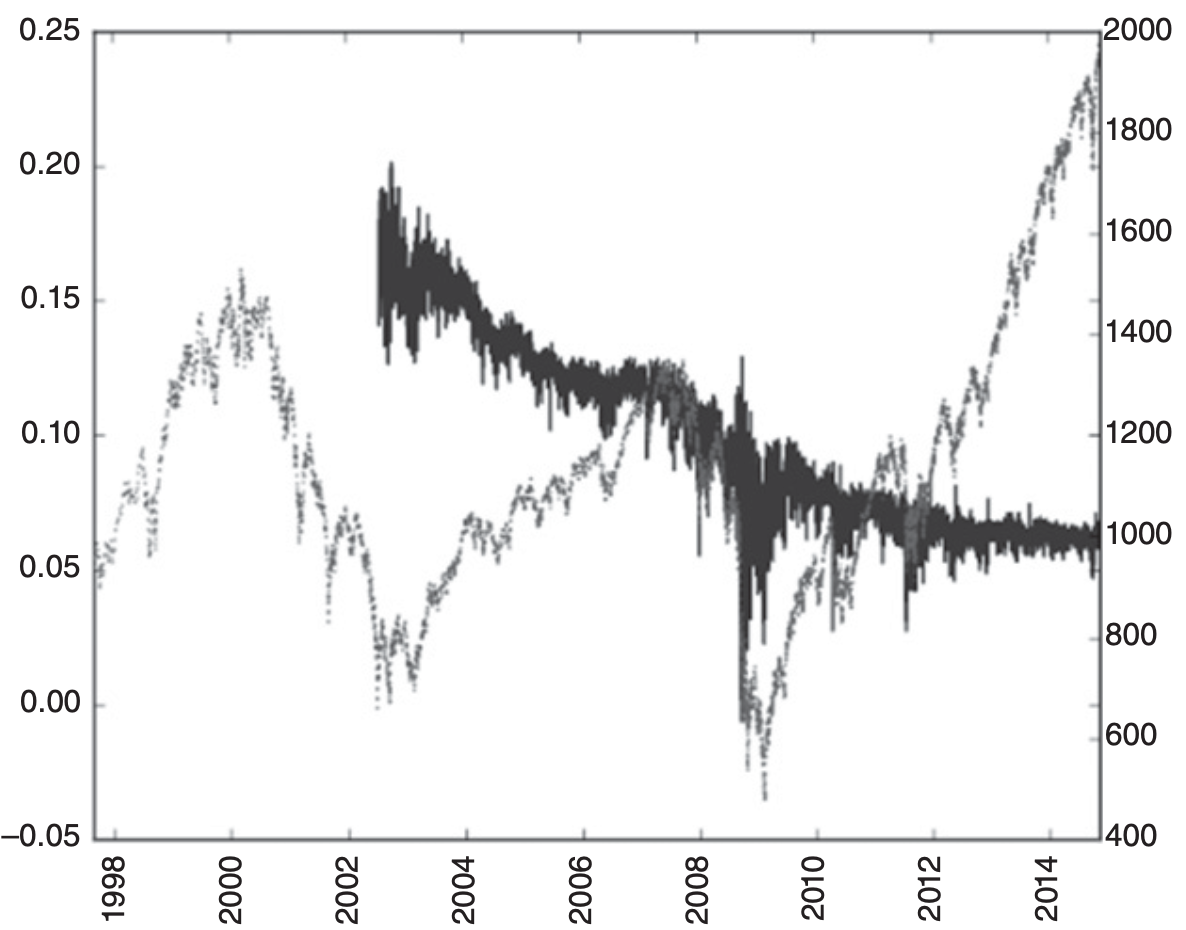
\includegraphics[scale=0.35]{figures/intro/fracdiffexpandwindow}
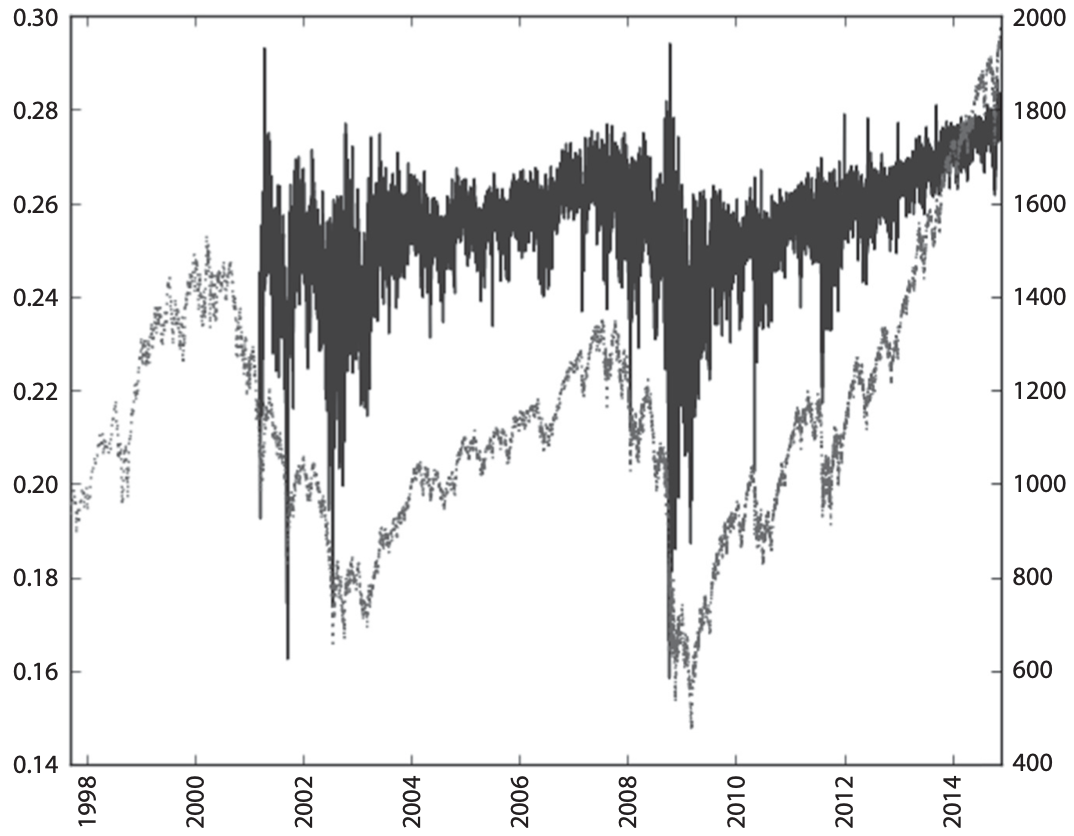
\includegraphics[scale=0.385]{figures/intro/fracdifffixedwidthwind}
\caption{Fractional differentiation controlling for weight loss with expanding and fixed-width window}
\end{figure}

\begin{method} \hlt{Expanding Window}\\
Given time series $T$ with real observations $\{X_t\}_{t = 1, \ldots, T}$, for each $l$, the relative weight loss is defined as
\begin{equation}
\lambda_l = \sum\limits_{j=T-l}^T \abs{\omega_j} \Bigg/ \sum\limits_{i=0}^{T-1} \abs{\omega_i} \nonumber
\end{equation}
Given tolerance level $\tau \in [0,1]$, determine value $l^*$ such that $\lambda_{l^*} \leq \tau$ and $\lambda_{l^* + 1} > \tau$. This value $l^*$ corresponds to the first results $\{\tilde{X}_t \}_{t = 1, \ldots, l^*}$, where weight-loss is beyond acceptable threshold $\lambda_t > \tau$.\\
From Remark \ref{rmk:propfracdifffeat}, it is clear $\lambda_{l^*}$ depends on convergence speed of $\{\omega_k \}$, which in turn depends on $d \in [0,1]$.\\
For $d = 1, \omega_k = 0 \ \forall k > 1$, and $\lambda_l = 0 \ \forall l > 1$, hence it suffices to drop $\tilde{X}_1$.\\
As $d \rightarrow 0^+$, $l^*$ increases, and larger portion of initial $\{\tilde{X}_t \}_{t = 1, \ldots, l^*}$ needs to be dropped to keep the weight loss $\lambda_{l^*} < \tau$. Note that there will be negative drift caused by negative weights added to initial observations as window is expanded. By controlling for weight loss, negative drift is still substantial as $\{\tilde{X}_t \}_{t = l^* + 1, \ldots, T}$ are computed on an expanding window.
\end{method}

\begin{method} \hlt{Fixed-Width Window}\\
Drop weights after their modulus $\abs{\omega_k}$ decreases below a given threshold $\tau$. This is equivalent to finding the first $l^*$ such that $\abs{\omega_{l^*}} \geq \tau$ and $\abs{\omega_{l^* + 1}} \leq \tau$, setting a new variable $\tilde{\omega}_k$:
\begin{align}
\tilde{\omega_k} = 
\begin{cases}
\omega_k \ \ \ \ \text{if } k \leq l^* \\
0 \ \ \ \ \ \ \text{if } k > l^*
\end{cases}, \ \ \ \ \
\tilde{X}_t = \sum\limits_{k=0}^{l^*} \tilde{\omega}_k X_{t-k} \ \ \text{for } t = T- l^* + 1, \ldots, T \nonumber
\end{align}
Note that the same vector of weights is used across all estimates of $\{\tilde{X}_t \}_{t = l^*, \ldots, T}$, hence avoiding negative drift caused by expanding window's added weights.\\
Distribution has skewness and excess kurtosis from memory, but it is stationary.
\end{method}


    
\newpage
   
\begin{comment}
	
% Mathematical and Statistical Foundation
    
    Adapted from materials such as Shreve’s stochastic calculus texts and advanced statistics references)

Stochastic Processes and Bayesian Inference:
Topics: Stochastic calculus, Markov processes, Bayesian linear regression, MCMC methods.
Purpose: Equip readers with rigorous tools to model market randomness and update beliefs with new data.
Optimization Techniques:
Topics: Convex optimization, dynamic programming, optimal control theory.
Purpose: Provide the mathematical underpinnings for optimal execution and risk management.
	
	% Quantitative Finance Theory
	(Incorporating insights from market microstructure texts and execution research)

Market Microstructure and Optimal Execution:
Topics: Order flow, transaction cost analysis, smart order routing, and alpha profiling.
Example: Discuss methods like VWAP, TWAP, and implementations from scholarly articles and Wikipedia’s smart order routing overview 
EN.WIKIPEDIA.ORG
.
Derivative Pricing and Risk Management:
Topics: Option pricing models, risk-adjusted cost functions, and sensitivity analysis.
Purpose: Bridge the gap between theoretical pricing models and their algorithmic application.

	% Algorithmic Trading Strategies
	(Drawing on works such as Michael Halls Moore’s “Advanced Algorithmic Trading” 
SACREDTRADERS.COM
and Ernie Chan’s insights)

Strategy Design and Testing:
Mean reversion, momentum, delta-neutral and statistical arbitrage strategies.
Detailed discussion of backtesting pitfalls and strategy decay.
Execution Algorithms:
In-depth treatment of execution strategies including slicing orders, smart order routing, and adaptive algorithms.
Case Studies:
Real-world examples (e.g., pairs trading with cointegration and Kalman filtering) that show the evolution from theoretical model to live trading.

	% Machine Learning and AI in Trading
	(Incorporating insights from “Advances in Financial Machine Learning” by Lopez de Prado
ANALYZINGALPHA.COM
 and related texts)

Supervised and Unsupervised Techniques:
Regression, decision trees, clustering, and support vector machines applied to financial data.
Deep Learning and Reinforcement Learning:
Neural networks for pattern recognition and forecasting, including practical coding examples in Python.
Feature Engineering and Model Evaluation:
Techniques for constructing and validating predictive models, with an emphasis on avoiding overfitting in a trading context.

	% Implementation, Backtesting, and Deployment
	(Using open-source tools like QSTrader, Python, and R – as highlighted in QuantInsti’s advanced courses 
QUANTRA.QUANTINSTI.COM
)

Efficient Backtesting Techniques:
Vectorized and event-driven backtesting frameworks.
Risk and Performance Metrics:
Detailed analysis of performance, risk-adjusted returns, and practical considerations when moving to live execution.
Real-Time Deployment:
Integrating machine learning models with live data streams, execution engines, and risk management systems.

	% Advanced Topics and Future Directions
	Emerging Trends:
Discussion on topics such as high-frequency trading (HFT) infrastructure, smart order routing, and dark pool strategies.
Reference recent research and articles (e.g., the “mundane economics” of HFT ).
Regulatory and Market Implications:
How evolving market regulations impact algorithm design and execution.

	% Appendices and Supplemental Materials
	Mathematical Proofs and Derivations:
Detailed proofs for key results for those interested in the theory.
Code Libraries and Examples:
Fully annotated code snippets (Python/R) that implement the discussed algorithms.
Glossary and Further Reading:
A curated list of additional resources and advanced texts (referencing lists from QuantInsti and other curated guides 
BLOG.QUANTINSTI.COM
).

    % Mathematical Overview Section
    \newpage
    %\section{Mathematical and Statistical Foundation}

An overview of the following fields of math:
\begin{enumerate}[label=\roman*.]
\setlength{\itemsep}{0pt}
\item Time Series Analysis
\item Stochastic Processes
\item Machine Learning
\end{enumerate}

This section serves as a guide in providing the fundamental knowledge required.

\subsection{Time Series Analysis}

Based on the books by James Douglas \cite{hamilton_1994}, and ...

\subsubsection{Stationary Time Series}

\begin{definition}
A \hlt{linear first-order difference equation} is defined as
\begin{equation}
y_t = \phi y_{t-1} + w_t \nonumber
\end{equation}
where $y_t$ is the target variable (with $y_{t-1}$ the lag $1$ variable), $w_t$ is an input variable at time $t$
\end{definition}

The difference equation may be solved by recursive substitution to arrive at
\begin{equation}
y_t = \phi^{t+1}y_{-1} + \phi^{t} w_0 + \phi^{t-1} w_1 + \phi^{t-2} w_2 + \cdots + \phi w_{t-1} + w_t \nonumber
\end{equation}

The \hlt{dynamic multiplier} calculates effect of $w_t$ on $y_{t+j}$, and is given by
\begin{equation}
\frac{\partial y_{t+j}}{\partial w_t} = \phi^j \nonumber
\end{equation}
If $\abs{\phi} < 1$, the system is stable. If $\abs{\phi} > 1$, then the system is explosive.

We may generalise the process to \hlt{$p$-th order difference equation}, i.e.,
\begin{equation}
y_t = \phi_t y_{t-1} + \phi_2 t_{t-2} + \cdots + \phi_p y_{t-p} + w_t \nonumber
\end{equation}
We may rewrite this as a first-order difference equation in a ($p \times 1$) vector $\bm{\xi}_t$:
\begin{equation}
\bm{\xi}_t = 
\begin{bmatrix}
y_t \\
y_{t-1} \\ 
\vdots \\
y_{t-p+1}
\end{bmatrix} \nonumber
\end{equation}
Define the ($p \times p$) matrix $\bm{F}$ by
\begin{equation}
\bm{F} =
\begin{bmatrix}
\phi_1 & \phi_2 & \phi_3 & \cdots & \phi_{p-1} & \phi_p \\
1 & 0 & 0 & \cdots & 0 & 0 \\
0 & 1 & 0 & \cdots & 0 & 0 \\
\vdots & \vdots & \vdots & \ddots & \vdots & \vdots \\
0 & 0 & 0 & \cdots & 1 & 0
\end{bmatrix} \nonumber
\end{equation}
Finally, define the ($p \times 1$) vector $\bm{v}_t$ by
\begin{equation}
\bm{v}_t =
\begin{bmatrix}
w_t \\
0 \\
0 \\
\vdots \\
0
\end{bmatrix} \nonumber
\end{equation}
Then the system of $p$ equations $\bm{\xi}_t = \bm{F} \bm{\xi}_{t-1} + \bm{v}_t$ is identical to the first order difference equation, and by recursive substitution, we have the following for the case of $p$-th order difference equation:
\begin{equation}
\bm{\xi}_{t + j} = \bm{F}^{j+1} \bm{\xi}_{t-1} + \bm{F}^{j} \bm{v}_{t} + \bm{F}^{j-1} \bm{v}_{t+1} + \cdots + \bm{F} \bm{v}_{t+j-1} + \bm{v}_{t+j} \nonumber
\end{equation}
Hence the dynamic multiplier is then $\frac{\partial y_{t+j}}{\partial w_t} f^{(j)}_{11}$, where $f^{(j)}_{11}$ is the $(1,1)$ element of $\bm{F}^j$.

\subsubsection{Univariate Time Series Models}

Trading activities through an exchange can be described by a sequence of time stamps ('ticks') $t_0 < t_1 < \cdots < t_n$, and 'marks' $y_i$ at time $t_i$, where $t_i$ denote market open, $t_n$ denote market close. The marks $y_i$ is a characteristic of the order book at time of $i$th activity. Events with marks associated with the ticks can be described mathematically as a marked point process.
\begin{figure}[H]
\centering
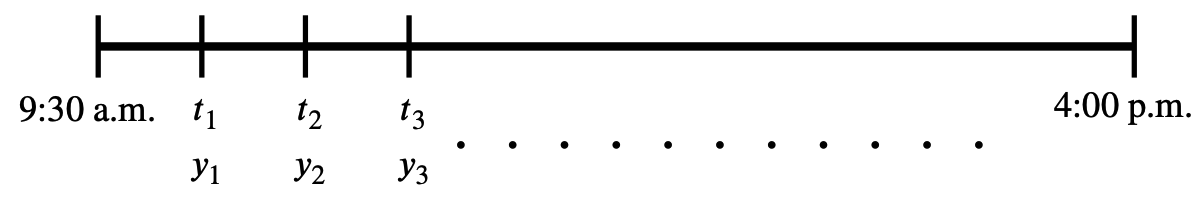
\includegraphics[scale=0.4]{images/math/tsa/ticksandmarks}
\caption{Ticks and Marks}
\end{figure}

A data aggregation method is where aggregation is conducted when there is a change in marker. An alternative aggregation method would be to divide the time span $T$ for exchange hours into $K$ intervals, so regularly spaced intervals are of size $\Delta t = T/K$. The time series method to be discussed will apply to all aggregated data.\\

Let $p_{it} = \ln P_{it}$ denote price of $i$th asset at time $t$; $p_t = (p_{1t}, p_{2t}, \ldots, p_{nt})$ denote price vector for $n$ assets; $y_{it}$ denote vector of characteristics of $i$th asset at time $t$. These quantities are aggregated from high frequency data. Consider $r$ factors $f_t = (f_{1t}, f_{2t}, \ldots, f_{rt})$ that may include market and industry factors, and asset characteristics. Trading rules can be broadly grouped as follows:
\begin{enumerate}[label=\roman*.]
\setlength{\itemsep}{0pt}
\item \hlt{Statistical Arbitrage}: $E(p_{i, t+1} \ \vert \ p_{i,t}, p_{i, t-1}, \ldots, y_{i,t}, y_{i, t-1}, \ldots)$, that predicts the price of $i$th stock at $t+1$ based on past trading information (also known as time series momentum)
\item \hlt{Momentum}: $E(p_{t+1} \ \vert \ p_t, p_{t-1}, \ldots, y_t, y_{t-1}, \ldots)$, that predicts the cross-sectional momentum of a subset of stocks based on past trading characteristics. For portfolio formation and rebalancing, pairs trading
\item \hlt{Fair Value}: $E(p_{t+1} \ \vert \ p_{t}, p_{t-1}, \ldots, y_t, y_{t-1}, \ldots, f_t, f_{t-1}, \ldots)$, predicts price using all relevant quantities. Factors normally include market, Fama-French; at a more macro level than timescale considered for price prediction, but may still be useful.
\end{enumerate}

Hence price and volatility prediction can be formulated as a time series prediction problem. Autocorrelations and partial autocorrelations can be used to build autoregressive and ARCH models with some predictive power.\\

Let $Y_1, Y_2, \ldots, Y_T$ be a sequence of random variables with a joint probability distribution. A sequence of observations of stochastic process $\{Y_t, t = 1, \ldots, T\}$ is a realisation of the process.\\
A time series $\{Y_t\}$ is \hlt{stationary} if for every integer $m$, the set of variables $Y_{t_1}, Y_{t_2}, \ldots, Y_{t_m}$ depends only on the distance between times $t_1, t_2, \ldots, t_m$. Thus $E(Y_t) = \mu$, $Var(Y_t) = \sigma^2$ are constant for all $t$.\\
The \hlt{auto-covariance} function is defined as
\begin{equation}
\gamma(s) = Cov(Y_t, Y_{t-s}) = E[(Y_t - \mu)(Y_{t-s} - \mu)] \ \ \forall s = 0, \pm 1, \ldots \nonumber
\end{equation}
The \hlt{auto-correlation} of process at lag $s$ is defined as
\begin{equation}
\rho(s) = Corr(Y_t, Y_{t-s}) = \frac{Cov(Y_t, Y_{t-s})}{\left(Var(Y_t) \ Var(Y_{t-s}) \right)^{1/2}} = \frac{\gamma(s)}{\gamma(0)}, \ \ \ \forall s = 0, \pm 1, \ldots \nonumber
\end{equation}

Some examples of stationary stochastic processes are as follows:

\begin{example} \hlt{(White Noise)} Sequence of discrete independent random variables (r.v.) $\{\epsilon_t \}$ with $E[\epsilon_t] = 0$ and $E[\epsilon_t^2] = \sigma^2$. Set $Y_t = \mu + \epsilon_t$, then $E[Y_t] = \mu$, $Cov(Y_t, Y_{t-s}) = Var(Y_t) = \sigma^2$ if $s=0$, and $Cov(Y_t, Y_{t-s}) = 0$ if $s \neq 0$. Hence the process is stationary.
\end{example}

\begin{example} \hlt{(Moving Average)} Let $\{\epsilon_t\}$ be independent r.v., with process $\{Y_t\}$ where $Y_t = \mu + \epsilon_t + \epsilon_{t_1}$ for $t = 0, 1, 2, \ldots$, and $\mu$ is constant. Then $E[Y_t] = \mu \ \forall t$, and
\begin{equation}
Cov(Y_t, Y_{t-s}) = \gamma(s) = 
\begin{cases}
2 \sigma^2 \ \ \text{if } s = 0 \\
\sigma^2 \ \ \text{if } s = 1 \\
0 \ \ \text{if } s > 1
\end{cases} \nonumber
\end{equation}
Hence $\{Y_t\}$ is stationary, with $\rho(s) = \gamma(s) / \gamma(0)$ such that $\rho(0) = 1$, $\rho(1) = 1/2$, $\rho(s) = 0$ for $\abs{s} > 1$.
\end{example}

Some examples of non-stationary stochastic processes are as follows:

\begin{example} \hlt{(Random Walk with Drift)} Let $\{\epsilon_t \}$ be sequence of independent r.v. with  $E[\epsilon_t] = 0$, $E[\epsilon_t^2] = \sigma^2$, and define process $\{Y_t\}$ by $Y_t = Y_{t-1} + \delta + \epsilon_t$ with $Y_0 = 0$. Then the process can be summarised as
\begin{equation}
Y_t = \delta t + \sum\limits_{j=1}^t \epsilon_j \nonumber
\end{equation}
Note that $E[Y_t] = \delta t$ and $Var[Y_t] = t \sigma^2$, hence process $\{Y_t\}$ is not stationary.
\end{example}

Given $T$ observations from stationary process $\{Y_t\}$, the \hlt{sample mean} is $\overline{Y} = \frac{1}{T} \sum\limits_{t=1}^T Y_t$. The \hlt{sample auto-covariance} function is defined by $\hat{\gamma}(s) = \frac{1}{T} \sum\limits_{t=1}^{T-s} (Y_t - \overline{Y})(Y_{T-s} - \overline{Y})$ for $s=0, 1, \ldots$. The \hlt{sample auto-correlation} function (ACF) is defined as $\hat{\rho}(s) = \frac{\hat{\gamma}(s)}{\hat{\gamma}(0)} = r(s)$. The \hlt{sample variance} is $Var(\overline{Y}) = \frac{\gamma(0)}{T}\left[1 + 2 \sum\limits_{u=1}^{Y-1} \left(\frac{T-u}{T} \right) \rho(u) \right]$; note that it has to account for auto-correlations.

\begin{definition} A stochastic process $\{Y_t\}$ is a \hlt{linear process} if it can be represented as
\begin{equation}
Y_t = \mu + \sum\limits_{j=0}^{\infty} \Psi_j \epsilon_{t-j} \nonumber
\end{equation}
where $\epsilon_t$ are independent with mean $0$, variance $\sigma_{\epsilon}^2$, and $\sum\limits_{j=0}^{\infty} < \infty$.
\end{definition}




\newpage

\subsection{Classical Machine Learning}

\subsubsection{Ensemble Methods}










\newpage

\subsection{Deep Learning}

\subsubsection{Deep Feedforward Networks}

\begin{remark} \hlt{Deep Feedforward Networks (DFNs)}\\
Defines a mapping $\bm{y} = f(\bm{x}; \bm{\theta})$ and learns value of parameters $\bm{\theta}$ that results in best function approximation.
\end{remark}

\begin{remark} \hlt{Linear Models}\\
Linear models may fit data efficiently and reliably, either in closed form or with convex optimisation.\\
Model capacity limited to linear functions, does not model interaction between any two input variables
\end{remark}

\begin{remark} \hlt{Nonlinear Models}\\
To represent nonlinear functions of $\bm{x}$, apply linear model to transformed input $\phi(\bm{x})$ where $\phi$ is a nonlinear transformation. Kernel trick may be applied to obtain nonlinear learning algorithm. To choose mapping $\phi$:
\begin{enumerate}[label=\roman*.]
\setlength{\itemsep}{0pt}
\item Choose generic $\phi$, such as that used by kernel machines based on RBF kernel.\\
If $\phi(\bm{x})$ is of high enough dimension, can find enough capacity to fit training set, but generalisations to test set remains poor. Mappings are based on principle of local smoothness and do not encode enough prior information to solve advanced problems.
\item Manually engineer $\phi$. Requires decades of human effort for each task, and practitioners specialising in different domains (i.e, speech recognition, computer vision) with little transfer between domains.
\item Learn $\phi$ through deep learning. Model is $y = f(\bm{x}; \bm{\theta}, \bm{w}) = \phi(\bm{x}; \bm{\theta})^T \bm{w}$, where parameters $\bm{\theta}$ can be used to learn $\phi$ from broad class of functions, and parameters $\bm{w}$ that map from $\phi(\bm{x})$ to desired output.\\
Do not require training problem to be convex, and only require finding the right general function.
\end{enumerate}
\end{remark}

\begin{definition} \hlt{Cost Functions}
\begin{enumerate}[label=\roman*.]
\setlength{\itemsep}{0pt}
\item Learning Conditional Distributions with Maximum Likelihood: cost function is negative log-likelihood, which is the cross-entropy between training data and model distribution:
\begin{equation}
J(\bm{\theta}) = - \mathbb{E}_{\bm{x}, \bm{y} \sim \hat{p}_{\text{data}}} \log p_{\text{model}}(\bm{y} \ \vert \ \bm{x}) \nonumber
\end{equation}
Specific form of cost function changes from model to model, depending on form of $\log p_{\text{model}}$.\\
Method removes the burden of designing cost functions for each model, as specifying a model $p(\bm{y} \ \vert \ \bm{x})$ automatically determines a cost function $\log p(\bm{y} \ \vert \ \bm{x})$.\\
Gradient of cost function for neural networks must be large and predictable enough to serve as good guide for the learning algorithm. The negative log-likelihood helps to avoid saturation of the function.
\item Learning Conditional Statistics: to learn just one conditional statistic of $\bm{y}$ given $\bm{x}$.\\
With sufficiently powerful neural network, this can represent any function $f$ from a wide class of function, limited by features of continuity and boundedness. Hence the cost function is a functional. Learning is choosing a functional rather than a set of parameters.\\
By calculus of variation	, solving the optimisation problem yields the below function,
\begin{align}
f^* &= \arg \min_f \mathbb{E}_{\bm{x}, \bm{y} \sim p_{\text{data}}} \Vert \bm{y} - f(\bm{x}) \Vert^2 \nonumber \\
f^* &= \mathbb{E}_{\bm{y} \sim p_{\text{data}}(\bm{y} \ \vert \ \bm{x})} [\bm{y}] \nonumber
\end{align}
If infinitely many samples from the true data-generating distribution could be trained, then minimising the mean squared error cost function gives a function that predicts mean of $\bm{y}$ for each value of $\bm{x}$.\\
A second result from calculus of variations is:
\begin{align}
f^* = \arg \min_f \mathbb{E}_{\bm{x}, \bm{y} \sim p_{\text{data}}} \Vert \bm{y} - f(\bm{x}) \Vert_1 \nonumber
\end{align}
which is a function that predicts the median value of $\bm{y}$ for each $\bm{x}$. This is the mean absolute error.\\
Note that mean squared error and mean absolute error often lead to poor results when used with gradient-based optimisation. Output units that saturate may produce very small gradients when combined with these cost functions. Hence the reason that cross-entropy cost function is more popular.
\end{enumerate}
\end{definition}

\begin{definition} \hlt{Output Units}
\begin{enumerate}[label=\roman*.]
\setlength{\itemsep}{0pt}
\item Linear Units: base on affine transformation with no nonlinearity.\\
Given features $\bm{h}$, a layer of output units produces vector $\hat{\bm{y}} = \bm{W}^T \bm{h} + \bm{b}$. Linear output layers are used to produce mean of conditional Gaussian distribution:
\begin{equation}
p(\bm{y} \ \vert \ \bm{x}) = \mathcal{N}(\bm{y}; \hat{\bm{y}}, \bm{I}) \nonumber
\end{equation}
Maximising log-likelihood is equivalent to minimising mean squared error.\\
Linear units do not saturate, hence may be used for wide variety of optimisation algorithms.
\item Sigmoid Units: define Bernoulli distribution $y$ conditioned on $\bm{x}$. Neural net to predict $P(y = 1 \ \vert \ \bm{x})$, which lies in interval $[0,1]$. The sigmoid unit is defined by
\begin{equation}
\hat{y} = \sigma(\bm{w}^T \bm{h} + b) \nonumber
\end{equation}
where $\sigma$ is the logistic sigmoid function.\\
Note that the cost function used with maximum likelihood is $- \log P(y \ \vert \ \bm{x})$, preventing saturation.\\
The loss function for MLE of Bernoulli parametrised by sigmoid is
\begin{equation}
J(\bm{\theta}) = - \log P(y \ \vert \ \bm{x}) = - \log \sigma((2y - 1)z) = \zeta((1-2y)z) \nonumber
\end{equation}
Function saturates only when $(1-2y)z$ is very negative, i.e., when model has the right answer.
\item Softmax Units: used to represent probability distribution over $n$ different classes.\\
A linear layer predicts unnormalised log probabilities:
\begin{equation}
\bm{z} = \bm{W}^T \bm{h} + \bm{b} \nonumber
\end{equation}
where $z_i = \log \tilde{P}(y=i \ \vert \ \bm{x})$. Softmax function is then
\begin{equation}
\text{softmax}(\bm{z})_i = \frac{\exp(z_i)}{\sum_j \exp(z_j)} \nonumber
\end{equation}
The function is to maximise $\log P(y=i ; \bm{z}) = \log \text{softmax}(\bm{z})_i = z_i - \log \sum_{j} \exp(z_j)$.\\
Note that the input $z_i$ always has direct contribution to cost function, and the term cannot saturate.\\
Un-regularised maximum likelihood will drive the model to learn parameters that drive the softmax to predict fraction of counts for each outcome observed in the training set:
\begin{equation}
\text{softmax}(z(\bm{x}; \bm{\theta}))_i \approx \frac{\sum\limits_{j=1}^{m} \bm{1}_{y^{(j)}=i, \bm{x}^{(j)} = x}}{\sum\limits_{j=1}^m \bm{1}_{\bm{x}^{(j)}=x}} \nonumber
\end{equation}
Note that objective functions other than log-likelihood does not work well with softmax function. Squared error is poor loss function for softmax units, and can fail to train the model to change its output.\\
Softmax function can saturate, and many functions based on softmax also saturate, unless they are able to invert the saturating activating function.
\item Other Output Types: generally, given a conditional distribution $p(\bm{y} \ \vert \ \bm{x}; \ \bm{\theta})$, principle of maximum likelihood suggests using $- \log p(\bm{y} \ \vert \ \bm{x}; \ \bm{\theta})$ as the cost function.\\
Neural networks represent a function $f(\bm{x}; \bm{\theta}) = \bm{\omega}$. The outputs of the function are not direct predictions of value $\bm{y}$, but the parameters for distribution over $\bm{y}$. The loss function is then $- \log p(\bm{y} ; \bm{\omega}(\bm{x}))$.
\end{enumerate}
\end{definition}

\begin{remark} \hlt{Learning Distribution Parameters}
\begin{enumerate}[label=\roman*.]
\setlength{\itemsep}{0pt}
\item Heteroscedastic Model: to predict different variance in $\bm{y}$ for different values of $\bm{x}$, formulate the Gaussian distribution using precision rather than variance. In multi-variate case, the diagonal precision matrix is used, $\text{diag}(\bm{\beta})$. The log-likelihood of Gaussian distribution parametrised by $\bm{\beta}$ involves only multiplication by $\beta_i$ and addition of $\log \bm{\beta}_i$. The gradient of these operations are well-behaved.\\
Let $\bm{\alpha}$ be raw activation of the model used to determine diagonal precision. The softplus function may be used to obtain a positive precision vector $\bm{\beta} = \zeta(\bm{\alpha})$. Same strategy applies equally if using variance variance or standard deviation rather than precision.\\
If covariance is full and conditional, then parametrisation must be chosen that guarantees positive-definiteness of predicted covariance matrix.
\begin{equation}
\bm{\Sigma}(\bm{x}) = \bm{B}(\bm{x}) \bm{B}^T(\bm{x}) \nonumber
\end{equation}
where $\bm{B}$ is unconstrained square matrix. Note that if matrix is full rank, then computing likelihood requires $O(d^3)$ a $d \times d$ matrix for the determinant and inverse of $\bm{\Sigma}(\bm{x})$.
\item Mixture Density Networks: to perform multimodal regression (predict real values that come from conditional distribution $p(\bm{y} \ \vert \ \bm{x})$ that can have several different peaks in $\bm{y}$ for the same $\bm{x}$.
\begin{equation}
p(\bm{y} \ \vert \ \bm{x}) = \sum\limits_{i=1}^n p(c=i \ \vert \ \bm{x}) \mathcal{N}(\bm{y}; \bm{\mu}^{(i)} (\bm{x}), \bm{\Sigma}^{(i)} (\bm{x})) \nonumber
\end{equation}
The neural network will have three outputs:
\begin{enumerate}[label=\arabic*.]
\setlength{\itemsep}{0pt}
\item Mixture components $p(c = i \ \vert \ \bm{x})$, forming a multinoulli distribution over $n$ different components with latent variable $c$, obtained by softmax over $n$-dimensional vector.
\item Means $\bm{\mu}^{(i)}(\bm{x})$
\item Covariances $\bm{\Sigma}^{(i)}(\bm{x})$
\end{enumerate}
Gradient-based optimisation of conditional Gaussian mixtures can be unreliable as the divisions can be numerically unstable. May be solved by clipping gradients, or scaling gradients heuristically.
\end{enumerate}
\end{remark}

\begin{definition} \hlt{Hidden Units}\\
Even if hidden units are not differentiable at all input points, gradient descent still performs well enough as the training algorithms do not usually arrive at local minimum of cost function, but reduce its value significantly.\\
Most hidden units has input vector $\bm{x}$, computes an affine transformation $\bm{z} = \bm{W}^T \bm{x} + \bm{b}$, then applying element-wise non-linear function $g(\bm{z})$.
\begin{enumerate}[label=\roman*.]
\setlength{\itemsep}{0pt}
\item Rectified Linear Units (ReLUs): uses activation function $g(z) = \max \{0, z\}$.\\
Typically used on top of an affine transformation $\bm{h} = g(\bm{W}^T \bm{x} + \bm{b})$. In initialisation, set all elements of $\bm{b}$ to small positive values, so that ReLUs will be initially active for most inputs in training set.\\
Generalisations of ReLUs have non-zero slope $\alpha_i$ for $z_i < 0$: $h_i = \max(0, z_i) + \alpha_i \min(0, z_i)$.
\begin{enumerate}[label=\arabic*.]
\setlength{\itemsep}{0pt}
\item Absolute Value Rectification: sets $\alpha_i = -1$ to obtain $g(z) = \abs{z}$. Used for object recognition from images, to seek features that are invariant under polarity reversal of input illumination.
\item Leaky ReLU: fixes $\alpha_i$ to small positive value
\item Parametric ReU: treats $\alpha_i$ as a learnable parameter
\end{enumerate}
\item Maxout Units: divide $\bm{z}$ into groups of $k$ values. Each maxout unit then outputs maximum element of one of these groups: $g(\bm{z})_i = \max_{j \in \mathbb{G}^{(i)}} z_j$, where $\mathbb{G}^{(i)}$ is indices of inputs for group $i$, which is $\{(i-1)k + 1, \ldots, ik\}$.\\
This allows learning of piecewise linear function that responds to multiple directions in input $\bm{x}$ space .\\
Maxout units learn the activation function itself. With large $k$, maxout unit can learn to approximate any convex function. Each maxout unit is parametrised by $k$ weight vectors, hence need more regularisation than ReLUs. Benefits include:
\begin{enumerate}[label=\arabic*.]
\setlength{\itemsep}{0pt}
\item Can work well without regularisation if training set is large and number of pieces per unit is low.
\item Can gain statistical and computation advantages by requiring fewer parameters.
\item Have redundancy that resists catastrophic forgetting, where neural networks forgot how to perform tasks that were trained on in the past.
\end{enumerate}
\item Logistic Sigmoid and Hyperbolic Tangent: the logistic sigmoid activation function is $g(z) = \sigma(z)$, and the hyperbolic tangent activation function is $g(z) = \tanh(z)$. Note that $\tanh(z) = 2 \sigma(2z) - 1$.\\
Sigmoidal units saturate across most of the domain, which makes gradient-based learning very difficult. Hence the use in hidden units in feedforward networks is now discouraged.\\
If sigmoidal activation function must be used, hyperbolic tangent activation function performs better, as it resembles identity function more closely. Training $\hat{y} = \bm{w}^T \tanh(\bm{U}^T \tanh(\bm{V}^T \bm{x}))$ resembles training a linear model $\hat{y} = \bm{w}^T \bm{U}^T \bm{V}^T \bm{x}$ as long as the activations of the network can be kept small.\\
Sigmoidal functions are more common in recurrent networks, probabilities models, auto-encoders
\item Linear Unit: consider neural network layer with $n$ inputs, $p$ outputs, $\bm{h} = g(\bm{W}^T \bm{x} + \bm{b})$. Replace with two layers, one using weight matrix $\bm{U}$ and the other using weight matrix $\bm{V}$. If first layer has no activation function, then the factored approach is to compute $\bm{h} = g(\bm{V}^T \bm{U}^T \bm{x} + \bm{b})$. If $\bm{U}$ produces $q$ outputs, then $\bm{U}$ and $\bm{V}$ together only contains $(n+p)q$ parameters, while $\bm{W}$ contains $np$ parameters. For small $q$, this is considerable saving in parameters, while the cost is constraining linear transformation to be low rank. This is an efficient way of reducing number of parameters in the model.
\item Softmax: naturally represent probability distribution over discrete variable with $k$ possible values. Used only in more advanced architectures that explicitly learn to manipulate memory.
\item Radial Basis Function (RBF): function becomes more active as $\bm{x}$ approaches a template $\bm{W}_{:, i}$. As it saturates to $0$ for most $\bm{x}$, it can be difficult to optimise.
\begin{equation}
h_t = \exp \left( - \frac{1}{\sigma^2_i} \Vert \bm{W}_{:, i} - \bm{x} \Vert^2 \right) \nonumber
\end{equation}
\item Softplus: smooth version of rectifier for functional approximation and for conditional distributions of undirected probabilistic models. Usage is generally discouraged.
\begin{equation}
g(a) = \zeta(a) = \log(1 + e^a) \nonumber
\end{equation}
\item Hard $\tanh$: shaped similarly to $\tanh$ but bounded.
\begin{equation}
g(a) = \max(-1, \min(1,a)) \nonumber
\end{equation}
\end{enumerate}
\end{definition}

\begin{theorem} \hlt{Universal Approximation Theorem}\\
A feedforward network with linear output layer and at least one hidden layer with any 'squashing' activation function can approximate any Borel measurable function from one finite-dimensional space to another with any desired non-zero amount of error, provided the network is given enough hidden units.
\end{theorem}

\begin{method} \hlt{Architecture Design}\\
Neural network layers are arranged in a chain structure, with each layer being a function of preceding layer.
\begin{align}
\bm{h}^{(1)} &= g^{(1)} (\bm{W}^{(1)T} \bm{x} + \bm{b}^{(1)}) \nonumber \\
\bm{h}^{(k)} &= g^{(k)} (\bm{W}^{(k)T} \bm{h}^{(k-1)} + \bm{b}^{(k)}), \ \ \ k \geq 2 \nonumber
\end{align}
The main considerations are the depth of network and width of each layer. Deeper networks use far fewer units per layers and far fewer parameters, and often generalise to the test set, but are harder to optimise.
\end{method}

\begin{remark} \hlt{Depth of Network and Universal Approximation Theorem}\\
A feedforward network with single layer is sufficient to represent any function, but the layer may be infeasibly large and fail to learn and generalise correctly. Using deeper models can reduce number of units required to represent the desired function and can reduce generalisation error.\\
Shallow networks with broad family of non-polynomial activation functions have universal approximation properties. Piecewise linear networks can represent functions with number of regions that is exponential to depth.\\
The number of linear regions carved out by deep rectifier network with $d$ inputs, depth $l$, and $n$ units per hidden layer is $O(\binom{n}{d}^{d(d-1)} n^d)$. For maxout networks with $k$ filters per unit, this is $O(k^{(k-1)+d})$.
\end{remark}

\begin{remark} \hlt{Backpropagation}\\
To calculate the gradient of loss function with respect to each of individual parameters of the neural network.\\
Model training begins with random initialisation of weights and biases.
\begin{enumerate}[label=\roman*.]
\setlength{\itemsep}{0pt}
\item Forward pass: input is sampled from training data. Nodes receive input vector and passes their value (multiplied by random initial weight) to nodes of first hidden layer. The hidden units take weighted sum of these output values as an input to the activation function, whose output is used for next hidden layer.
\item Error computation: the final output of the network is compared to the ground truth, difference is calculated for the error value.
\item Backwards pass: the error value computed earlier is used to compute the gradient of loss function. The gradient is then propagated back through the network, and the weights are updated according to their contribution to the error. The learning rate determines the size of weight updates.
\item Weights update: the weights are updated in opposite direction of the gradient
\end{enumerate}
\end{remark}


\begin{breakablealgorithm}
\caption{Backpropagation Learning Algorithm}
\begin{algorithmic}
\Require \\
A set of training examples $\mathcal{D} = \{(x_i, y_i)\}_{i=1}^n$\\
A multilayer network with $L$ layers, weights $w_{ij}^l$, and activation function $f$\\
Loss function $J(y, o)$\\
Learning rate $0 < \alpha < 1$\\
Number of epochs \textit{epochs}.\\
    
\State \textit{Initialize all weights:} 
\For{$w_{ij}^l$ in the network}
\State $w_{ij}^l \gets \text{small random number}$
\EndFor\\

\For{$i = 1 \text{ to } \textit{epochs}$}
\ForAll{training examples $(x,y) \in \mathcal{D}$}\\
\State \textit{Propagate the inputs forward to compute the outputs}
\ForAll{neurons $i$ in the input layer}
\State $a_i^0 \gets x_i$
\EndFor \\
\For{$l = 2 \text{ to } L$}
\ForAll{neurons $i$ in layer $l$}
\State $z_i^l \gets \displaystyle\sum_j w_{ij}^l\,a_j^{l-1}$
\State $a_i^l \gets f\bigl(z_i^l\bigr)$
\EndFor
\EndFor\\

\State \textit{Propagate deltas backward from output layer to input layer}
\ForAll{neurone $i$ in the output layer}
\State \textit{Let  $o_i \equiv a_i^L$ be output of neurone $i$}
\State $\delta_i^L \gets \dfrac{\partial J(y_i,o_i)}{\partial o_i}\,f'\bigl(z_i^L\bigr)$
\EndFor\\
\For{$l = L-1 \text{ to } 1$}
\ForAll{neurons $i$ in layer $l$}
\State $\delta_i^l \gets f'\bigl(z_i^l\bigr) \sum_j\bigl(w_{ji}^{l+1}\,\delta_j^{l+1}\bigr)$
\EndFor
\EndFor\\

\State \textit{Update weights using the deltas}
\ForAll{$w_{ij}^l$ in the network}
\State $w_{ij}^l \gets w_{ij}^l - \alpha\,\delta_i^l\,a_j^{l-1}$
      \EndFor
    \EndFor
  \EndFor
\end{algorithmic}
\end{breakablealgorithm}





\subsubsection{Regularisation for Deep Learning}

\begin{definition} \hlt{Regularisation} refers to adding a parameter norm penalty $\Omega(\bm{\theta})$ to the objective function $J$. The regularised objective function is then
\begin{equation}
\tilde{J}(\bm{\theta}; \bm{X}, \bm{y}) = J(\bm{\theta}; \bm{X}, \bm{y}) + \alpha \Omega(\bm{\theta}) \nonumber
\end{equation}
where $\alpha in [0, \infty)$ is a hyper-parameter that weights the contribution of norm penalty term.\\
For neural networks, the parameter norm penalty $\Omega$ is chosen such that it penalises only the weights of the affine transformation at each layer and leaves the biases un-regularised.
\end{definition}

\begin{definition} \hlt{$L^2$ (Ridge) Regularisation}\\
The regularisation term added to objective function is
\begin{equation}
\Omega(\bm{\theta}) = \frac{1}{2} \Vert \bm{w} \Vert^2_2 \nonumber
\end{equation}
\end{definition}

\begin{remark} \hlt{Behaviour of Weight Decay ($L^2$) Regularisation}\\
Assuming no bias parameter, a model have the following objective function and parameter gradient:
\begin{align}
\tilde{J}(\bm{w}; \bm{X}, \bm{y}) &= \frac{\alpha}{2} \bm{w}^T \bm{w} + J(\bm{w}; \bm{X}, \bm{y}) \nonumber \\
\nabla_{\bm{w}} \tilde{J}(\bm{w}; \bm{X}, \bm{y}) &= \alpha \bm{w} + \nabla_{\bm{w}} J(\bm{w}; \bm{X}, \bm{y}) \nonumber
\end{align}
On a single gradient step, the update is as follows:
\begin{align}
\bm{w} \leftarrow (1 - \epsilon \alpha)\bm{w} - \epsilon \nabla_{\bm{w}} J(\bm{w}; \bm{X}, \bm{y}) \nonumber
\end{align}
The addition of weight decay has modified learning rule to multiplicatively shrink weight vector by constant factor on each step before gradient update.\\
Using quadratic approximation to objective function at minimal unregularised training cost, approximation is
\begin{equation}
\hat{J}(\overline{\theta}) = J(\bm{w}^*) + \frac{1}{2} (\bm{w} - \bm{w}^*)\bm{H}(\bm{w} - \bm{w}^*), \ \ \ \ \bm{w}^* = \arg \min_{\bm{w}} J(\bm{w}) \nonumber
\end{equation}
where $\bm{H}$ is Hessian matrix of $J$ with respect to $\bm{w}$ evaluated at $\bm{w}^*$. Minimum of $\hat{J}$ occurs where gradient is
\begin{align}
\nabla_{\bm{w}} \hat{J}(\bm{w}) = \bm{H}(\bm{w} - \bm{w}^*) = \bm{0} \nonumber
\end{align}
Adding weight decay gradient, solve for minimum of regularised version of $\hat{J}$. Let $\tilde{\bm{w}}$ be minimum, then
\begin{align}
\alpha \tilde{\bm{w}} + \bm{H}(\tilde{\bm{w}} - \bm{w}^*) = 0 \nonumber \\
(\bm{H} + \alpha \bm{I})\tilde{\bm{w}} = \bm{H} \bm{w}^* \nonumber \\
\tilde{\bm{w}} = (\bm{H} + \alpha \bm{I})^{-1} \bm{H} \bm{w}^* \nonumber
\end{align}
As $\alpha \rightarrow 0$, regularised solution $\tilde{\bm{w}} \rightarrow \bm{w}^*$. Note $\bm{H}$ is real and symmetric, hence decompose into diagonal matrix $\bm{A}$ and orthonormal basis of eigenvectors $\bm{Q}$ such that $\bm{H} = \bm{Q} \bm{\Lambda} \bm{Q}^T$, to get
\begin{equation}
\tilde{\bm{w}} = (\bm{Q} \bm{\Lambda} \bm{Q}^T + \alpha \bm{I})^{-1} \bm{Q} \bm{\Lambda} \bm{Q}^T \bm{w}^* = \bm{Q} (\bm{\Lambda} + \alpha \bm{I})^{-1} \bm{\Lambda} \bm{Q}^T \bm{w}^* \nonumber
\end{equation}
The effect of weight decay rescale $\bm{w}^*$ along axes defined by eigenvectors of $\bm{H}$. The component of $\bm{w}^*$ aligned with $i$-th eigenvector of $\bm{H}$ is rescaled by factor $\frac{\lambda_i}{\lambda_i + \alpha}$. For components where $\lambda_i \gg \alpha$, the effects of regularisation is relatively small. For components where $\lambda_i \ll \alpha$, components will be shrunk to nearly zero magnitude.
\end{remark}

\begin{definition} \hlt{$L^1$ Regularisation}\\
The $L^1$ regularisation is the sum of absolute values of individual parameters.
\begin{equation}
\Omega(\bm{\theta}) = \Vert \bm{w} \Vert_1 = \sum_i \abs{w_i} \nonumber
\end{equation}
\end{definition}

\begin{definition} \hlt{Behaviour of $L^1$ Regularisation}\\
Assuming no bias parameter, a model has the following objective function and parameter gradient:
\begin{align}
\tilde{J}(\bm{w}; \bm{X}, \bm{y}) &= \alpha \Vert \bm{w} \Vert_1 + J(\bm{w}; \bm{X}, \bm{y}) \nonumber \\
\nabla_{\bm{w}} \tilde{J}(\bm{w}; \bm{X}, \bm{y}) &= \alpha \ \text{sign}(\bm{w}) + \nabla_{\bm{w}} J(\bm{w}; \bm{X}, \bm{y}) \nonumber
\end{align}
Note that the regularisation contribution to gradient is a constant factor with sign equal to $\text{sign}(w_i)$. Minimum of $\tilde{J}$ occurs at where
\begin{equation}
\nabla_{\bm{w}} \tilde{J}(\bm{w}) = \bm{H} (\bm{w} - \bm{w}^*) \nonumber
\end{equation}
Assuming the Hessian is diagonal, $\bm{H} = \text{diag}([H_{1,1}, \ldots, H_{n,n}])$, where each $H_{i,i} > 0$. The quadratic approximation of regularised objective function is then
\begin{align}
\tilde{J}(\bm{w}; \bm{X}, \bm{y}) &= J(\bm{w}^*; \bm{X}, \bm{y}) + \sum_i \left[ \frac{1}{2} H_{i,i} (\bm{w}_i - \bm{w}_i^*)^2 + \alpha \abs{w_i} \right] \nonumber \\
w_i &= \text{sign}(w_i^*) \max \left\{ \abs{w_i^*} - \frac{\alpha}{H_{i,i}}, 0 \right\} \nonumber
\end{align}
For the case where $w_i^* > 0$ for all $i$, then
\begin{enumerate}[label=\roman*.]
\setlength{\itemsep}{0pt}
\item if $w_i^* \leq \frac{\alpha}{H_{i,i}}$, the optimal value is $w_i = 0$ as contribution of $J(\bm{w}; \bm{X}, \bm{y})$ to regularised objective $\tilde{J}(\bm{w}; \bm{X}, \bm{y})$ is overwhelmed in direction $i$ by $L^1$ regularisation which pushes $w_i$ to zero.
\item if $w_i^* > \frac{\alpha}{H_{i,i}}$, regularisation shifts optimal value of $w_i$ in the direction by $\frac{\alpha}{H_{i,i}}$.
\end{enumerate}
For the case where $w_i^* < 0$, this happens similarly, but with $L^1$ penalty decreasing $w_i$ by $\frac{\alpha}{H_{i,i}}$, with min value $0$.\\
Note that $L^1$ produces a more sparse solution, which is a feature selection mechanism.
\end{definition}

\begin{remark} \hlt{Norm Penalties as Constrained Optimisation}\\
Let cost function regularised by parameter norm penalty be
\begin{equation}
\tilde{J}(\bm{\theta}; \bm{X}, \bm{y}) = J(\bm{\theta}; \bm{X}, \bm{y}) + \alpha \Omega(\bm{\theta}) \nonumber
\end{equation}
Construct a generalised generalised Lagrange function,
\begin{equation}
\mathcal{L}(\bm{\theta}; \bm{X}, \bm{y}) = J(\bm{\theta}; \bm{X}, \bm{y}) + \alpha (\Omega(\bm{\theta}) - k) \nonumber
\end{equation}
The solution to the constrained problem is then
\begin{equation}
\bm{\theta}^* = \arg \min_{\bm{\theta}} \max_{\alpha, \alpha \geq 0} \mathcal{L} (\bm{\theta}, \alpha) \nonumber
\end{equation}
Note that optimal value $\alpha^*$ will shrink $\Omega(\bm{\theta})$, but not such that it is less than $k$.\\
Fixing $\alpha^*$, the problem is then a function of $\bm{\theta}$,
\begin{equation}
\bm{\theta}^* = \arg \min_{\bm{\theta}} \mathcal{L} (\bm{\theta}, \alpha^*) = \arg \min_{\bm{\theta}} J(\bm{\theta}; \bm{X}, \bm{y}) + \alpha^* \Omega (\bm{\theta}) \nonumber
\end{equation}
This is the regularised training problem of minimising $\tilde{J}$. The parameter norm penalty is imposing a constraint on the weights. If explicit constraints are to be used rather than penalties, use stochastic gradient descent on $J(\bm{\theta})$, then take the projected $\bm{\theta}$ to the nearest point that satisfies $\Omega(\bm{\theta}) < k$. This method is used if $k$ is predefined by user, and time is not to be spent on searching for $\alpha$ value that corresponds to this $k$.\\
Explicit constraints and re-projection work better in circumstances where non-convex optimisation is involved, and this may avoid getting stuck in local minima. Explicit constraints also impose stability, and together with high learning rate allows rapid exploration of parameter space.
\end{remark}

\begin{remark} \hlt{Dataset Augmentation}\\
Effective technique for object classification. Operations such as translation of images by few pixels in each direction can greatly improved generalisation, even if the model has been designed to be partially translation invariant using convolution and pooling techniques. Rotation and scaling of images are also quite effective.\\
For speech recognition tasks, noice injection will improve performance. To improve robustness, train models with random noise applied to inputs. Noise injection also works when applied to the hidden units (data augmentation at multiple levels of abstraction). Enabling dropout constructs new inputs by multiplying by noise.
\end{remark}

\begin{remark} \hlt{Noise Robustness}\\
For some models, addition of noise with infinitesimal variance at input of model is equivalent to imposing penalty on norm of the weights. Generally, noise injection can be much more powerful than simply shrinking the parameters, especially when noise is added to hidden units.\\
Noise may also be added to weights, which is primarily used in recurrent neural networks. This is a stochastic implementation of Bayesian inference over the weights (model weights are uncertain and representable via a probability distribution that reflects this uncertainty).\\
Adding noise to weights may also result in more stability in function to be learned. Let the cost function be 
\begin{align}
J = \mathbb{E}_{p(x,y)}[(\hat{y}(\bm{x}) - y)^2] \nonumber
\end{align}
where $\hat{y}(\bm{x})$ is function to be trained that maps set of features $\bm{x}$ to a scalar using least-squares cost function $J$.\\
Assume each input presentation include a random perturbation $\epsilon_{\bm{W}} \sim \mathcal{N}(\bm{\epsilon}; \bm{0}, \eta \bm{I})$ in the network weight of a standard $l$-layer MLP. Let the perturbed model be $\hat{y}_{\bm{\epsilon}_{\bm{W}}}(\bm{x})$. With injection o noise, objective function becomes
\begin{align}
\tilde{J}_{\bm{W}} &= \mathbb{E}_{p(\bm{x}, y, \bm{\epsilon}_{\bm{W}})}\left[(\hat{y}_{\bm{\epsilon}_{\bm{W}}}(\bm{x}) - y)^2 \right] \nonumber \\
&= \mathbb{E}_{p(\bm{x}, y, \bm{\epsilon}_{\bm{W}})} \left[\hat{y}^2_{\bm{\epsilon}_{\bm{W}}}(\bm{x}) - 2 y \hat{y}_{\bm{\epsilon}_{\bm{W}}} + y^2 \right] \nonumber
\end{align}
For small $\eta$, the minimisation of $J$ with added noise (with covariance $\eta \bm{I}$) is equivalent to minimisation of $J$ with additional regularisation term $\eta \mathbb{E}_{p(\bm{x}), y} [\norm{\nabla_{\bm{W}} \hat{y}(\bm{x})}^2]$. This encourages parameters to go to regions of parameter space where small perturbations of weights have relatively small influence on output.
\end{remark}

\begin{remark} \hlt{Label Smoothing}\\
Datasets may have some mistake in $y$ labels. Regularise a model based on softmax with $k$ output values by replacing hard $0$ and $1$ classification targets with targets of $\frac{\epsilon}{k-1}$ and $1-\epsilon$ respectively, assuming that the training set label $y$ is correct with probability $1- \epsilon$. Cross-entropy can then be used on these soft targets.
\end{remark}

\begin{remark} \hlt{Semi-Supervised Learning}\\
Unlabelled examples $P(\bm{x})$ and $P(\bm{x}, \bm{y})$ are used to estimate $P(\bm{y} \ | \ \bm{x})$ or predict $\bm{y}$ from $\bm{x}$.\\
Construct a generative model of either $P(\bm{x})$ or $P(\bm{x}, \bm{y})$ which shares parameters with a discriminative model of $P(\bm{y} \ | \ \bm{x})$. The supervised criterion $\log P(\bm{y} \ | \ \bm{x})$ may then be traded with the unsupervised or generative one ($\log P(\bm{x})$ or $\log P(\bm{x}, \bm{y})$). The generative criterion then expresses a particular form of prior belief about the solution to the supervised learning problem (structure of $P(\bm{x})$ is connected to structure of $P(\bm{y} \ | \ \bm{x})$ such that is is captured by the shared parametrisation).
\end{remark}

\begin{remark} \hlt{Multi-Task Learning}\\
Improve generalisations by pooling examples (soft constraints imposed on parameters) from several tasks.\\
Different supervised tasks (predicting $\bm{y}^{(i)}$ given $\bm{x}$) share the same input $\bm{x}$, as well as some intermediate-level representation $\bm{h}^{(\text{shared})}$ capturing a common pool of factors. Model can be divided in two parts:
\begin{enumerate}[label=\roman*.]
\setlength{\itemsep}{0pt}
\item Task-specific parameters
\item Generic parameters, shared across all the tasks
\end{enumerate}
Improved generalisation and associated error bounds can be achieved due to shared parameters, but this only happens if some assumptions about statistical relationship between different tasks are valid.
\end{remark}

\begin{remark} \hlt{Early Stopping}\\
To obtain a model with better validation set error by returning to the parameter setting at the point in time with lowest validation set error. Model validation is done in parallel to model training.\\
Early stopping has the effect of restricting the optimisation procedure to a relatively small volume of parameter space in neighbourhood of initial parameter value $\bm{\theta}_o$. Assume $\tau$ optimisation steps are taken with learning rate $\epsilon$. The product $\epsilon \tau$ is a measure of effective capacity. Assuming gradient is bounded, restricting $\epsilon \tau$ limits the volume of parameter space reachable from $\bm{\theta}_o$, hence $\epsilon \tau$ behaves as the reciprocal of weight decay coefficients.
\end{remark}

\begin{breakablealgorithm}
\caption{Early Stopping Algorithm}
\begin{algorithmic}
\Require \\
Number of steps $n$ between evaluations\\
Patience $p$, the number of times to observe worsening validation error before stopping\\
Initial parameters $\bm{\theta}_o$\\
    
\State $\bm{\theta} \leftarrow \bm{\theta}_o$, \ \ $i \leftarrow 0$, \ \ $j \leftarrow 0$, \ \ $v \leftarrow \infty$, \ \ $\bm{\theta}^{*} \leftarrow \bm{\theta}$, \ \ $i^* \leftarrow i$
\While{$j < p$}
\State Update $\bm{\theta}$ by running training algorithm for $n$ steps
\State $i \leftarrow i + n$, \ \ $v' \leftarrow \text{ValidationSetError}(\bm{\theta})$
\If{v' < v}
\State $j \leftarrow 0$, \ \ $\bm{\theta}^{*} \leftarrow \bm{\theta}$, \ \ $i^* \leftarrow i$, \ \ $v \leftarrow v'$
\EndIf
\State $j \leftarrow j+1$
\EndWhile
\State Best parameters are $\bm{\theta}^*$, best number of training steps is $i^*$

\end{algorithmic}
\end{breakablealgorithm}

\begin{remark} \hlt{Parameter Tying and Parameter Sharing}\\
Used to express prior knowledge on suitable values of model parameters (precise values are not known, but there should be some dependencies between parameters). To regularise parameters to be close, may use:
\begin{enumerate}[label=\roman*.]
\setlength{\itemsep}{0pt}
\item Parameter norm penalty: assume model $A$ with parameters $\bm{w}^{(A)}$ and model $B$ with parameters $\bm{w}^{(B)}$. Two models map input to two different but related outputs $\hat{y}^{(A)} = f(\bm{w}^{(A)}, \bm{x})$ and $\hat{y}^{(B)} = g(\bm{w}^{(B)}, \bm{x})$.\\
The model parameters $w_{i}^{(A)}$ should be close to  $w_{i}^{(B)}$ $\forall i$. Using regularisation, a parameter norm penalty may be imposed, such as using $L^2$ penalty to get $\Omega(\bm{w}^{(A)}, \bm{w}^{(B)}) = \norm{\bm{w}^{(A)} - \bm{w}^{(B)}}^2_2$.
\item Parameter sharing: using constraints. Only a subset of the parameters (input set) need to be stored in memory. May lead to significant reduction in memory footprint of the model (i.e., in CCNs)
\end{enumerate}
\end{remark}

\begin{remark} \hlt{Sparse Representations}\\
Representation sparsity is where elements of the representation are zero, accomplished by same sort of mechanisms used in parameter regularisation.\\
Given a linear regression $\bm{y} = \bm{B} \bm{h}$, where $\bm{y} \in \R^m, \bm{B} \in \R^{m \times n}, \bm{h} \in \R^n$, and $\bm{h}$ is the representation of data $\bm{x}$, add to loss function $J$ a norm penalty on the representation ($\Omega(\bm{h}))$):
\begin{align}
\tilde{J}(\bm{\theta}; \bm{X}, \bm{y}) = J(\bm{\theta}; \bm{X}, \bm{y}) + \alpha \Omega (\bm{h}) \nonumber
\end{align}
where $\alpha \in [0, \infty)$ weights relative contribution of norm penalty, with larger values of $\alpha$ for more regularisation.\\
$L^1$ penalty on elements of representation induces sparsity, $\Omega(\bm{h}) = \norm{\bm{h}}_1 = \sum_i \abs{h_i}$. For representations with elements constrained to lie on unit interval, may use Student-$t$ prior or KL divergence penalties.\\
Other approaches such as hard constraint on activation values may also work. \hlt{Orthogonal matching pursuit} encodes an input $\bm{x}$ with representation $\bm{h}$ that solves the constrained optimisation problem
\begin{align}
\arg \min_{\bm{h}, \norm{\bm{h}}_0 < k} \norm{\bm{x} - \bm{W} \bm{h}}^2 \nonumber
\end{align}
where $\norm{\bm{h}}_0$ is the number of non-zero entries of $\bm{h}$. If $\bm{W}$ is constrained to be orthogonal, this can be solved efficiently with OMP-$k$ method, where $k$ is number of non-zero features allowed.
\end{remark}

\begin{remark} \hlt{Bootstrap Aggregating (Bagging)}\\
Construct $k$ different datasets, each with same number of examples as original dataset, but constructed by sampling with replacement from original dataset. Each dataset may miss some examples but also contain duplicate examples. Each model $i$ is then trained on the dataset $i$. Differences in random initialisation, random selection of mini-batches, differences in hyperparameters, or different outcomes of non-deterministic implementation of neural networks are enough to allow each model to make partially independent errors.
\end{remark}

\begin{remark} \hlt{Boosting}\\
Construct $k$ different datasets from original dataset. Using $i$th dataset, train $i$th weak learner. Test the $i$th weak learner with validation dataset, and each datapoint with wrong prediction is sent to $(i+1)$th dataset. The $(i+1)$th dataset is then used to train the $(i+1)$th weak learner. Continue until reaching the total number of subsets for the total prediction. 
\end{remark}

\begin{remark} \hlt{Dropout}\\
Dropout trains the ensemble consisting of all sub-networks that can be formed by removing non-output units from the base network by multiplying its output value by zero. To train a neural network with dropout, use minibatch-based learning algorithms (i.e., Stochastic Gradient Descent). Each time an example is loaded into minibatch, randomly (and independently) sample a different binary mask $\bm{\mu}$ to apply to all of input and hidden units in the network, where the probability of sampling a mask value of one is the dropout rate.\\
Let $J(\bm{\theta}, \bm{\mu})$ be cost of model defined by parameters $\bm{\theta}$ and mask $\bm{\mu}$. Dropout training is minimising $\mathbb{E}_{\bm{\mu}}J(\bm{\theta}, \bm{\mu})$. Each model inherits different subset of parameters from parent neural network, and a tiny fraction of possible sub-networks are trained for a single step. Parameter sharing allows sub-networks to arrive at good parameter settings. Each sub-network given by $\bm{\mu}$ defines a probability distribution $p(y \ | \ \bm{x}, \bm{\mu})$. The arithmetic mean over all masks is then given by
\begin{align}
\sum\limits_{\bm{\mu}} p(\bm{\mu}) p(y \ | \ \bm{x}, \bm{\mu}) \nonumber
\end{align}
where $p(\bm{\mu})$ is the distribution used to sample $\bm{\mu}$ during training.\\
Using dropout as a regularisation technique reduces effective capacity of a model. To offset this, increase the size of the model. Typically optimal validation error is much lower when using dropout, but this comes at cost of larger model and more iterations of training.\\
For very large datasets, costs of using dropout and larger models may outweigh benefits of regularisation. For sparse datasets (extremely few labelled training examples available), Bayesian neural networks outperform dropout. When additional unlabelled data is available, unsupervised learning may gain advantage over dropout.
\end{remark}

\begin{remark} \hlt{Adversarial Training}\\
Adversarial example may be constructed by optimisation to search for an input $\bm{x}'$ near $\bm{x}$ such that the model output is very different at $\bm{x}'$.\\
The primary cause is excessive linearity in some neural networks. Changing input by $\epsilon$ causes linear function with weights $\bm{w}$ to change by as much as $\epsilon \norm{\bm{w}}_1$, which can be very large if $\bm{w}$ is high-dimensional.\\
Adversarial examples assists in semi-supervised learning. At point $\bm{x}$ that is not associated with a label, model assigns label $\hat{y}$ (may not be true label). Seek adversarial example $\bm{x}'$ that causes classifier to output label $y' \neq \hat{y}$. Classifier may then be trained to assign same label to $\bm{x}$ and $\bm{x}'$, learning function robust to small changes.
\end{remark}

\begin{remark} \hlt{Tangent Distance Algorithm}\\
Non-parametric nearest-neighbour algorithm, where examples on the same manifold share the same category. The nearest-neighbour distance between points $\bm{x}_1$ and $\bm{x}_2$ is the distance between manifolds $M_1$ and $M_2$. Computationally cheap alternative is to approximate $M_i$ by its tangent plane at $\bm{x}_i$ and measure the distance between two tangents, or between a tangent plane and a point.
\end{remark}

\begin{remark} \hlt{Tangent Propagation Algorithm}\\
Trains neural net classifier with extra penalty to make each output $f(\bm{x})$ of neural net locally invariant to factors of variation, which correspond to movement along manifold which examples from same class concentrate. Local invariance is achieved by requiring $\nabla_{\bm{\x}}f(\bm{x})$ to be orthogonal to known manifold tangent vectors $\bm{v}^{(i)}$ at $\bm{x}$, or equivalently the directional derivative of $f$ at $\bm{x}$ in directions $\bm{v}^{(i)}$ be small by adding regularisation penalty:
\begin{align}
\Omega(f) = \sum\limits_i \left( \left( \nabla_{\bm{x}} f(\bm{x}) \right)^T \bm{v}^{(i)} \right)^2 \nonumber
\end{align}
Tangent vectors are derived a priori from effect of transformations (i.e., translation, rotation, scaling).\\
Note this regularises model to resist infinitesimal perturbation, and the infinitesimal approach poses difficulties for models based on rectified linear units.\\
Data augmentation is the non-infinitesimal version of Tangent Propagation Algorithm, where network is explicitly trained to correctly classify distinct inputs created from more than infinitesimal transformation.
\end{remark}

\begin{remark} \hlt{Double Back-propagation Algorithm}\\
Algorithm regularises Jacobian to be small. Require model to be invariant to all directions of change in input so long as the change is small. Adversarial training is the non-infinitesimal version of Double Back-propagation Algorithm, where inputs were found near original inputs and model is trained to produce same input.
\end{remark}

\begin{remark} \hlt{Manifold Tangent Classifier}\\
Eliminates need to know tangent vectors a priori. Auto-encoders may estimate manifold tangent vectors, and the classifier makes use of this technique to avoid requiring user-specified tangent vectors. The steps are:
\begin{enumerate}[label=\roman*.]
\setlength{\itemsep}{0pt}
\item Use auto-encoder to learn manifold structure by unsupervised learning
\item Use these tangents to regularise a neural net classifier as in Tangent Propagation Algorithm.
\end{enumerate}
\end{remark}

\subsubsection{Optimisation for Deep Learning}

\begin{remark} \hlt{Optimisation}\\
A cost function $J(\bm{\theta})$ is reduced to improve some performance measure $P$.\\
Optimisation algorithms include some specialisation on specific structure of machine learning objective functions.\\
Cost function is average over training set,
\begin{equation}
J(\bm{\theta}) = \mathbb{E}_{(\bm{x}, y) \sim \hat{p}_{\text{data}}} L(f(\bm{x}; \bm{\theta}), y) \nonumber
\end{equation}
where $L$ is per-example loss function, $f(\bm{x}; \bm{\theta})$ is predicted output given input $\bm{x}$, $\hat{p}_{\text{data}}$ is empirical distribution. For supervised learning, $y$ is target output.\\
The goal is to usually to minimise objective function where expectation is taken on data generating distribution $p_{\text{data}}$ rather than over the finite training set:
\begin{equation}
J^*(\bm{\theta}) = \mathbb{E}_{(\bm{x}, y) \sim p_{\text{data}}} L(f(\bm{x}; \bm{\theta}), y) \nonumber
\end{equation}
Note that machine learning algorithm usually minimises a surrogate loss function, and halts when convergence criterion based on early  stopping is satisfied.
\end{remark}

\begin{definition} \hlt{Empirical Risk Minimisation}\\
To minimise expected loss on training set, where $\hat{p}(\bm{x}, y)$ is the empirical distribution. The empirical risk is
\begin{equation}
\mathbb{E}_{\bm{x}, y \sim \hat{p}_{\text{data}}(\bm{x}, y)}[L(f(\bm{x}, \bm{\theta}), y)] = \frac{1}{m} \sum\limits_{i=1}^m L(f(\bm{x}^{(i)}; \bm{\theta}), y^{(i)}) \nonumber
\end{equation}
where $m$ is number of training samples. Note that empirical risk minimisation is prone to overfitting, as models with high capacity may memorise the training set.
\end{definition}

\begin{remark} \hlt{Batch and Minibatch Algorithms}\\
Objective algorithms for machine learning computes each update to the parameters based on expected value of cost function using only a subset of terms of full cost function.\\
For maximum likelihood estimation problems, note that
\begin{align}
\bm{\theta}_{\text{ML}} &= \arg \max_{\bm{\theta}} \sum\limits_{i=1}^m \log p_{\text{model}}(\bm{x}^{(i)}, y^{(i)}; \bm{\theta}) \nonumber \\
J(\bm{\theta}) &= \mathbb{E}_{\bm{x}, y \sim \hat{p}_{\text{data}}} \log p_{\text{model}} (\bm{x}, y; \bm{\theta}) \nonumber
\end{align}
The gradient is then
\begin{equation}
\nabla_{\bm{\theta}} J(\bm{\theta}) = \mathbb{E}_{\bm{x}, y \sim \hat{p}_{\text{data}}} \nabla_{\bm{\theta}} \log \log p_{\text{model}} (\bm{x}, y; \bm{\theta}) \nonumber
\end{equation}
If the optimisation algorithm uses the entire training set, then it is a batch gradient method.\\
If a single sample is used at a time, then this is a stochastic/online gradient method.\\
For algorithms that uses more than one but less than all samples, then this is a minibatch gradient method.
\end{remark}

\begin{remark} \hlt{Challenges: Ill-Conditioning of Hessian Matrix $H$}\\
May cause stochastic gradient descent to be stuck where very small step increases the cost function.\\
Note that a gradient descent step of $- \bm{\epsilon} \bm{g}$ will add
\begin{equation}
\frac{1}{2} \epsilon^2 \bm{g}^T \bm{H} \bm{g} - \epsilon \bm{g}^T \bm{g} \nonumber
\end{equation}
to the cost. This will be a problem when $\frac{1}{2} \epsilon^2 \bm{g}^T \bm{H} \bm{g} > \epsilon \bm{g}^T \bm{g}$.\\
Monitor squared gradient norm $\bm{g}^T \bm{g}$ and $\bm{g}^T \bm{H} \bm{g}$ term. When ill-conditioning happens, gradient norm does not shrink significantly but $\bm{g}^T \bm{H} \bm{g}$ term grows more than order of magnitude, and learning rate shrinks.
\end{remark}

\begin{remark} \hlt{Challenges: Local Minimums}\\
Neural networks and models with multiple parametrised latent variables have multiple local minima due to \hlt{model identifiability} problem. Model is identifiable if a sufficiently large training set can rule out all but one setting of model parameters. Models with latent variables are not identifiable as equivalent models are obtained by exchanging latent variables with each other (\hlt{weight space symmetry}). If there are $m$ layers with $n$ units each, then there are $n!^m$ ways to arrange the hidden units, making the model unidentifiable.\\
There may be an extremely large or uncountably infinite amount of local minima in a cost function. If the local minima have a high cost compared to global minimum, then this is problematic.
\end{remark}

\begin{remark} \hlt{Challenges: Plateaus, Saddle Points, Flat Regions}\\
For a function $f: \R^n \rightarrow \R$, expected ratio of saddle points to local minima grows exponentially with $n$. Hessian matrix at a saddle point has a mixture of positive and negative eigenvalues.\\
Degenerate regions with flat gradient may correspond to high value of objective function.
\end{remark}

\begin{remark} \hlt{Challenges: Cliffs and Exploding Gradients}\\
On extremely steep cliff structure, gradient update step may move parameters extremely far, losing most of the optimisation work done previously. The consequences may be mitigated using gradient clipping heuristics, which reduces the step size to be small enough.
\end{remark}

\begin{remark} \hlt{Challenges: Long-Term Dependencies}\\
Occurs when computational graph becomes very deep. Let a computational graph contain a path that repeatedly multiply a matrix $\bm{W}$. After $t$ steps, this is $\bm{W}^t$. Let the eigen-decomposition of $\bm{W}$ be $\bm{W} = \bm{V} \text{diag}(\bm{\lambda}) \bm{V}^{-1}$. Then we can see that $\bm{W}^t = (\bm{V} \text{diag}(\bm{\lambda}) \bm{V}^{-1})^t = \bm{V} \text{diag}(\lambda)^t \bm{V}^{-1}$.\\
There will be a vanishing and exploding gradient problem if gradients on the graph are scaled according to $\text{diag}(\bm{\lambda})^t$.  Note that recurrent networks uses same $\bm{W}$ at each time step, hence may face the problem.
\end{remark}

\begin{remark} \hlt{Challenges: Inexact Gradients}\\
Objective function for minimisation is intractable due to noisy/biased estimate of these quantities; in this case its gradient is intractable as well. Choose surrogate loss function that is easier to approximate than true loss.
\end{remark}

\begin{remark} \hlt{Challenges: Poor Correspondence between Local and Global Structure}\\
As gradient descent algorithms make small local moves, optimisation on local downhill moves may fail if local surface does not point toward the global solution. In higher dimensional space, learning algorithms may incur high costs or long training time to circumnavigate the manifold. Hence to find good initial points for problems.
\end{remark}

\begin{remark} \hlt{Stochastic Gradient Descent (SGD)}\\
Crucial parameter is the learning rate, which may be changed over time; at iteration $k$ this is $\epsilon_k$.\\
The SGD gradient estimation introduces a source of noise that does not vanish even at minimum. A sufficient condition to guarantee converge of SGD is
\begin{equation}
\sum\limits_{k=1}^{\infty} \epsilon_k = \infty, \ \ \ \sum\limits_{k=1}^{\infty} \epsilon_k^2 < \infty \nonumber
\end{equation}
In practice, it is common to decay learning rate linearly until iteration $\tau$:
\begin{equation}
\epsilon_k = (1- \alpha)\epsilon_0 + \alpha \epsilon_{\tau}, \ \ \ \alpha = \frac{k}{\tau} \nonumber
\end{equation}
After iteration $\tau$, leave $\epsilon$ constant.\\
Compute time per update does not growth with number of training examples.
\end{remark}

\begin{breakablealgorithm}
\caption{Stochastic Gradient Descent (SGD) Update at Training Iteration $k$}
\begin{algorithmic}
\Require \\
Learning rate $\epsilon_k$, Initial parameter $\bm{\theta}$\\

\While {stopping criterion not met}
\State Sample a minibatch of $m$ samples from the training set $\{\bm{x}^{(1)}, \ldots, \bm{x}^{(m)} \}$ with targets $\bm{y}^{(i)}$
\State Compute gradient estimate $\hat{\bm{g}} \leftarrow + \frac{1}{m} \nabla_{\bm{\theta}} \sum_{i} L(f(\bm{x}^{(i)}; \bm{\theta}), \bm{y}^{(i)})$
\State Apply update: $\bm{\theta} \leftarrow \bm{\theta} - \epsilon \hat{\bm{g}}$
\EndWhile
\end{algorithmic}
\end{breakablealgorithm}

\begin{remark} \hlt{Momentum Algorithm}\\
Algorithm introduces variable $\bm{v}$ that is set to an exponentially decaying average of negative gradient.\\
Hyperparameter $\alpha \in [0, 1)$ determines how quickly the contributions of previous gradients exponentially decay.\\
The update rule is given by
\begin{align}
\bm{v} &\leftarrow \alpha \bm{v} - \epsilon \nabla_{\bm{\theta}} \left(\frac{1}{m} \sum\limits_{i=1}^m L(\bm{f}(\bm{x}^{(i)}; \bm{\theta}), \bm{y}^{(i)}) \right) \nonumber \\
\bm{\theta} &\leftarrow \bm{\theta} + \bm{v} \nonumber
\end{align}
The larger $\alpha$ is relative to $\epsilon$, the more previous gradients affect current direction.\\
If gradient is $\bm{g}$, it will accelerate in direction of $-\bm{g}$ until reaching terminal velocity where size of each step is
\begin{align}
\frac{\epsilon \norm{\bm{g}}}{1 - \alpha} \nonumber
\end{align}
\end{remark}

\begin{breakablealgorithm}
\caption{Stochastic Gradient Descent (SGD) with Momentum}
\begin{algorithmic}
\Require \\
Learning rate $\epsilon_k$, Momentum parameter $\alpha$\\

\While {stopping criterion not met}
\State Sample a minibatch of $m$ samples from the training set $\{\bm{x}^{(1)}, \ldots, \bm{x}^{(m)} \}$ with targets $\bm{y}^{(i)}$
\State Compute gradient estimate $\bm{g} \leftarrow + \frac{1}{m} \nabla_{\bm{\theta}} \sum_{i} L(f(\bm{x}^{(i)}; \bm{\theta}), \bm{y}^{(i)})$
\State Compute velocity update: $\bm{v} \leftarrow \alpha \bm{v} - \epsilon \bm{g}$
\State Apply update: $\bm{\theta} \leftarrow \bm{\theta} + \bm{v}$
\EndWhile
\end{algorithmic}
\end{breakablealgorithm}

\begin{figure}[H]
\centering
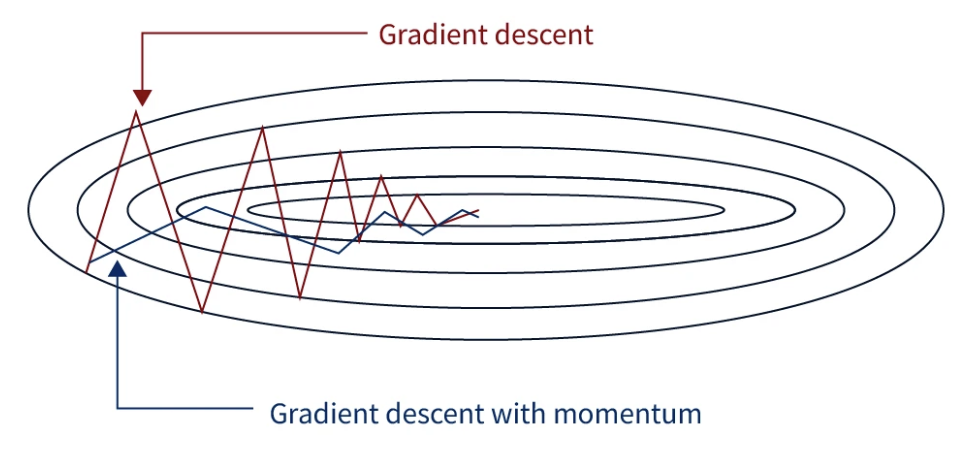
\includegraphics[scale=0.4]{figures/math/stochasticgradientdescent}
\caption{Stochastic Gradient Descent (SGD) Algorithm with and without Momentum}
\end{figure}

\begin{remark} \hlt{Nesterov Momentum}\\
Inspired by Nesterov's accelerated gradient method, the update rules are:
\begin{align}
\bm{v} &\leftarrow \alpha \bm{v} - \epsilon \nabla_{\bm{\theta}} \left(\frac{1}{m} \sum\limits_{i=1}^m L(\bm{f}(\bm{x}^{(i)}; \bm{\theta} + \alpha \bm{v}), \bm{y}^{(i)}) \right) \nonumber \\
\bm{\theta} &\leftarrow \bm{\theta} + \bm{v} \nonumber
\end{align}
Note, gradient is evaluated after current velocity is applied.\\
Hence, Nesterov momentum is adding a correction factor to the standard method of momentum.
\end{remark}

\begin{breakablealgorithm}
\caption{Stochastic Gradient Descent (SGD) with Nesterov Momentum}
\begin{algorithmic}
\Require \\
Learning rate $\epsilon_k$, Momentum parameter $\alpha$\\
Initial parameter $\bm{\theta}$, Initial velocity $\bm{v}$\\

\While {stopping criterion not met}
\State Sample a minibatch of $m$ samples from the training set $\{\bm{x}^{(1)}, \ldots, \bm{x}^{(m)} \}$ with targets $\bm{y}^{(i)}$
\State Apply interim update: $\tilde{\bm{\theta}} \leftarrow \bm{\theta} + \alpha \bm{v}$
\State Compute gradient (at interim point): $\bm{g} \leftarrow \frac{1}{m} \nabla_{\tilde{\bm{\theta}}} \sum_{i} L(f(\bm{x}^{(i)}; \tilde{\bm{\theta}}), \bm{y}^{(i)})$
\State Compute velocity update: $\bm{v} \leftarrow \alpha \bm{v} - \epsilon \bm{g}$
\State Apply update: $\bm{\theta} \leftarrow \bm{\theta} + \bm{v}$
\EndWhile
\end{algorithmic}
\end{breakablealgorithm}

\begin{figure}[H]
\centering
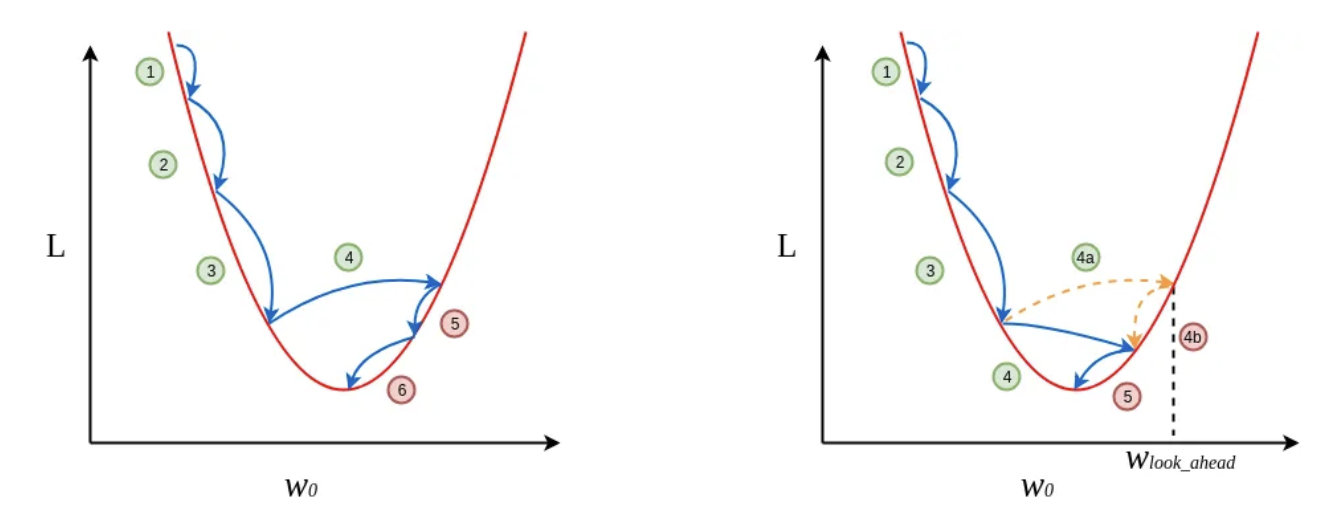
\includegraphics[scale=0.4]{figures/math/nesterov}
\caption{Momentum vs Nesterov Gradient Descent}
\end{figure}

\begin{remark} \hlt{Parameter Initialisation Challenges}\\
Training deep neural networks is difficult as most algorithms are strongly affected by choice of initialisation.\\
Designing initialisation strategies is difficult as neural network optimisation is not yet well understood, as the nice properties from initialisation may not be preserved as training proceeds.\\
Some initial points may be beneficial for optimisation, but detrimental for generalisation.
\end{remark}

\begin{remark} \hlt{Parameter Initialisation Strategies}\\
Initial parameters need to 'break symmetry' between different units. May explicitly search for large set of basis functions mutually different from each other, but this may incur noticeable computational cost.\\
Random initialisation from high-entropy distribution over high-dimensional space is computationally cheaper.\\
Larger initial weights will yield stronger symmetry breaking effect and avoid redundant units. However, if weights are set too large, may result in chaos (extreme sensitivity to small perturbations of input). Exploding gradient may be mitigated by gradient clipping. The bias (i.e., parameters encoding conditional variance of a prediction) for each unit is set to heuristically chosen constraints.
\end{remark}

\begin{remark} \hlt{Weight Initialisation Heuristics}\\
Initialising parameters of neural network $\bm{\theta}$ to $\bm{\theta}_0$ is similar to imposing a Gaussian prior $p(\bm{\theta})$ with mean $\bm{\theta}_0$, hence it make sense to choose $\bm{\theta}_0$ near $0$. Initialisation of $\bm{\theta}_0$ to large values means prior specifies which units should interact with each other, and how they should interact.\\
For a fully connected neural network with $m$ inputs and $n$ inputs, weights may be initialised by:
\begin{enumerate}[label=\roman*.]
\setlength{\itemsep}{0pt}
\item Sampling from $U\left(-\frac{1}{\sqrt{m}},  \frac{1}{\sqrt{m}} \right)$
\item Sampling from normalised initialisation $W_{i,j} \sim U \left(-\sqrt{\frac{6}{m+n}},  \sqrt{\frac{6}{m+n}} \right)$ (Glorot and Bengio). Compromise between goal of initialising all layers to have same activation variance and that of same gradient variance. Derived from assumption that network is chain of matrix multiplications with no nonlinearities.
\item Sampling from random orthogonal matrices, with scaling or gain factor $g$ that accounts for nonlinearity at each layer, with specific values for different types of nonlinear activation functions. Assumes neural network is sequence of matrix multiplications without nonlinearities. Guarantees the total number of training iterations required to reach convergence is independent of depth.\\
Increasing scaling factor $g$ pushes network toward regime where activations increase in norm in forward propagation, and gradients increase in norm in backward propagation.\\
For scaling rules that set all of initial weights to have same standard deviation, individual weight becomes extremely small when layers become large.
\item Sparse initialisation (Martens), where each unit is initialised to have exactly $k$ non-zero weight. Keep total number of input to unit independent from number of inputs $m$ without making magnitude of individual weight elements shrink with $m$.\\
Imposes very strong prior on weights that are chosen to have large Gaussian values.
\end{enumerate}
If computational resources allow, treat initial scale of weights for each layer as a hyper-parameter, and use hyper-parameter search algorithm. Choice of dense or sparse initialisation may also be a hyper-parameter.
\end{remark}

\begin{remark} \hlt{Bias Initialisation Heuristics}\\
Setting bias to zero is compatible with most weight initialisation schemes. The few other situations are:
\begin{enumerate}[label=\roman*.]
\setlength{\itemsep}{0pt}
\item If bias is for output unit, initialise bias to obtain right marginal statistics of the output. Assume initial weights are small enough that output of unit is determined only by bias. The bias will be inverse of activation function applied to marginal statistics of the output in training set.\\
If output is a highly skewed distribution over classes with marginal probability of class $i$ given by element $c_i$ of some vector $\bm{c}$, then bias vector $\bm{b}$ is such that $\text{softmax}(\bm{b}) = \bm{c}$. The models have output layers that should resemble input data $\bm{x}$, hence bias should match marginal distribution over $\bm{x}$.
\item If bias is to be set to avoid causing too much saturation at initialisation (i.e., with ReLU). Not compatible with weight initialisation schemes that do not expect strong input form bias (i.e., with random walk init).
\item If a unit controls whether other units are able to participate in a function. There is unit with output $u$ and another unit $h \in [0,1]$, multiplied together to produce output $uh$. Then $h$ is a gate that determines if $uh \approx u$ or $uh \approx 0$. Hence, to set bias for $h$ such that $h \approx 1$ at initialisation, else $u$ does not learn.
\end{enumerate}
\end{remark}

\begin{remark} \hlt{Variance or Precision Parameter Initialisation Heuristics}\\
For linear regression with conditional variance estimate using model
\begin{align}
p(y \ | \ \bm{x}) = \mathcal{N}(y \ | \ \bm{w}^T \bm{x} + b, 1/\beta) \nonumber
\end{align}
where $\beta$ is a precision parameter. The variance of precision parameters may be initialised to $1$.\\
Another approach is to assume initial weights are close enough to zero, and bias may be set while ignoring effect of the weights, then set bias to produce the correct marginal mean of the output, and set variance parameters to the marginal variance of the output in the training set.
\end{remark}

\begin{remark} \hlt{Model Parameter Initialisation with Machine Learning}\\
Initialise supervised model with parameters learned by unsupervised model trained on same inputs.\\
Alternatively, perform supervised training on a related task, which may yield initialisation that offers faster convergence than random initialisation. Information on distribution is encoded into initial parameters of model.
\end{remark}

\begin{remark} \hlt{Adaptive Gradient (AdaGrad) Algorithm}\\
Algorithm individually adapts learning rates of all model parameters by scaling them inversely proportional to square root of sum of all of their historical squared values. Has greater progress in more gently sloped directions of parameter space. On deep neural networks, accumulation of squared gradients from beginning of training can result in premature and excessive decrease in effective learning rate.
\end{remark}

\begin{breakablealgorithm}
\caption{Adaptive Gradient (AdaGrad) Algorithm}
\begin{algorithmic}
\Require \\
Global Learning rate $\epsilon$\\
Initial parameter $\bm{\theta}$\\
Small constant $\delta$, perhaps $10^{-7}$ for numerical stability\\

\State Initialise gradient accumulation variable $\bm{r} = \bm{0}$
\While {stopping criterion not met}
\State Sample a minibatch of $m$ samples from the training set $\{\bm{x}^{(1)}, \ldots, \bm{x}^{(m)} \}$ with targets $\bm{y}^{(i)}$
\State Compute gradient: $\bm{g} \leftarrow \frac{1}{m} \nabla_{\bm{\theta}} \sum_i L(f(\bm{x}^{(i)}; \bm{\theta}), \bm{y}^{(i)})$
\State Accumulate squared gradient: $\bm{r} \leftarrow \bm{r} + \bm{g} \odot \bm{g}$
\State Compute update: $\Delta \bm{\theta} \leftarrow - \frac{\epsilon}{\delta + \sqrt{\bm{r}}} \odot \bm{g}$ (Division and square root applied element-wise)
\State Apply update: $\bm{\theta} \leftarrow \bm{\theta} + \Delta \bm{\theta}$
\EndWhile
\end{algorithmic}
\end{breakablealgorithm}

\begin{remark} \hlt{Root Mean Squared Propagation (RMSProp) Algorithm}\\
Modifies AdaGrad to perform better in non-convex setting by changing gradient accumulation into exponentially weighted moving average, which discards history from extreme past so it can converge rapidly after finding a convex bowl. Use of moving average introduces a new hyper-parameter $\rho$ that controls length scale of the moving average. RMSProp is effective and practical for deep neural networks.
\end{remark}

\begin{breakablealgorithm}
\caption{Root Mean Squared Propagation (RMSProp) Algorithm}
\begin{algorithmic}
\Require \\
Global Learning rate $\epsilon$\\
Decay rate $\rho$\\
Initial parameter $\bm{\theta}$\\
Small constant $\delta$, perhaps $10^{-6}$ to stabilise division by small numbers\\

\State Initialise accumulation variable $\bm{r} = \bm{0}$
\While {stopping criterion not met}
\State Sample a minibatch of $m$ samples from the training set $\{\bm{x}^{(1)}, \ldots, \bm{x}^{(m)} \}$ with targets $\bm{y}^{(i)}$
\State Compute gradient: $\bm{g} \leftarrow \frac{1}{m} \nabla_{\bm{\theta}} \sum_i L(f(\bm{x}^{(i)}; \bm{\theta}), \bm{y}^{(i)})$
\State Accumulate squared gradient: $\bm{r} \leftarrow \rho \bm{r} + (1 - \rho) \bm{g} \odot \bm{g}$
\State Compute update: $\Delta \bm{\theta} \leftarrow - \frac{\epsilon}{\sqrt{\delta + \bm{r}}} \odot \bm{g}$ ($\frac{\epsilon}{\sqrt{\delta + \bm{r}}}$ applied element-wise)
\State Apply update: $\bm{\theta} \leftarrow \bm{\theta} + \Delta \bm{\theta}$
\EndWhile
\end{algorithmic}
\end{breakablealgorithm}

\begin{breakablealgorithm}
\caption{Root Mean Squared Propagation (RMSProp) Algorithm}
\begin{algorithmic}
\Require \\
Global Learning rate $\epsilon$\\
Decay rate $\rho$\\
Momentum coefficient $\alpha$\\
Initial parameter $\bm{\theta}$\\
Initial velocity $\bm{v}$\\

\State Initialise accumulation variable $\bm{r} = \bm{0}$
\While {stopping criterion not met}
\State Sample a minibatch of $m$ samples from the training set $\{\bm{x}^{(1)}, \ldots, \bm{x}^{(m)} \}$ with targets $\bm{y}^{(i)}$
\State Compute interim update $\tilde{\bm{\theta}} \leftarrow \bm{\theta} + \alpha \bm{v}$
\State Compute gradient: $\bm{g} \leftarrow \frac{1}{m} \nabla_{\tilde{\bm{\theta}}} \sum_i L(f(\bm{x}^{(i)}; \tilde{\bm{\theta}}), \bm{y}^{(i)})$
\State Accumulate gradient: $\bm{r} \leftarrow \rho \bm{r} + (1 - \rho) \bm{g} \odot \bm{g}$
\State Compute velocity update: $\bm{v} \leftarrow \alpha \bm{v} - \frac{\epsilon}{\sqrt{\bm{r}}} \odot \bm{g}$ ($\frac{1}{\sqrt{\bm{r}}}$ applied element-wise)
\State Apply update: $\bm{\theta} \leftarrow \bm{\theta} + \bm{v}$
\EndWhile
\end{algorithmic}
\end{breakablealgorithm}

\begin{remark} \hlt{Adaptive Moment Estimation (Adam) Algorithm}\\
Variant on combination of RMSProp and momentum. Note, momentum is incorporated directly as an estimate of first order moment of gradient; bias corrections are made to estimates of both first-order moments and second-order moments to account for initialisation at origin.\\
Algorithm is fairly robust to choice of hyper-parameters.
\end{remark}

\begin{breakablealgorithm}
\caption{Adaptive Moment Estimation (Adam) Algorithm}
\begin{algorithmic}
\Require \\
Step size $\epsilon$ (Suggested default: $0.001$)\\
Exponential decay rates for moment estimates $\rho_1, \rho_2$ in $[0,1)$ (Suggested defaults: $0.9$ and $0.999$)\\
Small constant $\delta$ used for numerical stabilisation (Suggested default: $10^{-8}$)\\
Initial parameters $\bm{\theta}$\\

\State Initialise $1$st and $2$nd momentum variables $\bm{s} = \bm{0}$, $\bm{r} = \bm{0}$
\State Initialise time step $t=0$
\While {stopping criterion not met}
\State Sample a minibatch of $m$ samples from the training set $\{\bm{x}^{(1)}, \ldots, \bm{x}^{(m)} \}$ with targets $\bm{y}^{(i)}$
\State Compute gradient: $\bm{g} \leftarrow \frac{1}{m} \nabla_{\bm{\theta}} \sum_i L(f(\bm{x}^{(i)}; \bm{\theta}), \bm{y}^{(i)})$
\State Update time step $t \leftarrow t+1$
\State Update biased first and second moment estimate: $\bm{s} \leftarrow \rho_1 \bm{s} + (1-\rho_1) \bm{g}$ and $\bm{r} \leftarrow \rho_2 \bm{r} + (1-\rho_2) \bm{g} \odot \bm{g}$
\State Correct bias in first and second moment: $\hat{\bm{s}} \leftarrow \frac{\bm{s}}{1 - \rho_1^t}$ and $\hat{\bm{r}} \leftarrow \frac{\bm{r}}{1 - \rho_2^t}$
\State Compute update: $\Delta \bm{\theta} = - \epsilon \frac{\hat{\bm{s}}}{\sqrt{\hat{\bm{r}} + \delta}}$ (Operations applied element-wise)
\State Apply update: $\bm{\theta} \leftarrow \bm{\theta} + \Delta \bm{\theta}$
\EndWhile
\end{algorithmic}
\end{breakablealgorithm}

\begin{remark} \hlt{Newton's Method}\\
Based on second-order Taylor's series approximating $J(\bm{\theta})$ near the point $\bm{\theta}_0$, ignoring higher derivatives
\begin{equation}
J(\bm{\theta}) \approx J(\bm{\theta}_0) + (\bm{\theta} - \bm{\theta}_0)^T \nabla_{\bm{\theta}} J(\bm{\theta}_0) + \frac{1}{2} (\bm{\theta} - \bm{\theta}_0)^T \bm{H}(\bm{\theta} - \bm{\theta}_0) \nonumber
\end{equation}
where $\bm{H}$ is the Hessian of $J$ with respect to $\bm{\theta}$ evaluated at $\bm{\theta}_0$.\\
Solving for critical point will get the Newton parameter update rule
\begin{equation}
\bm{\theta}^{*} = \bm{\theta}_0 - \bm{H}^{-1} \nabla_{\bm{\theta}} J(\bm{\theta}_0) \nonumber
\end{equation}
Note that for deep learning, the surface of objective function is non-convex. Regularising the Hessian will solve many of the issues such as saddle points etc.
\begin{equation}
\bm{\theta}^{*} = \bm{\theta}_0 - [H(f(\bm{\theta}_0)) + \alpha \bm{I}]^{-1} \nabla_{\bm{\theta}} J(\bm{\theta}_0) \nonumber
\end{equation}
Due to requirement for inversion of the $k \times k$ matrix with time complexity $O(k^3)$ at every training iteration, only networks with very small number of parameters may be trained with this method.
\end{remark}

\begin{breakablealgorithm}
\caption{Newton's Method with Objective $J(\bm{\theta}) = \frac{1}{m} \sum_{i=1}^m L(f(\bm{x}^{(i)}; \bm{\theta}), y^{(i)})$}
\begin{algorithmic}
\Require \\
Initial parameter $\bm{\theta}_0$\\
Training set of $m$ examples\\

\While {stopping criterion not met}
\State Compute gradient $\bm{g} \leftarrow \frac{1}{m} \nabla_{\bm{\theta}} \sum_i L(f(\bm{x}^{(i)}; \bm{\theta}), \bm{y}^{(i)})$
\State Compute Hessian: $\bm{H} \leftarrow \frac{1}{m} \nabla_{\bm{\theta}}^2 \sum_i L(f(\bm{x}^{(i)}; \bm{\theta}), \bm{y}^{(i)})$
\State Compute Hessian Inverse: $\bm{H}^{-1}$
\State Compute update: $\Delta \bm{\theta} = - \bm{H}^{-1} \bm{g}$
\State Apply update: $\bm{\theta} \leftarrow \bm{\theta} + \Delta \bm{\theta}$
\EndWhile
\end{algorithmic}
\end{breakablealgorithm}

\begin{remark} \hlt{Conjugate Gradient Method}\\
Method effectively avoids computation of inversion Hessian by descending conjugate directions, which is a search direction conjugate to the previous line search direction (will not undo progress made in that direction).\\
Let current and previous search directions be $\bm{d}_{t}, \bm{d}_{t-1}$. At training iteration $t$, the next search direction $\bm{d}_t$ is
\begin{equation}
\bm{d}_t = \nabla_{\bm{\theta}} J(\bm{\theta}) + \beta_t \bm{d}_{t-1} \nonumber
\end{equation}
note that $\beta_t$ may be computed via Fletcher Reeves:
\begin{equation}
\beta_t = \frac{\nabla_{\bm{\theta}} J(\bm{\theta}_t)^T \nabla_{\bm{\theta}} J(\bm{\theta}_t)}{\nabla_{\bm{\theta}} J(\bm{\theta}_{t-1})^T \nabla_{\bm{\theta}} J(\bm{\theta}_{t-1})} \nonumber
\end{equation}
or may be computed with Polak-Ribiere:
\begin{equation}
\beta_t = \frac{(\nabla_{\bm{\theta}} J(\bm{\theta}_t) - \nabla_{\bm{\theta}} J(\bm{\theta}_{t-1}))^T \nabla_{\bm{\theta}} J(\bm{\theta}_t)}{\nabla_{\bm{\theta}} J(\bm{\theta}_{t-1})^T \nabla_{\bm{\theta}} J(\bm{\theta}_{t-1})} \nonumber
\end{equation}
The non-linear conjugate gradient method is a variation which uses occasional resets where the method is restarted with line search along with the unaltered gradient.
\end{remark}

\begin{breakablealgorithm}
\caption{Conjugate Gradient Method}
\begin{algorithmic}
\Require \\
Initial parameter $\bm{\theta}_0$\\
Training set of $m$ examples\\
Initialise $\bm{\rho}_0 = 0$\\
Initialise $g_0 = 0$\\
Initialise $t = 1$\\

\While {stopping criterion not met}
\State Initialise the gradient $\bm{g}_t = \bm{0}$
\State Compute gradient $\bm{g} \leftarrow \frac{1}{m} \nabla_{\bm{\theta}} \sum_i L(f(\bm{x}^{(i)}; \bm{\theta}), \bm{y}^{(i)})$
\State Compute Polak-Ribiere metric: $\beta_t = \frac{(\bm{g}_t - \bm{g}_{t-1})^T \bm{g}_t}{\bm{g}_{t-1}^T \bm{g}_{t-1}}$
\State (Nonlinear conjugate gradient: optionally reset $\beta_t = 0$, i.e., if $t$ is a multiple of some constant $k$)
\State Compute search direction: $\bm{\rho}_t = -\bm{g}_t + \beta_t \bm{\rho}_{t-1}$
\State Perform line search to find: $\epsilon^{*} = \arg \min_{\epsilon} \frac{1}{m} \sum_{i=1}^m L(f(\bm{x}^{(i)}; \bm{\theta}_t + \epsilon \bm{\rho}_t), \bm{y}^{(i)})$
\State (On truly quadratic cost function, analytically solve for $\epsilon^{*}$)
\State Apply update: $\bm{\theta}_{t+1} = \bm{\theta}_{t} + \epsilon^{\theta} \bm{\rho}_t$
\State Apply time step $t \leftarrow t + 1$
\EndWhile
\end{algorithmic}
\end{breakablealgorithm}

\begin{remark} \hlt{Nonlinear Conjugate Gradients}\\
Method of conjugate gradients is still applicable for non-linear objective function.\\
Conjugate directions are no longer assumed to remain at minimum of the objective for previous directions. Has occasional resets where method of conjugate gradients is restarted with line search along unaltered gradient.
\end{remark}

\begin{remark} \hlt{Broyden-Fletcher-Goldfarb-Shanno (BGFS) Algorithm}\\
Similar to conjugate gradient, but uses more direct approach to approximation of newton's update.\\
Method approximate the inverse of hessian $\bm{H}$ with matrix $\bm{M}_t$, iteratively refined by low rank updates to better approximate $\bm{H}^{-1}$. Direction of gradient descent is then determined by $\bm{\rho}_t = \bm{M}_t \bm{g}_t$. Line search is performed in this direction to determine step size $\epsilon^{*}$. Final update of parameter is then $\bm{\theta}_{t+1} = \bm{\theta}_t + \epsilon^{*} \bm{\rho}_{t}$.\\
Note, BGFS store matrix $\bm{M}$ which requires $O(n^2)$ memory, making it impractical for most modern models.
\end{remark}

\begin{remark} \hlt{Limited Memory BFGS (L-BFGS) Algorithm}\\
Memory costs of BFGS may be decreased by not storing complete inverse Hessian approximation $\bm{M}$. L-BFGS computes approximation $\bm{M}$ with same method as BFGS, but assumes at beginning that $\bm{M}^{(t-1)}$ is the identity matrix, rather than storing the approximation between steps.\\
If used with exact line searches, directions defined by L-BFGS are mutually conjugate, and this procedure remains well-behaved when minimum of line search is reached only approximately.\\
L-BFGS may be generalised to store some vectors used to update $\bm{M}$ at each time step, costing $O(n)$ per step.
\end{remark}

\begin{remark} \hlt{Meta-Algorithm: Batch Normalisation}\\
An update from optimisation algorithm may result in multiple-order effects, and in very deep networks, even higher-order interactions can be significant.\\
Batch normalisation provides an elegant way of re-parametrising any deep network, which reduces the problem of coordinating updates across multiple layers. Batch normalisation may be applied to any input/hidden layer.\\
Let $\bm{H}$ be minibatch of activations of layer to normalise, with activations for each example appearing in a row. To normalise $\bm{H}$, replace it with $\bm{H}' = \frac{\bm{H} - \bm{\mu}}{\bm{\sigma}}$ where $\bm{\mu}$ is a vector of mean of each unit and $\sigma$ is a vector of standard deviation of each unit. Then $H_{ij}$ is normalised by subtracting $\mu_j$ and dividing $\sigma_j$. Rest of network then operates on $\bm{H}'$ just as in original network on $\bm{H}$.\\
At training, the mean and standard deviations are computed as
\begin{align}
\bm{\mu} &= \frac{1}{m} \sum\limits_i \bm{H}_{i, ;}, \ \ \ \bm{\sigma} = \sqrt{\delta + \frac{1}{m} \sum\limits_{i} (\bm{H} - \bm{\mu})^2_i} \nonumber
\end{align}
where $\delta$ is a small positive value (i.e., $10^{-8}$) to avoid undefined gradient of $\sqrt{z}$ at $z=0$.\\
These are then back-propagated to normalise $\bm{H}$, hence gradient will never increase the standard deviation or mean of $h_i$. Batch normalisation re-parametrises the model to make some units always standardised.\\
At test time, $\mu$ and $\sigma$ may be replaced by running averages from training time. This allows model to be evaluated on a single example, without needing to use definitions of $\mu$ and $\bm{\sigma}$ that depends on entire minibatch.
\end{remark}

\begin{remark} \hlt{Batch Normalisation but Maintain Network Express Power}\\
Replace batch of hidden activations $\bm{H}$ with $\bm{\gamma} \bm{H}' + \bm{\beta}$ rather than $\bm{H}'$, where $\bm{\gamma}$ and $\bm{\beta}$ are learned parameters to allow new variable to have any mean and standard deviation. With original $\bm{H}'$, mean of $\bm{H}$ was determined by complicated interaction between parameters in layers below $\bm{H}$. With $\bm{\gamma} \bm{H}' + \bm{\beta}$, the mean is determined solely by $\bm{\beta}$, which is much easier to learn with gradient descent.\\
Most neural network layers are of form $\phi(\bm{X} \bm{W} + \bm{b})$, where $\phi$ is some fixed nonlinear activation function. Then $\bm{X} \bm{W} + \bm{b})$ should be replaced by normalised version of $\bm{X} \bm{W}$, and bias term omitted as it becomes redundant with $\beta$ parameter applied from batch normalisation re-parametrisation. Statistics of input are non-Gaussian and less amenable to standardisation by linear operations.
\end{remark}

\begin{remark} \hlt{Meta-Algorithm: Coordinate Descent}\\
	
\end{remark}







    % Microstructure Trading Section
    \newpage
    %\section{Market Microstructure}


\subsection{Market Fundamentals}

The basic function of a market is to bring buyers and sellers together.

\begin{process}
\hlt{(Four Components of a Trade)}
\begin{enumerate}[label=\roman*.]
\setlength{\itemsep}{0pt}
\item Acquisition of information and quotes
\begin{enumerate}[label=\arabic*.]
\setlength{\itemsep}{0pt}
\item Quality information and transparency are crucial to price discovery
\item Transparent markets quickly disseminate high-quality information
\item Opaque markets are those that lack transparency
\end{enumerate}
\item Routing of the trade order
\begin{enumerate}[label=\arabic*.]
\setlength{\itemsep}{0pt}
\item Selecting the brokers to handle the trades
\item Deciding which markets will execute the trades and transmitting the trades to the markets
\end{enumerate}
\item Execution. Buys are matched and executed against sells according to the rules of the market
\item Confirmation, clearance and settlement
\begin{enumerate}[label=\arabic*.]
\setlength{\itemsep}{0pt}
\item Clearance is the recording and comparison of the trade records
\item Settlement involves the actual delivery of the security and its payment
\item Might include trade allocation
\end{enumerate}
\end{enumerate}
\end{process}

\begin{remark}
\hlt{(Risks of Algorithmic Trading)}
\begin{enumerate}[label=\roman*.]
\setlength{\itemsep}{0pt}
\item Leaks might arise from competitor efforts to revere engineer them
\item Many algorithms lack the capacity to handle or respond to exceptional or rare events.
\end{enumerate}
\end{remark}

\begin{remark}
\hlt{(Cornering-the-Market)} Trader takes huge long futures position and tries to exercise control over supply of underlying commodity. As maturity of futures contract is approaching, position is not closed, number of outstanding contracts exceed commodities available. Holders of short positions desperately try to close positions, leading to rise in both futures and spot prices.\\
Abuse is dealt with by increasing margin requirements or imposing stricter position limits or prohibiting trades that increase speculator's open position or requiring market participants to close their positions.
\end{remark}

\subsubsection{Liquidity Access in Equity Markets}

\hlt{(Exchanges)} Account for $60\%$ to $70\%$ of all activity. The full order-book, arrivals/cancellations are all published, the liquidity information is transparent. Larger orders may impact the market. Liquidity at best price cannot be ignored, as the exchange will need to reroute to other exchanges where price is better while charging a fee (National Best Bid Offer, NBBO). All exchanges have almost exactly the same trading mechanism, and behave exactly the same way during the trading day except for opening and closing auctions.\\
Most exchanges use maker-taker fee model, but some exchanges (BYX, EDGA, NSX, BX) have an inverted fee model where rebate is provided for taking liquidity. IEX uses a speed bump to remove speed advantages of HFTs, providing a less 'toxic' liquidity pool.\\

\hlt{(Dark Pools/ATS)} Dark pools do not display any order information and use the NBBO as reference price. To avoid accessing protected venues, these pools trade only at the inside market (at or within the bid ask spread). Still possible to identify large blocks of liquidity by 'pinging' the pool at minimum lot size; counteracted by sending orders with minimum fill quantity tag, which allows block to be transparent from small pinging.\\
Most of ATS are run by major investment banks; some venues allow direct trading between investment firms. Note that many of the trading strategies used by firms tend to be highly correlated, hence liquidity is often on the same side; venues have to leverage sell side broker's liquidity to supplement their own.\\

\hlt{(Single Dealer's Platform/Systematic Internalisers)} Broker/Dealer and other institutional clients connect to Single Dealer Platform (SDP) directly. Not regulated ATS, hence can offer unique products. Brokers provide their own SDPs to expose their internal liquidity.\\

\hlt{(Auctions)} Exchanges begin and end day with a primary auction procedure that leverages special order types to accumulate supply and demand, then run algorithm that determines best price that would at best pair off the most volume. An opportunity for active and passive investors to exchange large amounts of liquidity.

\subsubsection{Trading Mechanisms}

Most common approach by modern electronic exchanges is the time/price priority, \hlt{continuous double auction} trading system. There are multiple buyers and multiple sellers participating at the same time.\\

\hlt{(Limit Order Book, LOB)} Stores all non-executed orders with associated instructions. Highly efficient, able to handle a high degree of concurrency to ensure the state is always correct. Has 2 copies of core data structure (for Buy, Sell orders). Supports 3 basic instruction types (insert, cancel, amend). There are 4 events on both Buy and Sell that may alter state of order book (limit order submission, limit order cancellation, limit order amendment, execution).\\

\hlt{(Matching Algorithm)} Responsible for interpreting various events to determine if any buy and sell orders can be matched. When multiple orders can be paired, price/time priority is used, where the order with most competitive prices are matched, and when prices are equal, the order that arrived prior is chosen.\\

Exchanges will publish order imbalance that exists among orders on opening and closing books during \hlt{Open Auctions}, with indicative price and volume. The following are published every second on market data feeds:
\begin{enumerate}[label=\roman*.]
\setlength{\itemsep}{0pt}
\item \hlt{Current Reference Price}: Price at which paired shares are maximised, imbalance is minimised, distance from bid-ask mid-point is minimised, in that order
\item \hlt{Near Indicative Clearing Price}: The crossing price at which orders in opening, closing book and continuous book would clear against each other
\item \hlt{Far Indicative Clearing Price}: The crossing price at which orders in opening, closing book would clear against each other
\item \hlt{Number of Paired Shares}: The number of on-open or on-close shares that is able to pair off at the current reference price
\item \hlt{Imbalance Shares}: The number of opening or closing shares that would remain unexecuted at the current reference price
\item \hlt{Imbalance Side}: The side of imbalance. B is buy-side imbalance; S is sell-side imbalance; N is no imbalance; O is no marketable on-open or on-close orders
\end{enumerate}

In general, the following rules apply to match supply and demand:
\begin{enumerate}[label=\roman*.]
\setlength{\itemsep}{0pt}
\item Crossing price must maximise volume transacted
\item If several prices result in similar volume transacted, the crossing price is the one the closest from last price
\item Cross price is identical for all orders executed
\item If two orders are submitted at same price, the order submitted first has priority
\item It is possible for an order to be partially executed if the other side quantity is not sufficient
\item 'At Market' orders are executed against each other at the determined crossing price, up to available matching quantity on both sides, but generally do not participate in price formation process
\item For Open Auction, unmatched 'At Market' orders are entered into continuous session of LOB as limit orders at the crossing price
\end{enumerate}

The open auction is a major price discovery mechanism, as it occurs after a period of market inactivity when market participants were unable to transact even if they have information. Market participants with better information are more likely to participate, with more aggressive orders to extract liquidity, hence the mechanism is quite volatile and more suited for short-term alpha investors.\\
During execution, smaller orders may avoid participation in open auction and period thereafter; larger orders may participate to extract significant liquidity from the market.\\

Diversity of order types is key component of continuous double auction electronic markets.

\begin{definition} {\color{white}space}
\begin{enumerate}[label=\roman*.]
\setlength{\itemsep}{0pt}
\item \hlt{Market Order}: trade carried out immediately at best price available in market.
\item \hlt{Limit Order}: only executed at this price or at one more favourable to the trader.
\item \hlt{Stop/Stop-Loss Order}: not visible in LOB. Only become active when certain price is reached or passed, then enter order book as ether limit or market order depending on user setup.
\item \hlt{Stop-Limit Order}: combination of stop order and limit order. Order becomes limit order as soon as a bid or ask is made at the price equal to or less favourable than stop price. If stop price and limit price is the same, then the order is \hlt{stop-and-limit} order.
\item \hlt{Trailing Stop Order}: function like stop orders, but stop price is set dynamic rather than static.
\item \hlt{Market-if-Touched (MIT)/Board Order}: executed at best available price after trade occurs at a specified price or more favourable. Ensure profit is taken if sufficiently favourable price movements occur.
\item \hlt{Market-Not-Held/Discretionary Order}: traded as market order, execution may be delayed at broker's discretion for better price.
\item \hlt{All-Or-None Order}: request full execution of order. Not executed until full quantity is available.
\item \hlt{Peg Order}: specify a price level at which order should be continuously and automatically repriced. Used for mid-point executions in non-displayed markets.
\item \hlt{Iceberg Order}: limit order with specific display quantity, designed to prevent information leakage.
\item \hlt{Hidden Order}: when available to trade, not directly available to other market participants in central LOB
\item \hlt{On-Open}: request execution at open price. Can be limit-on-open or market-on-open.
\item \hlt{On-Close}: request execution at close price. Can be limit-on-close or market-on-close.
\item \hlt{Imbalance Only}: provide liquidity intended to offset on-open/on-close order imbalances during opening/closing cross. These generally are limit orders.
\item \hlt{D-Quote}: Special order on NYSE, mainly used during close auction period.
\item \hlt{Funari}: Special order on Tokyo Stock Exchange, allows limit order placed in book during continuous session to automatically enter closing auction as market orders.
\end{enumerate}
\end{definition}

Instruction validity may take the following forms:
\begin{enumerate}[label=\roman*.]
\setlength{\itemsep}{0pt}
\item \hlt{Day Order}: valid for full duration of trading session
\item \hlt{Extended Day Orders}: allows for trading in extended hours
\item \hlt{Good-Till-Cancel Order}: in effect until executed or until end of trading in particular contract
\item \hlt{Immediate-or-Cancel Order}: will be immediately cancelled back to sender after reaching matching engine if it does not get immediate fill.
\item \hlt{Fill-or-Kill Order}: must be executed immediately on receipt or none at all.
\end{enumerate}


\subsubsection{Market Microstructure Primer}

A market microstructure analysis framework follows three main categories:
\begin{enumerate}[label=\roman*.]
\setlength{\itemsep}{0pt}
\item Price Formation and Price Discover: how prices impound information over time, and how determinants of trading costs vary
\item Market Design: impact of trading rules on price formation. Choice of tick size, circuit breakers that halt trading in event of large price swings, degree of anonymity, transparency of information to market participants. These create a diverse set of constraints and opportunities.
\item Transparency: quantity, quality and speed of information effect on trading process. Classified into pre-trade (lit order book), post-trade (trade reporting to public). 
\end{enumerate}

Topics for research in microstructure includes the following:
\begin{enumerate}[label=\roman*.]
\setlength{\itemsep}{0pt}
\item Parent order sliced into several child orders sent to market for execution; difficult to discern the informed trader who use sophisticated dynamic algorithms. Retail trades usually cross the spread.
\item Understanding of trading intensity in short intervals. Order imbalance is empirically shown to be unrelated to price levels.
\item Informed traders usage of hidden orders in entering and exiting the market require further studies.
\item Traders respond to changing market conditions by revising quoted prices. Quote volatility can provide valuable information about perceived uncertainty in the market.
\end{enumerate}


    % Equities Trading Section
    \newpage
    %\section{Equities Trading}



    % Fixed Income Trading Section
    \newpage
    %\section{Fixed Income Trading}



    % Derivatives Trading Section
    \newpage
    %\section{Derivatives Trading}

Based on the classic by John C. \cite{hull_2021}

\subsection{Fundamentals of the Market}

The derivatives market is much larger than the stock market in terms of underlying assets. Derivatives may be used for hedging, speculation, or arbitrage; and also transfer a wide range of risks from one entity to another.

\begin{definition} A \hlt{derivative} involves two parties agreeing to a future transaction, with value depending on the values of other underlying variables.
\end{definition}

A derivatives exchange is a market where individuals and companies trade standardised contracts as defined by the exchange. Once two traders have agreed to trade a product offered by the exchange, it is handled by the exchange clearing house, which takes care of the credit risk by requiring each trade to deposit margin.\\

If the trade is taken over-the-counter (OTC), participants may present it to a central counterparty (CCP) or clear the trade bilaterally. With the 2008 financial crisis, OTC market is forced to become more like the exchange-traded market, with changes as follows:
\begin{enumerate}[label=\roman*.]
\setlength{\itemsep}{0pt}
\item Standardised OTC derivatives between two financial institutions in US must, whenever possible, be traded on a swap execution facility (SEF), where market participants can post bid and ask quotes, and can trade by accepting the quotes of other market participants.
\item Require that a CCP be used for most standardised derivatives transactions between financial institutions.
\item All trades must be reported to a central repository.
\end{enumerate}

\subsubsection{Forward, Futures, and Options}

\begin{definition} A \hlt{spot contract} is an agreement to buy or sell an asset almost immediately. A \hlt{forward contract} is an agreement or buy or sell an asset at a certain future time for a certain price.
\end{definition}

Let $S_T$ be the spot price of asset at maturity, $K$ is delivery price.\\
The payoff from a long position in a forward contract is $S_T - K$.\\
The payoff from a short position in a forward contract is $K - S_T$.\\

Futures contract are traded on an exchange, unlike forwards which are traded OTC. Majority of futures contract do not lead to delivery, as positions are closed prior to delivery period by entering an opposite trade to the original one.\\

Party in short position may file notice of intention to deliver with the exchange when they are ready to deliver. If the asset is a commodity, the grade of commodity are specified. The contract size specifies the amount of asset that has to be delivered. The place for delivery must also be specified, as commodities may involve significant transportation costs. The delivery month of the commodity may also be specified, and are chosen by the exchange to meet the needs of market participants. Trading typically ceases a few days before the last day on which delivery can be made. Daily price movement limits are also specified by exchange to prevent speculative excess causing large price movements; in this case trading ceases for the day.\\

As the delivery price for a futures contract is approached, the futures price converges to the spot price of the underlying asset.
\begin{figure}[H]
\centering
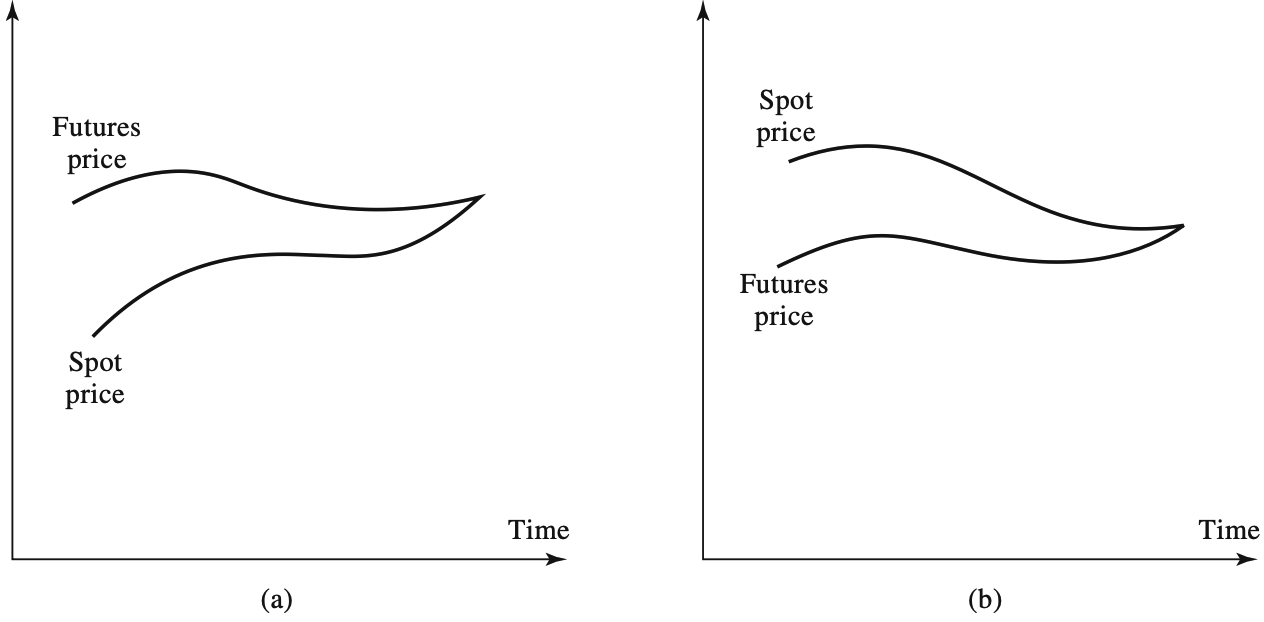
\includegraphics[scale=0.4]{derivatives/convgspotfuture}
\caption{Convergence of futures price to spot price.}
\end{figure}

Suppose futures price is above spot price during delivery period. Traders have clear arbitrage opportunity: short futures, long asset, make delivery. The futures price will then fall.\\
If futures price is below spot price during delivery period, traders will long futures, wait for delivery, and the futures price will then rise.\\

Options are traded both on exchanges and OTC.

\begin{definition} A \hlt{call option} (\hlt{put option}) gives the holder the right to sell (buy) the underlying asset by a certain date for a certain price.
\end{definition}

\begin{definition} An \hlt{American option} can be exercised at any time up to expiration date. An \hlt{European option} can only be exercised on expiration date itself.
\end{definition}

\subsubsection{Clearing House}

Margin accounts are used by exchanges to organise trading so that contract defaults are avoided. \\
Trader has to keep funds in a margin account; the amount to be deposited at the time the contract is entered into is the \hlt{initial margin}. At each of trading day, margin account is adjusted to reflect trader's P\&L (\hlt{daily settlement}, \hlt{marking to market}). Daily settlement leads to funds flowing daily between traders with long positions and traders with short positions; this daily flow of funds to reflect P\&L is the \hlt{variation margin}. Trading via brokers requires a \hlt{maintenance margin}, which is lower than initial margin; if balance in margin account falls below maintenance margin, trader receives \hlt{margin call} and is required to top up to initial margin level within short period of time, or else broker closes out the position. Trader is also entitled to withdraw any balance in margin account that is in excess of the initial margin. Brokers pay interest on balance in margin account.\\
A forward contract is settled at end of life, while futures contract is settled daily. Minimum levels for initial and maintenance margins are set by exchange clearing house. Minimum margin levels are determined by variability of the price of underlying asset, revised when necessary.\\

The clearing house acts as intermediary in futures transactions, and keep track of all daily transactions for calculating net positions of each of its members. Members must provide initial margin reflecting the total number of contracts cleared. The maintenance margin is set equal to initial margin. In determining margin requirements, the number of contracts outstanding is calculated on a net basis rather than a gross basis. Members are required to contribute to a guaranty fund, which is used in the event that a member defaults, and the member's margin is insufficient to cover losses.

\subsubsection{OTC Markets}

OTC markets use central counterparties (CCPs), which perform the same role as exchange clearing houses. Members of CCP provide both initial margin and daily variation margin, and contribute to a guaranty fund. If an OTC derivative transaction has been agreed upon between parties A and B, and CCP accepts the transaction, they become the counterparty to both A and B. CCP hence takes on credit risk of both A and B.\\
Transactions are valued daily, and there are daily variation margin payments between members.\\

For bilaterally cleared OTC, two companies enter a master agreement covering all their trades (ISDA). The agreement includes a credit support annex (CSA), requiring both parties to provide collateral. Collateral agreements in CSAs usually require transactions to be valued daily. Since 2016, regulations require both initial margin and variation margin between financial institutions.

{

\begin{definition} \hlt{Credit spread} is the difference between the interest rate and risk free rate.
\end{definition}

\hlt{(Treasury Rates)} The rates on Treasury bills and Treasury bonds. The Treasury rates of developed countries are regarded as risk-free rates, as it is assumed that there is no chance the government will default.\\

\hlt{(Overnight Rates)} Borrowing and lending overnight by financial institutions to match asset and liabilities requirements for reserves; the overnight rate is the \hlt{federal funds rate}. The weighted average of rates in brokered transactions is the \hlt{effective federal funds rate}. The Federal Reserve may intervene with its own transactions to raise or lower the rates.\\

\hlt{(Repo Rates)} Secured borrowing rates; the difference between the price at which securities are sold and then repurchased. If structured carefully, involves very little credit risk. Most common type of repo is an \hlt{overnight repo}. In longer term arrangements, \hlt{term repos} are used.\\

The terminal value of an investment $A$ invested at interest rate of $R$ per annum, compounded $m$ times per annum, is $A(1+\frac{R}{m})^{mn}$. If $m=1$, the rate is the \hlt{equivalent annual interest rate}. If continuous compounded is used, then  the terminal value at the end of a year is $Ae^{R}$.\\

The \hlt{$n$-year spot-rate} is the interest rate earned on a zero-coupon bond. The \hlt{Bond Price} is the present value of all cash flows that will be received by owner of the bond, with different spot rate for each cash flow. The \hlt{Bond Yield} is the discount rate that, when applied to all cash flows, gives a bond price equal to its market price. The \hlt{Par Yield} for a certain bond maturity is the coupon rate that causes the bond price to equal its par value.\\

\begin{definition}
\hlt{Forward Rates} are rates implied by current spot rates for periods of time in the future.
\end{definition}

Given $R_1, R_2$ the spot rates for maturities $T_1, T_2$ respectively, and $R_F$ the forward rate between $T_1$ and $T_2$, then
\begin{equation}
R_F = \frac{R_2 T_2 - R_1 T_1}{T_2 - T_1}=R_2 + (R_2 - R_1)\frac{T_1}{T_2 - T_1} \nonumber
\end{equation}
Given the spot rate $R$ for maturity $T$, the \hlt{instantaneous forward rate} for maturity of $T$ is then
\begin{equation}
R_F = R + T \frac{\partial R}{\partial T} \nonumber
\end{equation}
If $P(0,T) = e^{-RT}$ is the price of zero-coupon bond maturity at time $T$, the equation is then
\begin{equation}
R_F = -\frac{\partial}{\partial T} \ln P(0,T) \nonumber
\end{equation}

\begin{definition}
\hlt{Forward Rate Agreement (FRA)} is an agreement to exchange a predetermined rate for a reference rate that will be observed in the market at a future time.
\end{definition}

Let $R_K$ be the fixed rate, $R_F$ be the current forward rate for the reference rate, $\tau$ be the period of time to which the rates apply, $L$ be the principal in the contract.\\
For the party that receives the fix rate, the FRA has a present value of 
\begin{equation}
\tau (R_K - R_F)L \nonumber
\end{equation}
For the party that pays the fix rate, the FRA has a present value of
\begin{equation}
\tau (R_F - R_K)L \nonumber
\end{equation}

\begin{definition}
The \hlt{Duration} of a bond is a measure of how long the holder of the bond has to wait before receiving the present value of the cash payments.
\end{definition}

Let $c_i$ be cash flow at time $t_i$ ($1 \leq i \leq n$). Bond price $B$, yield $y$ (continuously compounded) are related by
\begin{equation}
B = \sum\limits_{i=1}^n c_i e^{-y t_i} \nonumber
\end{equation}
The Duration $D$ of the bond is then
\begin{equation}
D = \sum\limits_{i=1}^n t_i \left[ \frac{c_i e^{-y t_i}}{B} \right] \nonumber
\end{equation}
where the term in square brackets is ratio of present value of cash flow at $t_i$ to bond price. Duration is hence a time-weighted average of the times when payments are made.\\
The relationship between duration and yield is as follows:
\begin{align}
\Delta B &= \frac{dB}{dy} \Delta y \nonumber \\
\frac{\Delta B}{B} &= - D \Delta y \nonumber
\end{align}

If $y$ is expressed with compounding frequency of $m$ times a year, then the relationship becomes
\begin{equation}
\Delta B = - \frac{BD \Delta y}{1 + y/m} \nonumber
\end{equation}
Hence, the \hlt{modified duration} is 
\begin{equation}
D^* = \frac{D}{1 + y/m} \nonumber
\end{equation}
The duration relationship is then
\begin{equation}
\Delta B = - B D^* \Delta y \nonumber
\end{equation}

When duration is used for bond portfolios, it is assumed that the yields of all bonds will change by approximately the same amount, i.e., a parallel shift in the spot yield curve. The portfolio may still be exposed to shifts that are either large or non-parallel.\\
\hlt{Convexity} may be used to improve the relationship in the equation. Convexity is defined as
\begin{equation}
C = \frac{1}{B} \frac{d^2 B}{dy^2} \nonumber
\end{equation}
By Taylor series, we then have the relationship
\begin{equation}
\frac{\Delta B}{B} = -D \Delta y + \frac{1}{2}C(\Delta y)^2 \nonumber
\end{equation}

To determine the underlying reasons for the shape of the spot curve, theories on term structure of interest rates are referred to.\\

\hlt{(Expectations Theory)} A forward interest rate corresponding to a certain future period is equal to the expected future zero interest rate for that period.\\

\hlt{(Market Segmentation Theory)} There exists no relationship between short, medium, and long-term interest rates, as investors do not readily switch from one maturity to another.\\

\hlt{(Liquidity Preference Theory)} Investors prefer to preserve their liquidity and invest funds for short periods of time. Borrowers prefer to borrow at fixed rates for long periods of time. Hence forward rates are greater than expected future spot rates.






\newpage

\subsection{Forwards and Futures}

Based on the book by John \cite{hull_2021}.

\subsubsection{Pricing}

To examine how forward prices and futures prices are related to spot price, we assume the following are true for some market participants:
\begin{enumerate}[label=\roman*.]
\setlength{\itemsep}{0pt}
\item No transaction costs
\item Same tax rate on all net trading profits
\item Money borrowed and lend are at the same risk-free rate
\item Arbitrage opportunities are taken advantaged of as they occur
\end{enumerate}

Let $T$ be time until delivery date (in years), $S_0$ be price of underlying asset today, $F_0$ be price of forward or futures today, $r$ be zero-coupon risk-free rate per annum in continuous compounding (maturing in $T$ years).\\

Consider a forward contract on underlying asset with spot price $S_0$ that provides no income. Then
\begin{equation}
F_0 = S_0 e^{rT} \nonumber
\end{equation}
If $F_0 > S_0 e^{rT}$, long asset and short forward. If $F_0 < S_0 e^{rT}$, short asset and long forward.\\
If short sales are not possible, and arbitrage opportunities exist, then if $F_0 > S_0 e^{rT}$, investor may:
\begin{enumerate}[label=\arabic*.]
\setlength{\itemsep}{0pt}
\item Borrow $S_0$ in cash at an interest rate $r$ for $T$ years
\item Buy 1 unit of asset
\item Enter forward contract to sell $1$ unit of asset
\end{enumerate}
At time $T$, asset is sold for $F_0$, investor to repay $S_0 e^{rT}$ loan, making profit $F_0 - S_0 e^{rT}$.\\
If $F_0 < S_0 e^{rT}$, investor may:
\begin{enumerate}[label=\arabic*.]
\setlength{\itemsep}{0pt}
\item Sell asset for $S_0$
\item Invest proceeds at interest rate $r$ for time $T$
\item Enter into forward contract to buy $1$ unit of asset
\end{enumerate}
At time $T$, cash has grown to $S_0 e^{rT}$. Investor repurchase asset for $F_0$, makes profit of $S_0 e^{rT} - F_0$.\\

If the underlying asset provide income with present value of $I$ during life of forward, then
\begin{equation}
F_0 = (S_0 - I)e^{rT} \nonumber
\end{equation}
If $F_0 > (S_0 - I)e^{rT}$, investor may long asset and short forward. If $F_0 < (S_0 - I)e^{rT}$, investor may short asset and long forward. If short sales are not possible, investors owning the asset will sell the asset and long forward.\\

If the underlying asset provides a known yield rather than income, with $q$ as the average yield, then the following strategy must generate zero profit to prevent arbitrage:
\begin{enumerate}[label=\arabic*.]
\setlength{\itemsep}{0pt}
\item Borrow $S_0$ to buy one unit of asset at time $0$
\item Enter into forward to sell $e^{qT}$ units of asset at time $T$ for $F_0$
\item Close the forward by selling $e^{qT}$ units of the asset at time $T$
\end{enumerate}
Hence we have
\begin{equation}
S_0 e^{rT} = e^{qT} F_0 \nonumber 
\end{equation}
or
\begin{equation}
F_0 = S_0 e^{(r-q)T} \nonumber
\end{equation}

When a forward contract is first entered, the value is close to zero. Let $K$ be delivery price negotiated some time ago, with $T$ years delivery date, $r$ is $T$-year risk-free interest rate, $F_0$ is forward price if contract is negotiated today. Let $f$ be value of forward contract today. Then
\begin{equation}
f = (F_0 - K)e^{-rT} \nonumber
\end{equation}

In the case of stock indices, if $F_0 > S_0 e^{(r-q)T}$, profit can be made by buying stocks underlying the index at spot price and shorting the index futures contract. If $F_0 < S_0 e^{(r-q)T}$, short the stocks and long futures. This is known as \hlt{index arbitrage}.\\

In the case of currencies, let $r_f$ be foreign risk-free rate in a foreign-denominated bond, $S_0$ be spot price of local currency in foreign currency, $F_0$ be forward or future price of local currency in foreign currency. Then the \hlt{interest rate parity} relation persists in the form
\begin{equation}
F_0 = S_0 e^{(r-r_f)T} \nonumber
\end{equation}

For commodities, let $U$ be present value of storage costs net of income during life of forward. Then
\begin{equation}
F_0 = (S_0 + U)e^{rT} \nonumber
\end{equation}
If storage costs are proportional to price of commodity, they can be treated as negative yield. Let $u$ be storage costs per annum as proportion of spot price net of any yield earned on asset. Then
\begin{equation}
F_0 = S_0 e^{(r+u)T} \nonumber
\end{equation}
If $F_0 > (S_0 + U)e^{rT}$, then investor may take advantage of arbitrage:
\begin{enumerate}[label=\arabic*.]
\setlength{\itemsep}{0pt}
\item Borrow $S_0 + U$ at risk-free rate, purchase one unit of commodity and pay storage costs
\item Short futures on one unit of commodity
\end{enumerate}
If $F_0 < (S_0 + U)e^{rT}$, then investor may take advantage of arbitrage:
\begin{enumerate}[label=\arabic*.]
\setlength{\itemsep}{0pt}
\item Sell commodity, save storage costs, invest proceeds at risk-free interest rate
\item Long futures contract
\end{enumerate}

Benefits from holding physical assets are \hlt{convenience yields}, such as by crude oil manufacturers. Let $y$ be the convenience yield, then
\begin{equation}
F_0 e^{yT} = (S_0 + U)e^{rT} \nonumber
\end{equation}
If storage costs per unit are a constant proportion of spot price, then $y$ is defined such that
\begin{equation}
F_0 e^{yT} = S_0 e^{(r+u)T} \nonumber
\end{equation}
Convenience yield reflects market expectation on future availability of the commodity. The greater the possibility that shortages will occur, the higher the commodity yield.

The \hlt{cost of carry} measures storage cost plus interest paid to finance the asset less income earned:
\begin{enumerate}[label=\roman*.]
\setlength{\itemsep}{0pt}
\item Non-dividend paying stock: $r$, as no storage and income is earned
\item Stock index: $r-q$, as income is earned at rate $q$ on asset
\item Currency: $r - r_f$
\item Commodity: $r-q+u$, where it provides income at rate $q$ and requires storage costs at rate $u$
\end{enumerate}

\subsubsection{Hedging with Futures}

The fundamentals of hedging with futures are \hlt{hedge-and-forget} strategies, where no changes is made to adjust the hedge once it has been put in place.

\begin{definition}
\hlt{(Basic Principles of Futures Hedging)}\\
The objective is to take a position that neutralises the risk as far as possible.
\begin{enumerate}[label=\roman*.]
\setlength{\itemsep}{0pt}
\item \hlt{Short Hedge}: short position on futures. \\
Used when hedger already owns an asset and will sell the asset at some time in the future; or when asset is not owned right now but will be owned and ready for sale sometime in the future.
\item \hlt{Long Hedge}: long position on futures. \\
Used when hedger will purchase an asset in the future and wants to lock in the price now.
\end{enumerate}
\begin{table}[h]
\begin{tabular}{|c | c | c|}
\hline
 & \textbf{Short Hedge} & \textbf{Long Hedge} \\ \hline
May $15$ & \makecell[l]{Spot: $50$ \\ Futures: $49$} & \makecell[l]{Spot: $50$ \\ Futures: $49$} \\ \hline
August $15$ Scenario 1 & \makecell[l]{Spot: $45$ \\ Gain from hedge: $4$} &  \makecell[l]{Spot: $45$ \\ Loss from hedge: $4$} \\ \hline
August $15$ Scenario 2 & \makecell[l]{Spot: $55$ \\ Loss from hedge: $6$} & \makecell[l]{Spot: $55$ \\ Gain from hedge: $6$} \\ \hline
\end{tabular}
\end{table}
\end{definition}

In practice, hedging is not perfect due to factors as follows:
\begin{enumerate}[label=\arabic*.]
\setlength{\itemsep}{0pt}
\item Asset being hedged is not exactly the same as the asset underlying the futures contract.
\item Uncertainty as to exact date in which the asset will be bought or sold.
\item Hedge may require the futures contract to be closed out before its delivery month.
\end{enumerate}
These lead to \hlt{basis risk}.

\begin{definition}
The \hlt{basis} in a hedging situation is defined as
\begin{align}
\text{Basis} = \text{Spot Price} - \text{Futures Price} \nonumber
\end{align}
An increase/decrease in basis is a strengthening/weakening of the basis.
\end{definition}

\begin{definition}
Let $S_i$ be spot price at time $t_i$, $F_i$ be futures price at time $t_i$, $b_i$ be basis price at time $t_i$.	 Assume hedge is placed at time $t_1$, closed at time $t_2$. Price realised for asset is $S_2$, profit from futures position is $F_1 - F_2$.  Effective price obtained for asset hedging is therefore $S_2 + F_1 - F_2 = F_1 + b_2$.\\
If $b_2$ is known, perfect hedge will result. The \hlt{basis risk} is the hedging risk from uncertainty associated with $b_2$.
\end{definition}

\begin{definition}
\hlt{Cross Hedging} occurs when the asset underlying the futures contract is not the same as the asset whose price is being hedged.
\end{definition}

Cross hedging is often used when futures of the original asset being hedged are not actively traded on the market, and the hedger seeks an alternative asset to hedge the original asset.

\begin{definition}
\hlt{Hedge Ratio} is the ratio of size of position taken in futures contract to the size of exposure.
\end{definition}

Assuming no daily settlement of futures contracts, hedger seeks a hedge ratio that minimises variance of hedged position value. Let $\Delta S$ be change in spot price, $\Delta F$ change in futures price. Assuming linear relationship,
\begin{equation}
\Delta S = a + b \Delta F + \epsilon	 \nonumber
\end{equation}
where $a,b$ are constants, $\epsilon$ is an error term. Suppose hedge ratio is $h$. Change in value of position per unit of exposure to $S$ is:
\begin{equation}
\Delta S - h \Delta F = a + (b-h) \Delta F + \epsilon \nonumber
\end{equation}
Standard deviation is minimised by setting $h=b$. Let minimum variance hedge ratio be $h^*$. Then
\begin{equation}
h^* = \rho \frac{\sigma_S}{\sigma_F} \nonumber
\end{equation}
where $\sigma_S, \sigma_F$ is standard deviation of $\Delta S, \Delta F$ respectively, $\rho$ is coefficient of correlation.

\begin{figure}[H]
\centering
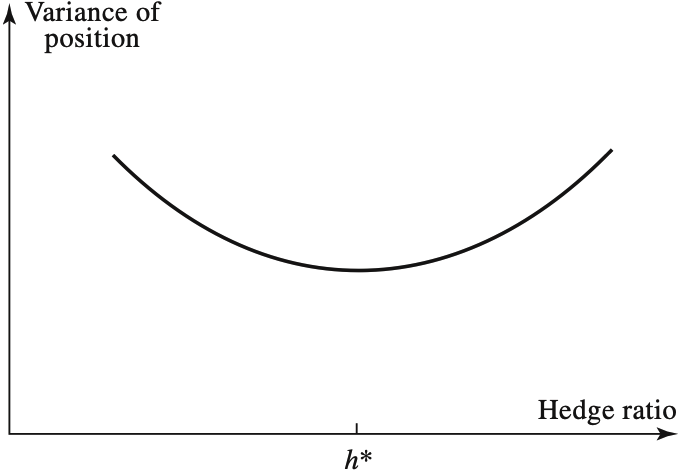
\includegraphics[scale=0.5]{derivatives/hedgeratio}
\caption{Dependence of variance of position on hedge ratio.}
\end{figure}

\hlt{Hedge effectiveness} is the proportion of variance eliminated by hedging. This is $R^2$ from regression of $\Delta S$ against $\Delta F$, and equals $\rho^2$. Parameters $\rho$, $\sigma_S$, $\sigma_F$ are estimated from historical data on $\Delta S$ and $\Delta F$.\\

The optimal number of futures to be used in hedging is
\begin{equation}
N^* = \frac{h^* Q_A}{Q_F} \nonumber
\end{equation}
where $Q_A$ is size of potion being hedged (units), $Q_F$ is size of one futures contract (units). The futures contract should be on $h^* Q_A$ units of the asset.\\

If daily settlement is used, there are a series of one-day hedges, and thus let $\hat{\sigma}_S, \hat{\sigma}_F$ be standard deviation of percentage one-day changes in spot and future price respectively, $\hat{\rho}$ be correlation between percentage one-day changes in spot and future prices. The optimal one day hedge is then
\begin{equation}
h^* = \hat{\rho}\frac{\hat{\sigma}_S S}{\hat{\sigma}_F F} \nonumber
\end{equation} 
and the optimal number of futures to be used is then
\begin{equation}
N^* = \hat{\rho}\frac{\hat{\sigma}_S S Q_A}{\hat{\sigma}_F F Q_F} \nonumber
\end{equation}

If an interest $r\%$ per annum is earned or paid over the remaining life of the hedge, then the optimal number of futures is $N^* / (1+0.01r)$; this is \hlt{tailing the hedge}.\\

Stock index futures may be used to hedge a well diversified equity portfolio. Let $V_A, V_F$ be the current value of portfolio and one futures contract respectively.\\
If portfolio mirrors the index, the optimal hedge ratio is then $1.0$, and number of futures contracts to be shorted is then $N^* = \frac{V_A}{V_F}$. If portfolio do not mirror the index, then capital asset pricing model (CAPM) should be used to determine beta ($\beta$), and the number of futures contracts to be shorted is then $N^* = \beta \frac{V_A}{V_F}$, assuming maturity of futures contract is close to the maturity of the hedge.\\

If instead, the hedger wishes to change the beta of portfolio where $\beta > \beta^*$, a short position $(\beta - \beta^*)\frac{V_A}{V_F}$ is required. If $\beta < \beta^*$, then a long position $(\beta^* - \beta)\frac{V_A}{V_F}$ is required.\\

Stock index hedging is typically used when the portfolio manager is uncertain about performance of market, but is confident that the stocks in the portfolio will outperform the market. The hedger may also be planning to hold a portfolio for a long period of time and requires short-term protection in an uncertain market situation.\\

If expiration date of hedge is later than delivery dates of all futures contracts that may be used, then the hedger may \hlt{stack and roll} by closing out one futures contract and taking the same position in a futures contract with a later delivery date.

\subsubsection{Interest Rate Futures}

The \hlt{day count} defines the way in which interest accrues, and is expressed as $X/Y$, where $X$ is the way in which number of days between two dates is calculated, $Y$ is total number of days in reference period.
\begin{equation}
\text{interest earned between two dates} = \frac{X}{Y} \times \text{interest earned in reference period} \nonumber
\end{equation}
The three common day count conventions used in United States are:
\begin{enumerate}[label=\roman*.]
\setlength{\itemsep}{0pt}
\item Actual/Actual (in period): for Treasury Bond
\item $30/360$: for corporate and municipal bonds, assumes $30$ days a month and $360$ days a year
\item Actual$/360$: for money market instruments
\end{enumerate}

Prices of money market instruments are quoted using discount rate, which is interest earned as a percentage of final face value. Let $P$ be quoted price, $Y$ be cash price, $n$ remaining life of Treasury bill in calendar days:
\begin{equation}
P = \frac{360}{n}(100 - Y) \nonumber
\end{equation}

Prices of treasury bonds are quoted in dollars and thirty-seconds of a dollar, i.e., $120$-$05$ or $120\frac{5}{32}$, which is a bond value of $\$120,156.25$. The quoted price is \hlt{clean price}, and the cash paid by purchaser is \hlt{dirty price}:
\begin{equation}
\text{cash price} = \text{quoted price} + \text{accrued interest since last coupon date} \nonumber
\end{equation} 




\newpage

    % Forex Trading Section
    \newpage
    %\section{Currency Trading}



    % Commodities Trading Section
    \newpage
    %\section{Commodities Trading}



    % Appendix Section
    \newpage
    %\section{Appendix}

For everything that cannot be classified under algorithmic trading, but is absolutely necessary for executing the concepts.

\subsection{Visual Studio Code}

Based on the book by April \cite{speight_2020}.

\begin{figure}[H]
\centering
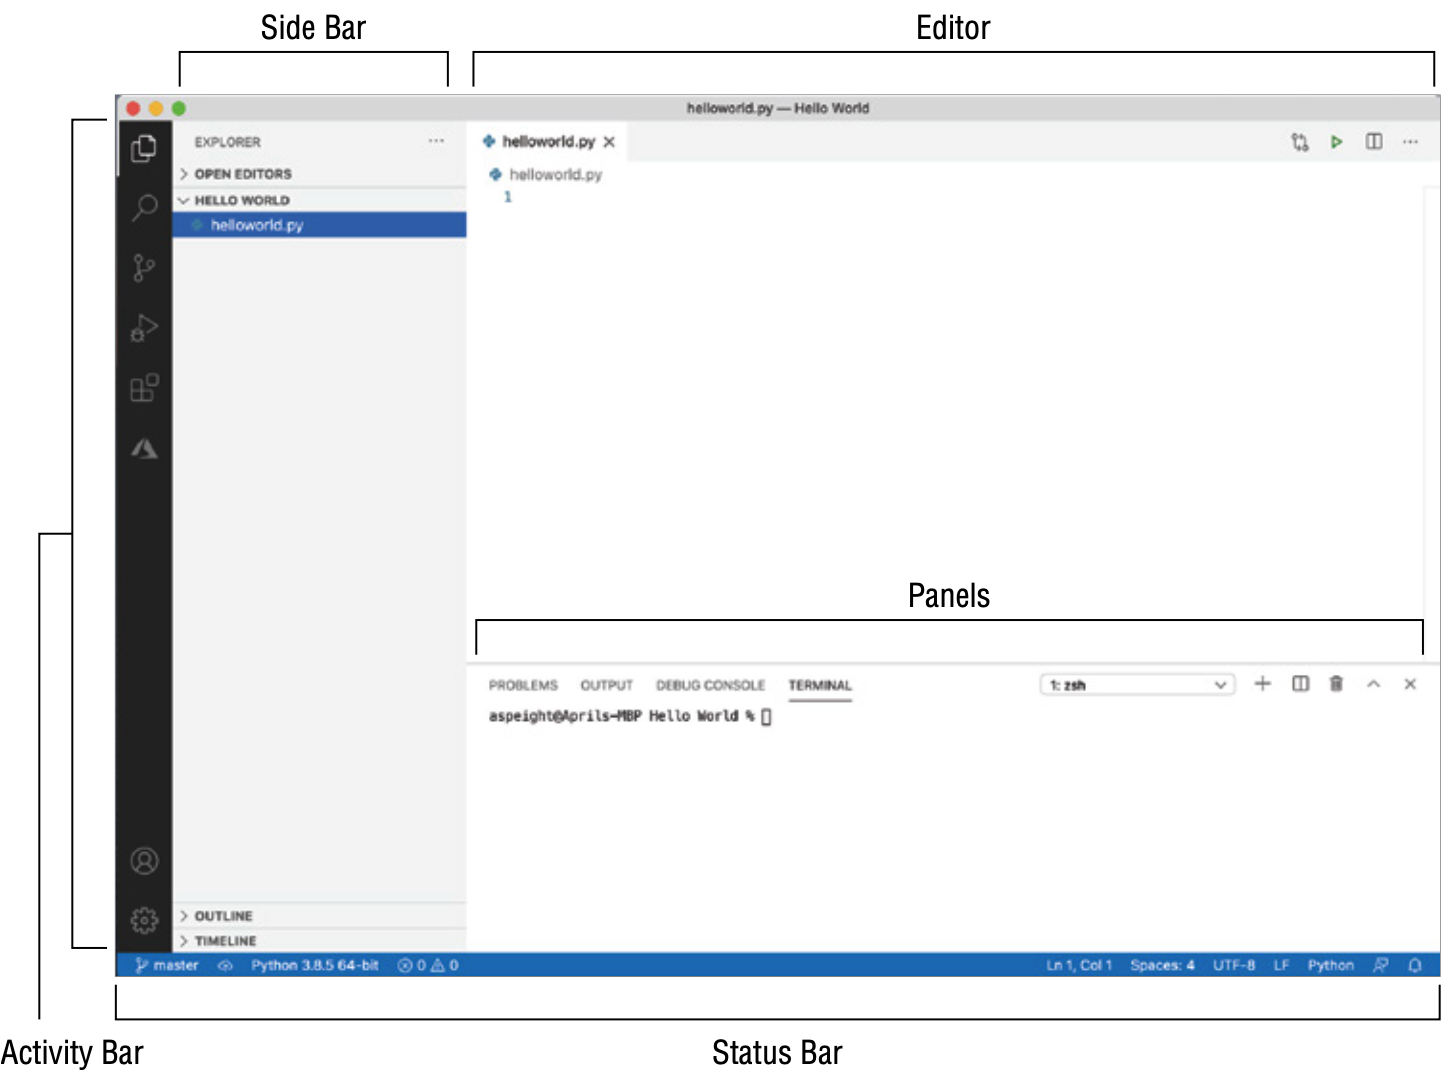
\includegraphics[scale=0.4]{appendix/vscode/vscodeui}
\caption{The visual studio code interface.}
\end{figure}

Activity bar on the far-left side allows switching between views, with quick access to tasks such as:
\begin{enumerate}[label=\roman*.]
\setlength{\itemsep}{0pt}
\item Explorer: file and folder management
\item Search: global search and replace, can use plain text or regex
\item Source Control: Git source control
\item Run: for debugging, such as variables, call stacks, breakpoints
\item Extensions: browsing, installation, management of extensions
\end{enumerate}
Activity bar may also provide custom views from extensions installed from Extension Marketplace. Views may be hidden, dragged and dropped around.\\

Side bar displays active view. Editor where files may be edited, may be resized, and top editor region changes depending on the type of file active in the editor; the top bar may also have a Source Control view if project is connected to git; files may be pinned and grouped by tabs.

\begin{figure}[H]
\centering

\includegraphics[scale=0.4]{appendix/vscode/makechanges}
\caption{Source control button}
\end{figure}

Panels are for debugging information, errors and warnings; and also for opening an integrated terminal on the root of the project. A REPL terminal (Python standard shell) may also be opened.\\

The status bar contains information about the opened project and files being edited. This includes: source control management with Git, total number of problems for the opened programs, line/column, indentation settings for space or tabs, encoding setting, end-of-line sequence setting, language mode, VS Code feedback mechanism, and notifications.\\

The command palette at the very top of the UI can be used to run commands to execute editor tasks in addition to extension commands.\\

\subsubsection{Setting Up Python}

To set default interpreter path in VS Code, in settings editor, search for \hlt{python.pythonPath}. In Python: Default Interpreter Path setting, enter the path to the interpreter.\\

To enable Quick Fix which help fix issues identified by warnings or errors (with lightbulb popping up), in settings editor, search for \hlt{python.jediEnabled}, then set it to false.\\

IntelliSense is a variety of tools to assist wth programming, such as code completion, object definition, location of object or variable declarations. These are triggered by either pressing Ctrl+Spacebar, or by tying a trigger character (i.e., a dot character in Python).\\

If linter detects any errors, these will be present in the Panels' Problem tab.\\

Refactoring is used to maintain functionality while improving the internal structure or architecture of a program. This should be a routine task that occurs before any updates or new features are added to a program. VS Code can help with refactoring via the following commands in Command Palette: Extract Variable, Extract Method, Sort Imports. Refactoring requires the \hlt{Rope} library.\\
Extract variable command allows extracting all similar occurrences of the same constant value of expression in multiple places, and replaces it with a variable. May be accessed via Python Refactor: Extract Variable.\\
Extract method command extracts all similar occurrences of selected expression or block, creates a new method, and replaces the expression with a method call. May be accessed via Python Refactor: Extract Method.\\
Sort imports method uses \hlt{isort} packages to consolidate specific imports from the same module into a single import statement, and organises 'import' statements in alphabetical order.\\

If a code pattern is repeated within a file or across multiple files, code snippets may be used, by searching in Command Palette for Snippets: Configure User Snippets. 

\subsubsection{Debugging}

After starting debug session, the Run view opens. As the debugger runs, the current state of variables is reflected in Variables panel, which organises variables into local and global scopes. In the editor, the Debug toolbar will appear with the following functionalities:
\begin{enumerate}[label=\roman*.]
\setlength{\itemsep}{0pt}
\item Continue (A): Runs all the code after the breakpoint up to the next breakpoint or end of program.
\item Step Over (B): Step line by line at the current scope. If current line is a function call, debugger runs the function entirely and then pauses at the next line after function call.
\item Step Into (C): Steps over each line within the function scope and any additional function calls.
\item Step Out (D): To exit from within a function to the scope that called it.
\item Restart (E); Stops execution and restarts the debugging session.
\item Stop (F): Stop all execution without finishing the program.
\end{enumerate}

\begin{figure}[H]
\centering

\includegraphics[scale=0.4]{appendix/vscode/debugtool}
\caption{Debug toolbar on Editor}
\end{figure}

The side bar also has a call stack section, which shows the whole chain of function calls leading up to the current point of execution. Useful if calls go through other files in the project.\\

Conditional breakpoint allows for stopping of the code during specific conditions to evaluate and debug.

\begin{figure}[H]
\centering
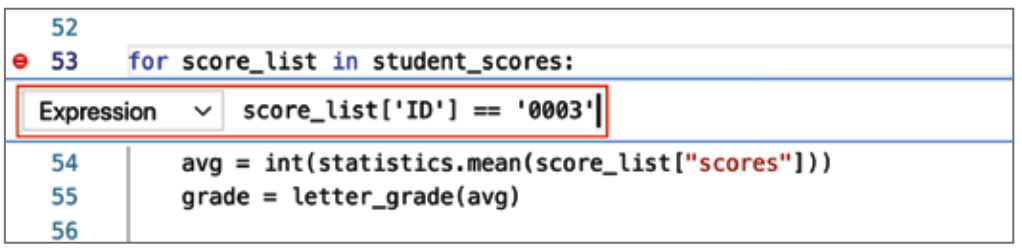
\includegraphics[scale=0.4]{appendix/vscode/condbreak}
\caption{Adding a condition in a breakpoint}
\end{figure}

A logpoint outputs message to Debug Console without breaking the debugger. Expressions can be evaluated within curly braces.

\begin{figure}[H]
\centering
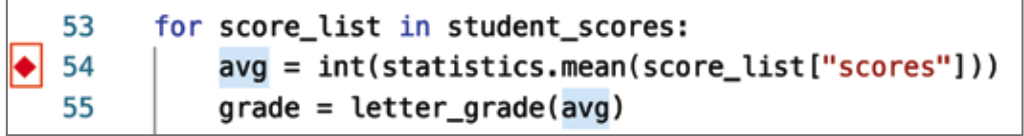
\includegraphics[scale=0.4]{appendix/vscode/logpoint}
\caption{Adding a logpoint}
\end{figure}

If program has a lot of variables which is hard to keep track of in variables pane, the variables may be added to the Watch panel which keep tracks of the variables.\\

The Debug Console allows access and modification of all the program's variables, call functions, evaluate expressions, and whatever code in the program's current state, rather than modifying the code and restarting. Different scenarios may be tested in the Debug Console and copy the fix into the program while the debugger is paused. The Debug Console also shows suggestions as code is typed.\\

To enable a test framework, \hlt{pytest} or \hlt{unittest} must be installed. Run the command Python: Configure Test to select the framework, directory that contains the test, and pattern to identify test files.
\begin{enumerate}[label=\roman*.]
\setlength{\itemsep}{0pt}
\item unittest: Looks for any Python file with 'test' in the name in top-level project folder. All test files must be importable modules or packages. To specify discovery pattern, change the pattern in \hlt{python.testing.unitTestArgs}.
\item pytest: Looks for any Python file beginning with 'test\_' or ends with '\_test' located anywhere within current folder and all subfolders.
\end{enumerate}



%\newpage

%\subsection{Python}

Covering some very useful cases of Python code for development. Based on books by Allen \cite{downey_2016}, Luciano \cite{ramalho_2016}, and...

\subsubsection{Directory and Files}

To work with files and directory, use the following snippet of code to get current path:
\begin{lstlisting}[language=Python]
import os
cwd = os.getcwd()
\end{lstlisting}
To find absolute path of file:
\begin{lstlisting}[language=Python]
filepath = os.path.abspath('file.txt')
\end{lstlisting}
To get parent folder of current file:
\begin{lstlisting}[language=Python]
parentfolder = os.path.dirname(cwd)
\end{lstlisting}
To check if file or directory exists:
\begin{lstlisting}[language=Python]
os.path.exists('file.txt')
\end{lstlisting}
To check if following is a directory, or is a file
\begin{lstlisting}[language=Python]
os.path.isdir('/dir/subdir')
os.path.isfile('file.txt')
\end{lstlisting}
To get list of files in given directory
\begin{lstlisting}[language=Python]
os.listdir(cwd)
\end{lstlisting}

For modules, the files should have the following code:
\begin{lstlisting}[language=Python]
if __name__ == '__main__':
	print(func(var1)) # Do something
\end{lstlisting}
If this code is ran as script, then '\_\_main\_\_' will run; if code is imported as module, then this is skipped.

\subsubsection{Python Data Model}

Special methods are methods that are meant to be called by the Python interpreter, and is usually implicit. To invoke a special method, call the related builtin function (e.g., len, iter, str, etc.). These are faster than method calls. The methods can be emulated in classes as follows:
\begin{enumerate}[label=\roman*.]
\setlength{\itemsep}{0pt}
\item Numeric Types: corresponding to operators such as $+$. An example in Euclidean space
\begin{lstlisting}[language=Python]
def __abs__(self):
	return math.hypot(self.x, self.y)
	
def __add__(self, value):
	return Object(self.x + value.x, self.y + value.y)

def __mul__(self, scalar):
	return Object(self.x * scalar, self.y * scalar)
\end{lstlisting}
\item String Representation: f-string gets standard representations of attributes to be displayed, which can then be used with the print function
\begin{lstlisting}[language=Python]
def __repr__(self):
	return f'Object({self.x}, {self.y})'
\end{lstlisting}
\item Boolean Type: for calling the object in a Boolean context
\begin{lstlisting}[language=Python]
def __bool__(self):
	return bool(self.x or self.y)
\end{lstlisting}
\end{enumerate}

The overview of special methods in Python is as follows:
\begin{figure}[H]
\centering
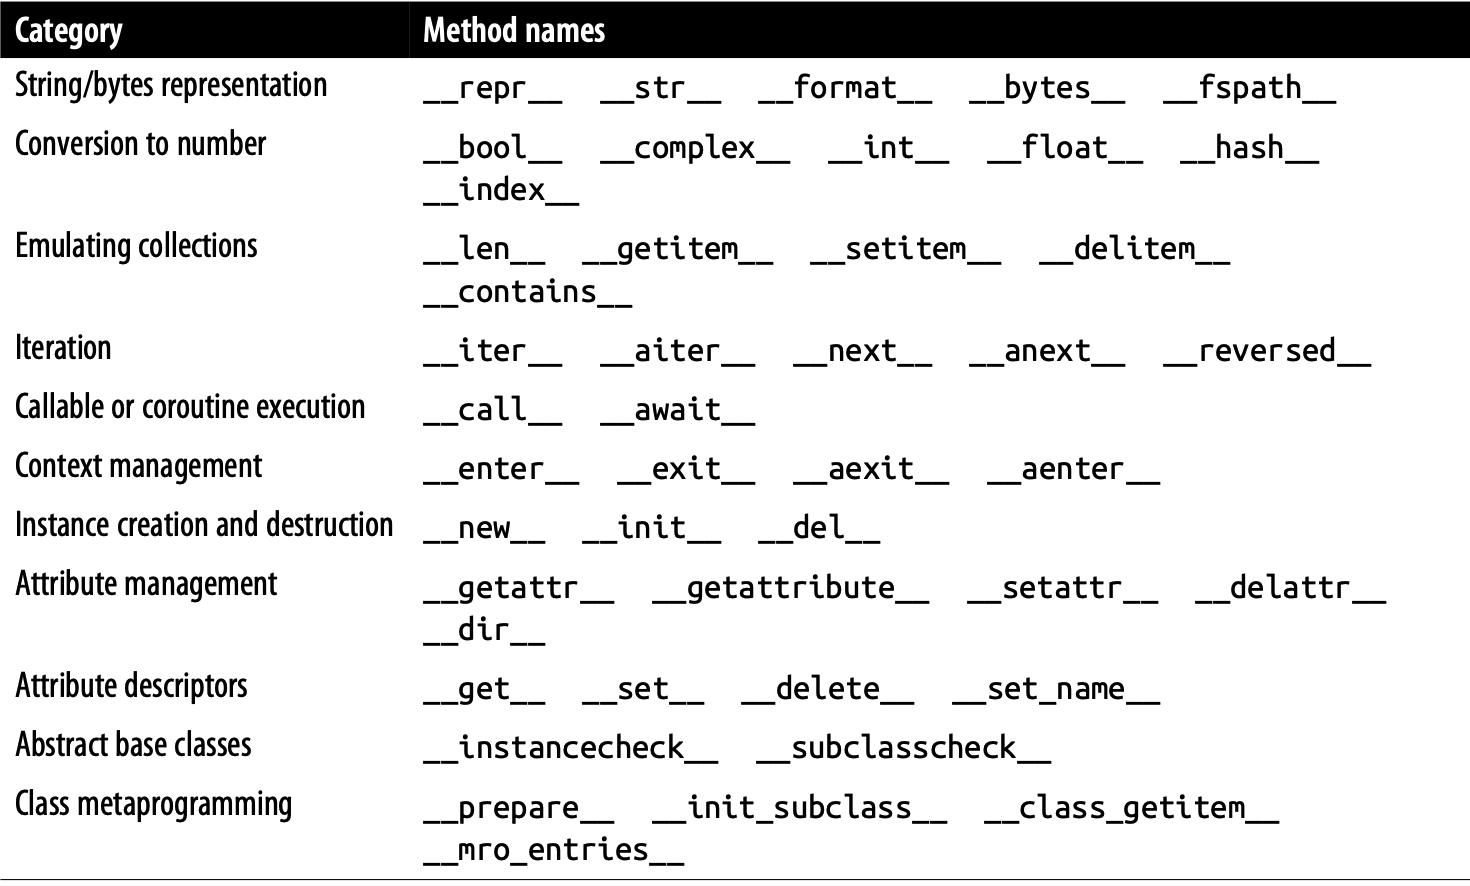
\includegraphics[scale=0.5]{appendix/python/specialmethods}
\caption{Special methods in Python}
\end{figure}


\end{comment}

\newpage
\bibliography{references}

\end{document}
	